\documentclass[a4paper,11pt]{ltjsarticle}

% ========== package ========== %
% --- 数式環境 --- %
\usepackage{amsmath}
\usepackage{amssymb}
\usepackage{mathtools}
% --- 数式環境 END --- %
% ブラケット
\usepackage{braket}
% ベクトルの太文字
\usepackage{bm}
% 添え字左右上下 \fourIdx{左上}{左下}{右上}{右下}{ベース} で使う．Iは大文字
\usepackage{fouridx}
% 色
\usepackage{color}
% 余白指定
\usepackage{geometry}
% --- ページ内リンク --- %
\usepackage{hyperref}
\hypersetup{colorlinks=true,linkcolor=blue}
% --- ページ内リンク END --- %
% 花文字
\usepackage{mathrsfs}
% 画像
\usepackage{graphicx}
% tcolorbox
\usepackage{tcolorbox}
% appendix
\usepackage{appendix}
% --- 参考文献 --- %
\usepackage{etoolbox}
\usepackage{fontspec} % fontspecは読み込んでOKですが、設定順序に注意が必要です
%% --- 参考文献フォント --- %%
  \IfFontExistsTF{Times New Roman}{
    \newfontfamily\bibfontface{Times New Roman}
  }{
    \newfontfamily\bibfontface{FreeSerif} % 代替フォント
  }
%% --- 参考文献フォント END --- %%
%% --- 参考文献リンク位置 --- %%
  \BeforeBeginEnvironment{thebibliography}{%
    \phantomsection
    \addcontentsline{toc}{section}{参考文献}
  }
  \AtBeginEnvironment{thebibliography}{%
    \normalfont\bibfontface
  }
%% --- 参考文献のリンク位置 --- %%
% --- 参考文献 END --- %
% ========== package END ========== %

% ========== newcommand ========== %
% --- セクションから目次へのリンク --- %
\newcommand{\sectionlink}[1]{\section[#1]{\hyperlink{toc}{#1}}}
\newcommand{\subsectionlink}[1]{\subsection[#1]{\hyperlink{toc}{#1}}}
% セクション番号リンク
\makeatletter
\renewcommand{\@seccntformat}[1]{%
  \protect\hyperlink{toc}{\csname the#1\endcsname}\quad
}
\makeatother

\numberwithin{equation}{section}
% ==========- newcommand END ========== %
\allowdisplaybreaks
%===========================================================
% --- タイトル --- %
%===========================================================
\geometry{left=25mm, right=25mm, top=30mm, bottom=30mm}

% ========== 原論文の数式・図表に必要な拡張 ========== %
\usepackage{amsthm,xspace,relsize,tabularx,multirow,lscape,slashed,empheq,upgreek,xfrac}
\usepackage[makeroom]{cancel}
\usepackage{floatrow}
\usepackage[labelfont=bf,labelformat=simple]{subfig}
\floatsetup[figure]{style=plain,subcapbesideposition=top}
\tcbuselibrary{most}
\usepackage{tikz-feynman}
\tikzfeynmanset{compat=1.0.0}
\newcolumntype{P}[1]{>{\centering\arraybackslash}p{#1}}
\hypersetup{unicode=true,pdftitle={インフレーションの開放有効場理論},pdfauthor={Santiago Agui Salcedo, Thomas Colas, Enrico Pajer},citecolor=blue,urlcolor=blue}
\setcounter{tocdepth}{3}
\setcounter{secnumdepth}{3}
\newcommand{\subsubsectionlink}[1]{\subsubsection[#1]{\hyperlink{toc}{#1}}}
\setlength{\emergencystretch}{3em}
\makeatletter
\g@addto@macro\bfseries{\boldmath}
\DeclareRobustCommand*\uell{{\mathpalette\@uell\relax}}
\newcommand*\@uell[2]{\setbox0=\hbox{#1\ell#1\ell}\setbox1=\hbox{\rotatebox{10}{#1\ell#1\ell}}\dimen0=\wd0\advance\dimen0 by -\wd1\divide\dimen0 by 2\mathord{\lower 0.1ex\hbox{\kern\dimen0\unhbox1\kern\dimen0}}}
\makeatother
\newcommand{\ds}{\displaystyle}
\newcommand{\ovl}[1]{\overline{#1}}

\def\piq{\pi_{\text{q}}}
\def\picl{\pi_{\text{cl}}}
\def\uppiq{\uppi_{\text{q}}}
\def\uppicl{\uppi_{\text{cl}}}

\def\pia{\pi_{a}}
\def\pir{\pi_{r}}
\def\uppia{\uppi_{a}}
\def\uppir{\uppi_{r}}

\def\bfk{\textbf{k}}
\def\bfq{\textbf{q}}

\newcommand{\enr}[1]{{\color{red} EP: #1}}
\newcommand{\TC}[1]{{\color{orange} TC: #1}}
\newcommand{\TCc}[1]{{\color{orange}#1}}
\newcommand{\SAS}[1]{{\color{blue} SAS: #1}}
\newcommand{\SASc}[1]{{\color{blue}#1}}
\renewcommand{\H}{\mathcal{H}}
\renewcommand{\O}{\mathcal{O}}
\renewcommand{\L}{\mathcal{L}}
\newcommand{\Os}{\delta \mathcal{O}_{S}}
\newcommand{\ie}{\textsl{i.e.}~}
\newcommand{\cf}{\textsl{cf.}\xspace}
\newcommand{\eg}{\textsl{e.g.}\xspace}
\newcommand{\etal}{\textsl{et al.}\xspace}
\newcommand{\apriori}{{a priori}\xspace}
\newcommand{\etc}{\textsl{etc.}\xspace}
\newcommand{\mean}[1]{\left\langle #1 \right\rangle}
\newcommand{\order}[1]{\mathcal{O}\!\left(#1\right)}
\newcommand{\Li}[1]{\mathrm{Li}_{#1}}
\DeclareMathOperator{\Ei}{Ei}
\DeclareMathOperator{\Ai}{Ai}
\DeclareMathOperator{\Bi}{Bi}
\newcommand{\Tr}{\mathrm{Tr}}

\newcommand{\cl}{\mathrm{cl}}
\newcommand{\q}{\mathrm{q}}
\newcommand{\largemathxl}[1]{{\mathlarger{#1}}}
\newcommand{\largemathxxl}[1]{{\mathlarger{\mathlarger{#1}}}}
\newcommand{\largemathxxxl}[1]{{\mathlarger{\mathlarger{\mathlarger{#1}}}}}
\newcommand{\mathlargerxxxxl}[1]{{\mathlarger{\mathlarger{\mathlarger{\mathlarger{#1}}}}}}
\newcommand{\mathlargerxxxxxl}[1]{{\mathlarger{\mathlarger{\mathlarger{\mathlarger{\mathlarger{#1}}}}}}}
\newcommand{\mathlargerxxxxxxl}[1]{{\mathlarger{\mathlarger{\mathlarger{\mathlarger{\mathlarger{\mathlarger{#1}}}}}}}}
\newcommand{\mathlargerxxxxxxxl}[1]{{\mathlarger{\mathlarger{\mathlarger{\mathlarger{\mathlarger{\mathlarger{\mathlarger{#1}}}}}}}}}
\newcommand{\mathlargerxxxxxxxxl}[1]{{\mathlarger{\mathlarger{\mathlarger{\mathlarger{\mathlarger{\mathlarger{\mathlarger{\mathlarger{#1}}}}}}}}}}
\newcommand{\mathlargerxxxxxxxxxl}[1]{{\mathlarger{\mathlarger{\mathlarger{\mathlarger{\mathlarger{\mathlarger{\mathlarger{\mathlarger{\mathlarger{#1}}}}}}}}}}}
\newcommand{\mathlargerxxxxxxxxxxl}[1]{{\mathlarger{\mathlarger{\mathlarger{\mathlarger{\mathlarger{\mathlarger{\mathlarger{\mathlarger{\mathlarger{\mathlarger{#1}}}}}}}}}}}}
\newcommand{\lta}{\lesssim}
\newcommand{\gta}{\gtrsim}
\newcommand{\dd}{\mathrm{d}}
\newcommand{\ee}{e}
\newcommand{\sss}[1]{{\scriptscriptstyle{#1}}}
\newcommand{\boldmathsymbol}[1]{{\ensuremath{\boldsymbol{#1}}}}

\newcommand{\uPl}{\mathrm{Pl}}
\newcommand{\uin}{\mathrm{in}}
\newcommand{\umin}{\mathrm{min}}
\newcommand{\umax}{\mathrm{max}}
\newcommand{\uend}{\mathrm{end}}
\newcommand{\uini}{\mathrm{ini}}
\newcommand{\ueff}{\mathrm{eff}}
\newcommand{\uinf}{\mathrm{inf}}
\newcommand{\ureh}{\mathrm{reh}}
\newcommand{\urad}{\mathrm{rad}}
\newcommand{\utop}{\mathrm{top}}
\newcommand{\ucri}{\mathrm{cri}}
\newcommand{\ucl}{\mathrm{cl}}
\newcommand{\unuc}{\mathrm{nuc}}
\newcommand{\uobs}{\mathrm{obs}}
\newcommand{\ulim}{\mathrm{lim}}
\newcommand{\uphys}{\mathrm{phys}}
\newcommand{\uPgiP}{\mathrm{(gi)}}
\newcommand{\ue}{\mathrm{e}}
\newcommand{\uc}{\mathrm{c}}
\newcommand{\ub}{\mathrm{b}}
\newcommand{\us}{\mathrm{s}}
\newcommand{\uS}{\mathrm{S}}
\newcommand{\uM}{\mathrm{M}}
\newcommand{\uPSP}{(\uS)}
\newcommand{\uV}{\mathrm{V}}
\newcommand{\uT}{\mathrm{T}}
\newcommand{\uPTP}{(\uT)}
\newcommand{\uE}{\mathrm{E}}
\newcommand{\usssTE}{\sss{\uT \uE}}
\newcommand{\usssS}{\sss{\uS}}
\newcommand{\usssPSP}{\sss{\uPSP}}
\newcommand{\usssT}{\sss{\uT}}
\newcommand{\usssPTP}{\sss{\uPTP}}
\newcommand{\usssPMoneP}{\sss{(\uM=1)}}
\newcommand{\usssPl}{\sss{\uPl}}
\newcommand{\usssRH}{\ureh}
\newcommand{\usssV}{\sss{\uV}}
\newcommand{\usssE}{\sss{\uE}}
\newcommand{\nS}{n_\usssS}
\newcommand{\nT}{n_\usssT}
\newcommand{\alphaS}{\alpha_\usssS}
\newcommand{\alphaT}{\alpha_\usssT}
\newcommand{\zero}{{_0}}
\newcommand{\one}{{_1}}
\newcommand{\two}{{_2}}
\newcommand{\udm}{\mathrm{dm}}
\newcommand{\ud}{\mathrm{d}}
\newcommand{\muS}{\mu_\usssS}
\newcommand{\muT}{\mu_\usssT}
\newcommand{\muST}{\mu_{\usssS,\usssT}}
\newcommand{\uRL}{\mathrm{RL}}
\newcommand{\uNL}{\mathrm{NL}}
\newcommand{\uwkb}{\mathrm{WKB}}

\newcommand{\bmk}{\boldmathsymbol{k}}
\newcommand{\bmx}{\boldmathsymbol{x}}

\newcommand{\calH}{\mathcal{H}}
\newcommand{\calP}{\mathcal{P}}
\newcommand{\calG}{\mathcal{G}}
\newcommand{\calO}{\mathcal{O}}
\newcommand{\calI}{\mathcal{I}}

\newcommand{\setR}{\mathbb{R}}
\newcommand{\setC}{\mathbb{C}}

\newcommand{\Rea}{\Re \mathrm{e}\,}
\newcommand{\Ima}{\Im \mathrm{m}\,}

\newcommand{\Real}[1]{\Rea \left[ #1 \right] }
\newcommand{\Imag}[1]{\Ima \left[ #1 \right] }
\newcommand{\eV}{\mathrm{eV}}
\newcommand{\keV}{\mathrm{keV}}
\newcommand{\MeV}{\mathrm{MeV}}
\newcommand{\GeV}{\mathrm{GeV}}
\newcommand{\TeV}{\mathrm{TeV}}
\newcommand{\cm}{\mathrm{cm}}
\newcommand{\km}{\mathrm{km}}
\renewcommand{\sec}{\mathrm{s}}
\newcommand{\pc}{\mathrm{pc}}
\newcommand{\kpc}{\mathrm{kpc}}
\newcommand{\Mpc}{\mathrm{Mpc}}
\newcommand{\K}{\mathrm{K}}

\newcommand{\Hu}{\mathcal{H}}
\newcommand{\Ka}{\mathcal{K}}
\newcommand{\Zed}{\mathcal{Z}}
\newcommand{\cs}{c_{_\mathrm{S}}}
\newcommand{\omegaT}{\omega_\usssT}
\newcommand{\omegaS}{\omega_\usssS}
\newcommand{\omegaST}{\omega_{\usssS, \usssT}}
\newcommand{\OmegaL}{\Omega_\Lambda}
\newcommand{\OmegaCDM}{\Omega_\udm}
\newcommand{\OmegaB}{\Omega_\ub}
\newcommand{\OmegaR}{\Omega_\gamma}
\newcommand{\Qrms}{Q_{\mathrm{rms-PS}}}
\newcommand{\wstate}{w}
\newcommand{\Mc}{M_\uc}
\newcommand{\potS}{U_{_\uS}}
\newcommand{\potT}{U_{_\uT}}

\newcommand{\mpl}{m_\usssPl}
\newcommand{\Mp}{M_\usssPl}
\newcommand{\Hzero}{H_0}
\newcommand{\Hstar}{H_*}
\newcommand{\kstar}{k_*}
\newcommand{\Pstar}{P_*}
\newcommand{\astar}{a_*}
\newcommand{\Pnum}{P^{\usssPMoneP}}
\newcommand{\calNnuc}{\mathcal{N}^\unuc}
\newcommand{\calNend}{\mathcal{N}^\uend}
\newcommand{\calFnuc}{\mathcal{F}^\unuc}
\newcommand{\calFend}{\mathcal{F}^\uend}
\newcommand{\rRL}{r_\uRL}
\newcommand{\fnl}{f_\uNL}
\newcommand{\csini}{c_{\us \uini}}

\newcommand{\etastar}{\eta_*}
\newcommand{\nustar}{\nu_*}
\newcommand{\csstar}{c_{\us*}}
\newcommand{\epsonestar}{\epsilon_{1*}}
\newcommand{\epstwostar}{\epsilon_{2*}}
\newcommand{\epsthreestar}{\epsilon_{3*}}
\newcommand{\deltaonestar}{\delta_{1*}}
\newcommand{\deltatwostar}{\delta_{2*}}
\newcommand{\epsnstar}{\epsilon_{n*}}
\newcommand{\epsnponestar}{\epsilon_{n+1*}}
\newcommand{\xstar}{x_*}

\newcommand{\ustar}{u_*}
\newcommand{\wstar}{w_*}

\newcommand{\dia}{\sss{\diamond}}
\newcommand{\Hdia}{H_\dia}
\newcommand{\kdia}{k_\dia}
\newcommand{\etadia}{\eta_\dia}
\newcommand{\csdia}{c_{\us \dia}}
\newcommand{\epsonedia}{\epsilon_{1\dia}}
\newcommand{\epstwodia}{\epsilon_{2\dia}}
\newcommand{\epsthreedia}{\epsilon_{3\dia}}
\newcommand{\epsfourdia}{\epsilon_{4\dia}}
\newcommand{\epsfivedia}{\epsilon_{5\dia}}

\newcommand{\deltaonedia}{\delta_{1\dia}}
\newcommand{\deltatwodia}{\delta_{2\dia}}
\newcommand{\deltathreedia}{\delta_{3\dia}}
\newcommand{\deltafourdia}{\delta_{4\dia}}

\newcommand{\grav}{\star}
\newcommand{\Hgrav}{H_\grav}
\newcommand{\kgrav}{k_\grav}
\newcommand{\etagrav}{\eta_\grav}
\newcommand{\epsonegrav}{\epsilon_{1\grav}}
\newcommand{\epstwograv}{\epsilon_{2\grav}}

\newcommand{\aH}{\sss{\circledast}}
\newcommand{\kah}{k_\aH}
\newcommand{\etaah}{\eta_\aH}

\newcommand{\Dwkb}{D_{_\uwkb}}
\newcommand{\Awkb}{A_{_\uwkb}}
\newcommand{\efolds}{$e$-folds~}
\newcommand{\efold}{$e$-fold}
\newcommand{\Nini}{N_\uini}
\newcommand{\Nend}{N_\uend}
\newcommand{\Nreh}{N_\ureh}
\newcommand{\Nstar}{N_*}
\newcommand{\Nzero}{N_\zero}
\newcommand{\Nstarnuc}{N_*^\unuc}
\newcommand{\Nstarend}{N_*^\uend}
\newcommand{\beq}{\begin{equation}}
	\newcommand{\eeq}{\end{equation}}
\newcommand{\bea}{\begin{equation}\begin{aligned}}
		\newcommand{\eea}{\end{aligned}\end{equation}}
\newlength{\wsingfig}
\setlength{\wsingfig}{0.99\textwidth}
\newlength{\wdblefig}
\setlength{\wdblefig}{0.49\textwidth}
\newlength{\wquadfig}
\setlength{\wquadfig}{0.249\textwidth}
\newlength{\wtriplefig}
\setlength{\wtriplefig}{0.333\textwidth}
\newcommand{\Eq}[1]{Eq.~(\ref{#1})}
\newcommand{\Eqs}[1]{Eqs.~(\ref{#1})}
\newcommand{\Fig}[1]{Fig.~{\ref{#1}}}
\newcommand{\Figs}[1]{Figs.~{\ref{#1}}}
\newcommand{\Refa}[1]{Ref.~{\cite{#1}}}
\newcommand{\Refs}[1]{Refs.~{\cite{#1}}}
\newcommand{\Sec}[1]{Sec.~\ref{#1}}
\newcommand{\Secs}[1]{Secs.~\ref{#1}}
\newcommand{\App}[1]{Appendix~\ref{#1}}
\newcommand{\Apps}[1]{Appendices~\ref{#1}}

\newcommand{\bs}[1]{\boldsymbol{#1}}



\newcommand{\cF}{ {\cal F} }
\newcommand{\cS}{ {\cal S} }
\newcommand{\cM}{ {\cal M} }
\newcommand{\bk}{ {\mathbf{k}} }
\newcommand{\bp}{ {\mathbf{p}} }
\newcommand{\by}{ {\mathbf{y}} }

\newcommand{\bN}{ {\mathbb{N}} }
\newcommand{\bC}{ {\mathbb{C}} }
\newcommand{\bQ}{ {\mathbb{Q}} }
\newcommand{\bR}{ {\mathbb{R}} }
\newcommand{\bZ}{ {\mathbb{Z}} }
\renewcommand{\qedsymbol}{$\blacksquare$}
\newcommand{\mM}{ {\mathcal{M}} }


\newcommand{\sy}{\mathsf{y}}
\usepackage{dsfont}
\newcommand{\openone}{\mathds{1}}




\newenvironment{brsm}{% % short for 'bracketed small matrix'
  \bigl[ \begin{smallmatrix} }{%
  \end{smallmatrix} \bigr]}

\newcommand{\tX}{ {\tilde{X}} }
\newcommand{\tY}{ {\tilde{Y}} }

\newcommand{\CM}{ {\mathcal{C}_{\mathrm{M}}} }
\newcommand{\WM}{ {\mathcal{W}_{\mathrm{M}}} }

\newcommand{\Ti}{ {T_{\mathrm{i}}} }
\newcommand{\Tf}{ {T_{\mathrm{f}}} }

\newcommand{\ti}{ {t_{\mathrm{i}}} }
\newcommand{\tf}{ {t_{\mathrm{f}}} }

\newcommand{\Hint}{ {H_{\mathrm{int}}} }

\def\ssI{{\scriptscriptstyle I}}
\def\ssT{{\scriptscriptstyle T}}
\def\ssD{{\scriptscriptstyle D}}

\newcommand{\bx}{ {\mathbf{x}} }
\newcommand{\bpp}{ {\mathbf{p}} }
\newcommand{\bkk}{ {\mathbf{k}} }


\newcommand{\gA}{ {g_{\mathrm{A}}} }
\newcommand{\gAsq}{ {g_{\mathrm{A}}^2} }
\newcommand{\gB}{ {g_{\mathrm{B}}} }
\newcommand{\gBsq}{ {g_{\mathrm{B}}^2} }

\newcommand{\WO}{ {\mathcal{W}_{\Omega}} }
\newcommand{\Cs}{ {\mathcal{C}_{\mathrm{self}}} }
\newcommand{\Cc}{ {\mathcal{C}_{\mathrm{cross}}} }
\newcommand{\Ss}{ {\mathcal{S}_{\mathrm{self}}} }
\newcommand{\Sc}{ {\mathcal{S}_{\mathrm{cross}}} }
\newcommand{\Ds}{ {\Delta_{\mathrm{self}}} }
\newcommand{\Dc}{ {\Delta_{\mathrm{cross}}} }
\newcommand{\Xs}{ {\Xi_{\mathrm{self}}} }
\newcommand{\Xc}{ {\Xi_{\mathrm{cross}}} }

\newcommand{\exd}{{\hbox{d}}}
\newcommand{\tT}{{\xi_{\ssT}}}
\newcommand{\tD}{{\xi_{\ssD}}}
\def\smath#1{\text{\scalebox{.85}{$#1$}}}
\def\sfrac#1#2{\smath{\frac{#1}{#2}}}
\newcommand{\vac}{{\ket{\Omega}\bra{\Omega}}}

\newcommand{\RW}{ {\mathrm{Re}[\mathcal{W}(s) ]} }
\newcommand{\IW}{ {\mathrm{Im}[\mathcal{W}(s) ]} }

\newcommand{\wA}{ {\omega_{\mathrm{A}}} }
\newcommand{\wB}{ {\omega_{\mathrm{B}}} }

\def\ssI{{\scriptscriptstyle I}}
\def\ssS{{\scriptscriptstyle S}}
\def\ssA{{\scriptscriptstyle A}}
\def\ssB{{\scriptscriptstyle B}}
\def\ssF{{\scriptscriptstyle F}}


\def\bmx{{\boldsymbol{x}}}
\def\bmy{{\boldsymbol{y}}}
\def\bmk{{\boldsymbol{k}}}
\def\bmp{{\boldsymbol{p}}}
\def\bmq{{\boldsymbol{q}}}

\def\whv{{\widehat{v}}}
\def\whp{{\widehat{p}}}
\def\wtv{{\widetilde{v}}}
\def\wtp{{\widetilde{p}}}


\def\rX{{\mathrm{X}}}




\newcommand{\vacdS}{ { 0_{\mathrm{dS} }} }


\newcommand*{\Scale}[2][4]{\scalebox{#1}{$#2$}}
\renewcommand{\Eq}[1]{式~\eqref{#1}}
\renewcommand{\Eqs}[1]{式~\eqref{#1}}
\renewcommand{\Fig}[1]{図~\ref{#1}}
\renewcommand{\Figs}[1]{図~\ref{#1}}
\renewcommand{\Sec}[1]{第~\ref{#1}~節}
\renewcommand{\Secs}[1]{第~\ref{#1}~節}
\renewcommand{\App}[1]{付録~\ref{#1}}
\renewcommand{\Apps}[1]{付録~\ref{#1}}
\title{\bfseries インフレーションの開放有効場理論}
\author{Santiago Ag\"u\'i Salcedo \and Thomas Colas \and Enrico Pajer}
\date{\href{https://arxiv.org/abs/2404.15416v2}{arXiv:2404.15416v2 [hep-th]}\\2024年11月13日}
\begin{document}
\maketitle
\begin{center}\small
Department of Applied Mathematics and Theoretical Physics, University of Cambridge,\\
Wilberforce Road, Cambridge, CB3 0WA, UK\\
\href{mailto:sa2013@cam.ac.uk}{sa2013@cam.ac.uk},
\href{mailto:tc683@cam.ac.uk}{tc683@cam.ac.uk},
\href{mailto:enrico.pajer@gmail.com}{enrico.pajer@gmail.com}
\end{center}
\begin{abstract}
宇宙論的摂動がどのように生成されたかを理解しようとすると、二つの重大な障害に直面する。第一に、インフレーション中に原始摂動が置かれていた環境について、直接の情報がない。第二に、実際に観測できる量はほぼ質量のない場の相関関数に限られ、より重い場や微分に関わる量は e-folding 数とともに指数関数的に減衰する。開放系の柔軟で一般的な枠組みは、まさにこの種の問題に対処するために発展してきた。本論文では先行研究を踏まえ、時空の局所性を鍵となる仮定として、未知の環境と相互作用する時間並進のゴールドストーン・ボソンが、散逸的かつ非ユニタリに進化しうることを記述する、インフレーションの開放有効場理論を Schwinger--Keldysh 経路積分で構成する。非結合極限で de Sitter 時空における線形理論と相互作用理論を調べ、微分展開に従って整理された有限個の有効結合に依存するパワースペクトルとバイスペクトルの予言を導く。環境との相互作用を示す決定的な特徴は、folded な運動学的極限の近傍で、増大しながらも有限にとどまるバイスペクトルである。さらに、明示的なモデルと開放有効理論を対応付け、この手法の一般性を示す。本構成は、現象論的な予言とインフレーションの量子情報的側面を同時に研究するための標準的なモデルを与える。
\end{abstract}
\hypertarget{toc}{}
\tableofcontents
\clearpage
\sectionlink{序論}

宇宙論モデルの基礎となるのは、非常に大きなスケールでの宇宙論的観測量が、熱いビッグバンの開始時における摂動の相関関数と近似的に線形な関係にある、という事実である。したがって、宇宙論的摂動の初期条件は、宇宙が再加熱されて標準模型粒子の熱浴になる以前の、未知のダイナミクスによって定まったはずである。その有力な説明であるインフレーションでは、長く続く加速膨張と、真空揺らぎの量子的生成が組み合わされる。この原始宇宙の枠組みには、いくつか特有の事情がある。まず、時間発展を直接調べることは実際にはできず、インフレーション終了時の最終結果しか見えない。後期の観測量に限っても、実際に測定できる量には厳しい制約がある。直接アクセスできるのは、系の典型的なスケール、すなわちインフレーションの Hubble スケールと比べて、質量がゼロか非常に軽い場に関する観測量だけである。軽い場は一般的なものではなく、その存在は通常、理論の何らかの対称性に由来する。典型例は重力子 \cite{Starobinsky:1979ty} で、その質量がゼロであることは一般共変性に結び付いている。原始摂動には、少なくとも数パーセントの精度でスカラー成分があると測定されている \cite{BICEPKeck:2022mhb}。したがって、インフレーション中には、これに加えて質量のないスカラーが活動していたはずである。それは曲率摂動、あるいは自発的に破れた時間並進のゴールドストーン・ボソン \cite{Cheung:2007st} と解釈できる。その近似的な無質量性は、内部シフト対称性と、ほぼ線形な背景の時間発展との重要な組合せに由来する \cite{Finelli:2018upr}。より重い場は時間とともに減衰せざるをえず、その存在は軽い場への影響などを通じて間接的にしか確かめられない。軽い場の微分についても同様で、インフレーションの e-folding 数に対して指数関数的に減衰する。このため、軽い場であっても、その共役運動量を含む相関関数を実際に調べることはできない。

系全体のうち、軽い場の相関関数の後期極限という限られた部分しか調べられないことは、インフレーションをモデル化する理論的枠組みに重要な意味をもつ。後期に減衰する場も含めて系全体をモデル化し、閉鎖系に適した枠組みを用いることはできる。一方、観測する部分系、すなわち質量のない曲率摂動に焦点を当て、\textit{開放系}の枠組みで扱うほうが有利かもしれない。開放系と閉鎖系の違いは、さまざまな形で現れる。第一に、閉鎖系では保存量を正確に追跡し、その制約を利用できるが、開放系の観測可能なダイナミクスには、その制約が大幅に緩む。第二に、開放系では、以後「\textit{環境}」と呼ぶ系の残りの部分との相関を追跡する必要がある。この点は統計理論や確率理論などの古典的な時間発展にも当てはまるが、量子系では特に重要である。閉鎖系ではあらゆる履歴を考慮するのに対し、開放系では情報が環境へ失われうるため、確率を予言する仕方が大きく異なる。

本研究は、必然的に有効モデルに依存するインフレーション中の量子ダイナミクスを十分かつ包括的に理解するには、一般的で柔軟な\textit{開放量子系}の枠組みから始めなければならない、という認識に基づく。これは理論面と観測面の双方で必要な出発点と考えられる。観測面では、本論文の以下で論じるように、曲率摂動への大きな環境効果が、データから探索すべき新しい信号を生む。理論面では、真空から摂動が生成され、エネルギーが保存せず、長さと時間のスケールが動的な概念となり、情報が大域的に再分配される加速時空に、平坦時空の有効場理論（EFT）の規則と Wilson 的パラダイムをどのように移すかを理解する必要がある。

具体的な設定をいくつか挙げよう。まず、単一のスカラー場が緩やかにスローロールする、もっとも単純なインフレーション模型を考える。この場合でさえ、Hubble 膨張のため、観測する曲率摂動は平坦時空と同じ真空を経験しない。代わりに、de Sitter 温度 $H/2\pi$ にある場の励起の、ほぼ熱的な浴と相互作用する。この浴には理論のあらゆる自由度が含まれ、重い自由度も例外ではない。提案する EFT の有効範囲を把握し、予言への補正を正しく見積もるには、環境との相互作用を評価し、いつ無視できるかを判断したい。もっとも単純な場合、重い場の励起は Boltzmann 因子によって抑制されると予想される（例えば \cite{Arkani-Hamed:2015bza,Tong:2021wai} を参照）。しかし、この抑制を打ち消す仕組みとして、de Sitter の boost 不変性の大きな破れ \cite{Lee:2016vti}、化学ポテンシャル \cite{Chen:2018xck,Wang:2019gbi,Bodas:2020yho,Tong:2022cdz,Sou:2021juh}、タキオン的質量 \cite{McCulloch:2024hiz} など、さまざまな可能性が考えられてきた。より一般には、多くの模型に熱的な de Sitter 放射を超える粒子生成機構がある。古くからある温かいインフレーション \cite{Berera:1995wh,Berera:1995ie,Berera:2023liv} では、Hubble 膨張に抗する連続的な供給源によって放射浴が維持される。多くの設定では環境が非熱的に満たされる。よく研究されている例は、ゆっくり転がる場 $\phi$ と $\phi F\tilde F$ の結合によって生じる、一方の helicity のゲージ場のタキオン的生成である \cite{Anber:2009ua}。この場合、宇宙は Hubble 程度の波長のゲージ場励起で満たされる。励起は膨張で希釈・赤方偏移する一方、連続的に生成される。このほかにも多くの可能性が考えられてきたが、ここでは網羅的には列挙しない。要点は、最小の設定でも非最小の設定でも、遍在する環境との相互作用を許す曲率揺らぎのダイナミクスの記述が望ましい、ということである。その記述があれば、その相互作用が重要となる領域と、安全に無視できる領域を、より正確に特定できる。

インフレーション中にありうる環境は無数で、その性質は模型に全面的に依存する。それでも、統一的な記述と少数の特徴的予言に到達できるだろうか。そのためには開放量子系の EFT を用いるのが自然である。まず、EFT に万能の力はない。一般の設定では、両者が強く結合していたり、利用可能な荷によって明確に分離できなかったりして、関心のある系と環境を区別できるとは限らない。EFT が整理原理として役立つのは、対称性などによって明確な分離が与えられ、スケールの階層が存在するときである。そこで本論文では、Hubble 半径通過の付近で、未知の環境を曲率摂動のセクターから分離できる場合を考える。環境の摂動は、より速い時間発展、すなわち高い周波数と、より短い距離、すなわち高い運動量を特徴とする。この領域では、環境を含めた系全体を詳細に記述する場合と異なり、環境の少数の性質を指定するだけで曲率摂動の進化を正確に記述できると期待される。その少数の性質は、系の\textit{開放 EFT} における Wilson 的な有効結合によって指定される。

EFT の本質的な特徴は、有限の精度を目標とする限り、考慮すべき相互作用が有限個で済むことである。この有限性はしばしば\footnote{ほかの可能性もある。一部の非局所 EFT では、Fermi 面の励起や特定の非局所性の部分的な再総和のように、異なる整理原理が存在しうる。}、EFT のダイナミクスが時空で局所的であるという仮定によって保証される。本論文はこの仮定を置き、議論と結果はこの重要な性質に依存する。環境が Hubble スケール付近で相互作用を媒介する模型は、ここでの記述の範囲外である。これは開放系に固有の問題ではない。標準的な EFT でも、対象のスケールで活動する自由度を積分消去すると、扱いにくい非局所相互作用が生じ、高エネルギー側の具体的な理論を知らなければ EFT は力を発揮しない。こうした状況には有用なスケール階層がなく、EFT による自然な整理が存在しないのである。

閉鎖系として記述されるインフレーションについては、インフレーションの有効場理論（EFToI）\cite{Cheung:2007st} が強力な整理原理となっている。この考え方を開放系へ一般化する先駆的研究が二つあり、本研究はそれらを踏まえる。第一の研究 \cite{LopezNacir:2011kk} は、時間並進のゴールドストーン・ボソン $\pi$ が環境のノイズ揺らぎと結合し、さらに散逸的に進化しうる状況を調べた。その中心となる道具は、古典的な運動方程式を確率的に一般化した \textit{Langevin 方程式}である。これによって非常に一般的な開放系のダイナミクスをモデル化し、特徴的な信号を特定できる。この手法では、Lagrangian や Hamiltonian に関わる汎関数的手法を脇に置き、運動方程式を直接扱う。これは系統的な記述を与える一方、いくつかの弱点もある。第一に、対称性とそれに対応する荷や流れは、作用や Lagrangian の文脈で自然に論じられる。第二に、一見すると、Schwinger--Keldysh（in-in）形式の演算子または経路積分によって閉鎖系のインフレーションを調べる通常の方法と、本質的に異なるように見える。しかし Schwinger--Keldysh 形式は、そもそも開放系を研究するために発展した。散逸や揺らぎ、関連する現象を扱うのに、これを捨てる必要はない。

近年の研究 \cite{Crossley:2015evo,Glorioso:2017fpd,Liu:2018kfw} によって、高エネルギー分野、とりわけ流体力学における Schwinger--Keldysh 形式への関心が再び高まっている。これらの研究は、想定した開放有効理論が、系全体に対して整合的、すなわちユニタリで局所的かつ因果的な理論から環境を積分消去して実際に得られるための、一般的な規則の一部を明らかにした。流体力学と同様に、インフレーションでも自発的対称性の破れを用いて系を同定することに関心がある。一般に流体力学的モードは、保存荷を伴う可能性のある、大域的な熱平衡からの小さな局所的ずれのダイナミクスを記述すると考えられる。宇宙論で関心のある系は、それと同様に、インフラトン・セクターの時間発展によって自発的に破れた時間並進のゴールドストーン・ボソンである。この時間発展は時空に好ましい葉層構造を選ぶ。この文脈でのゴールドストーン・ボソンの開放 EFT の研究は \cite{Hongo:2018ant} に始まる（関連研究 \cite{Hongo:2019qhi} も参照）。そこで、平坦時空における $\pi$ の二次理論が導かれ、研究された。本研究はその探究を宇宙論的時空へ進め、相互作用と非ガウス性の生成を含める。時間のない読者のため、主な結果を \Sec{summary} にまとめる。

本手法を先行研究と比較しておこう。まず、宇宙論的相関関数に対して最近提案された \textit{in-out 形式} \cite{Donath:2024utn} を考える。この研究では、閉鎖系がユニタリな Hamiltonian 発展に従うなら、de Sitter 時空の宇宙論的相関関数を、平坦時空の散乱振幅と同じ in-out 形式、すなわち単一の時間順序 Feynman 伝播関数だけを使う Feynman 則によって計算できることが指摘された。一方、より煩雑な in-in 形式では、四種類のバルク間伝播関数と二種類のバルク・境界間伝播関数が現れ、図の $V$ 個の頂点それぞれを、左側の時間発展または右側の反時間発展のどちらに属させるかという $2^V$ 通りの指定に応じて組み合わされる。赤外で有限な相互作用に対して in-out 形式は大幅な簡略化を与え、\cite{Arkani-Hamed:2017fdk} の波動関数の再帰関係に対応する相関関数の関係、Cutkosky と Veltman の規則に完全に類似した相関関数の切断則、de Sitter の S 行列の自然な定義などを導きやすくする。しかし、開放系が存在すると in-in と in-out の等価性は成り立たない。したがってこの方法が適用されるのは、本研究で扱う理論を除いた領域である。

開放量子系の手法は、これとはまったく別の目的でもインフレーションに用いられてきた。すなわち、特定の永年的な発散を再総和し、時間の対数項があるときの摂動論の妥当性を回復するためである \cite{Burgess:2015ajz,Burgess:2024eng}。これは確率的インフレーション \cite{Starobinsky:1986fx,Starobinsky:1994bd} と、de Sitter 時空で生じる赤外の問題 \cite{Gorbenko:2019rza,Cespedes:2023aal} の研究に広く使われている。強調したいのは、本研究で開放系を扱う動機はそれとは独立しているという点である。ここで調べる模型はすべて赤外で有限であり、赤外の再総和を必要としない。曲がった時空が、互いに同等でない複数の仕方で開放系の記述を促すのは興味深い。宇宙論で開放系の手法を用いたほかの研究にも、必要に応じて言及する。

\paragraph{用語法} 開放・非平衡量子ダイナミクスを記述する用語は、分野によってさまざまである。\footnote{この問題についての議論に関して C. Burgess に感謝する。} 高エネルギー・素粒子物理では、しばしば状態の規格化の保存、すなわち次式によりユニタリ性を定義する。

\begin{align}
\frac{\dd }{\dd t} \mathrm{Tr}[\rho]  = 0,
\end{align}

ここで $\rho$ は系の密度行列である。一方、量子光学や凝縮系では、次の発展をユニタリな発展と呼ぶことが多い。\footnote{上記二つの（非）ユニタリ性の定義は、非ユニタリなダイナミクスを示す状態の規格化の変化を非 Hamiltonian 的な発展に吸収することで整合させられる。そうすると量子光学で用いられる完全正値・跡保存の動的写像が得られる \cite{breuerTheoryOpenQuantum2002}。根底に共通する性質は、観測対象のセクターにおける確率の損失と、開放系のダイナミクスに伴うエントロピー生成である。}

\begin{align}\label{eq:OQS}
\frac{\dd \rho }{\dd t}  = - i \left[H, \rho\right] \qquad \mathrm{with} \qquad H^\dag = H. 
\end{align}

混乱を避けるため、本論文では、次のように密度行列を発展させるユニタリな演算子 $\mathcal{U}(t,t_0)$ が存在するとき、その時間発展をユニタリと定義する。

\begin{align}\label{eq:unitevol}
\rho(t_0) \rightarrow \rho(t) = \mathcal{U}(t,t_0)  \rho(t_0) \mathcal{U}^\dag(t,t_0),
\end{align}

この演算子は

\begin{align}
\mathcal{U}^\dag(t,t_0) \mathcal{U}(t,t_0)  = \mathcal{U}(t,t_0)    \mathcal{U}^\dag(t,t_0) =  \mathrm{Id},
\end{align}

と、初期条件 $\mathcal{U}(t_0,t_0) = \mathrm{Id}$ を満たす。さらに、密度行列は (i) $\mathrm{Tr}\rho=1$ に規格化され、(ii) Hermitian、$\rho^\dag=\rho$ であり、(iii) 正定値、$\rho>0$ であるとする。

すべての物理的な発展を \Eq{eq:unitevol} の形に書けるわけではない。実験的にアクセスできない自由度があると、当初利用可能だった情報が未知の環境に分配され、やがて失われうる。この可能性は開放量子系の枠組みで研究されており（標準的な教科書として \cite{breuerTheoryOpenQuantum2002} を参照）、純粋状態を混合状態へ写す。純粋度 $\gamma\equiv\mathrm{Tr}[\rho^2]$ やエンタングルメント・エントロピー $S_{\mathrm{ent}}=-\mathrm{Tr}[\rho\log\rho]$ などの情報量は \Eq{eq:unitevol} の下で保存されるが、開放系のダイナミクスでは時間とともに変化しうる。この変化は、観測する自由度とその環境の間で情報が漏れるために生じる、開放系での確率保存の欠如を表す。本論文はこれを対象とする。この場合、開放系の時間発展は、in-in 経路積分における場 $\uppi_\pm$ の重みとなる汎関数全体を意味する\textit{開放系の有効汎関数}によって与えられる。

\begin{align}\label{eq:Seffintro}
S_{\mathrm{eff}}\left[ \uppi_+, \uppi_-\right] = S_\uppi\left[\uppi_+\right] - S_\uppi\left[\uppi_-\right] + S_{\mathrm{IF}}\left[\uppi_+,\uppi_- \right],
\end{align}

ここで $S_\uppi$ はユニタリな作用であり、非ユニタリな散逸的発展は影響汎関数 $S_{\mathrm{IF}}$ \cite{FEYNMAN1963118} に帰属する。

\paragraph{記法と規約} 二重化された場には、次式で定義される Keldysh 回転を用いる。

\begin{align}
\uppi_r &= \frac{\uppi_+ + \uppi_-}{2} \quad \mathrm{and} \quad \uppi_a = \uppi_+ - \uppi_-\, \qquad \Leftrightarrow \qquad  \uppi_\pm =\uppir\pm \frac12 \uppia\,.
\end{align}

字体 $(\uppi,\upalpha,\upbeta,\upgamma,\updelta)$ と $(\pi,\alpha,\beta,\gamma,\delta)$ は、\Sec{subsec:energy} で論じるように、それぞれ正準規格化の前後の場と EFT パラメータを表す。両者の対応を次式で定める。

\begin{align}
\pi &\equiv f_\pi^2 \uppi\,, \quad f_\pi^4 \equiv \upalpha_0 -2 \upalpha_1
\end{align}

また、

\begin{align}
c_s^{2} &\equiv \frac{\upalpha_{0}}{f_\pi^4}\;,\quad\; \gamma \equiv
 \frac{2\upgamma_{1}}{f_\pi^4}\;,\quad\;\beta_{i} \equiv \frac{\upbeta_{i}}{f_{\pi}^{4}}\;\quad\mathrm{for}\quad i = 1 ~\mathrm{to}~8, \\
\alpha_2 &\equiv \frac{\upalpha_2}{f_\pi^4}\;,\quad\; \gamma_2 \equiv \frac{\upgamma_{4}}{f_\pi^4} \;,\quad\; \delta_i \equiv \frac{\updelta_{i}}{f_\pi^4} \quad ~~\mathrm{for}\quad i = 1 ~\mathrm{to}~6.
\end{align}

各パラメータの質量次元は次のとおりである。

\begin{align}
[\pi] = E, &\quad [f_\pi] = E, \quad [c_s] = E^0, \quad [\gamma] = E, \quad [\beta_1] = E^2, \quad [\beta_2] = [\beta_4] = E^0, \\
[\alpha_2] = E^{0}, &\quad [\gamma_2] = E, \quad [\beta_6] =  [\beta_8] = E^0, \quad [\beta_3] = [\beta_7] = E, \quad [\beta_5] = E^2, \\
& \qquad  [\delta_1] = E^3, \quad [\delta_5] = [\delta_2] = E, \quad [\delta_4] = [\delta_6] = E^0  . 
\end{align}

\subsectionlink{主な結果の概要} \label{summary}

\Eq{eq:Seffintro} から出発し、(1) \textit{紫外理論のユニタリ性}、(2) \textit{時間並進対称性の自発的な破れ}、(3) \textit{開放有効理論の時間・空間における局所性}、という三条件に整合するもっとも一般的な開放有効汎関数 $S_{\mathrm{eff}}[\uppi_r,\uppi_a]$ を構成する。第一の条件から、\textit{非平衡条件}と呼ばれる次の非摂動的な関係式が得られる \cite{Crossley:2015evo,Glorioso:2016gsa,Liu:2018kfw}。

\begin{align}
S_{\mathrm{eff}} \left[\uppi_r,\uppi_a = 0\right] &= 0\,, \label{eq:normintro} \\
S_{\mathrm{eff}} \left[\uppi_r,\uppi_a\right] &= - 	S^*_{\mathrm{eff}} \left[\uppi_r,-\uppi_a\right]\,, \label{eq:hermintro} \\
\Ima S_{\mathrm{eff}} \left[\uppi_r,\uppi_a\right] &\geq 0. \label{eq:posintro}
\end{align}

対称性の要請は、許されるダイナミクスをさらに制限する。ユニタリな場合、時間並進対称性の破れによって二つの Stückelberg 場 $\uppi_+$ と $\uppi_-$ が現れる。非ユニタリな効果は対称群をその対角部分群へさらに明示的に破る。その結果、時間並進と boost の下で非線形に変換するのは $\uppi_r$ だけである \cite{Hongo:2018ant,Akyuz:2023lsm}。具体的には、$\epsilon_r\in\mathbb{R}$ および $\Lambda^\mu_{r~\nu}\in\mathrm{SO}(1,3)$ に対して、次のように変換する。

\begin{align}\label{eq:LorentzRsymintro}
\uppi_{r}(t,\bmx) \rightarrow \uppi'_{r}(t,\bmx) &= \uppi_{r}\left(\Lambda^0_{r~\mu}x^\mu+\epsilon_{r},\Lambda^i_{r~\mu}x^\mu \right)+\epsilon_{r}+\Lambda^0_{r~\mu}x^\mu - t\,, \\
\uppi_{a}(t,\bmx) \rightarrow \uppi'_{a}(t,\bmx) &= \uppi_{a}\left(\Lambda^0_{r~\mu}x^\mu+\epsilon_{r},\Lambda^i_{r~\mu}x^\mu \right).
\end{align}

最後に、時空の局所性は、望む精度で打ち切れる赤外で安定な次数計算法の存在を保証する。

\paragraph{インフレーションの開放 EFT} 各場につき高々一階の微分を許し、\textit{非結合極限}の de Sitter 時空で作業する。正準規格化した場 $\pir$、$\pia$ を使うと、もっとも一般的な開放有効汎関数が得られる。スローロール展開の主要次数における二次の部分は

\begin{align}\label{eq:canonormintro} 
&\quad S_{\mathrm{eff}}^{(2)} = \int \dd^4 x \Big\{ a^2 \pi'_{r} \pi'_{a} - c_{s}^{2} a^2 \partial_i \pir  \partial^i \pia  \\
-&  a^3 \gamma \pi'_{r} \pia + i \left[\beta_{1} a^4 \pia^2 - \left(\beta_2 - \beta_4\right) a^2\pia^{\prime 2} + \beta_2 a^2 \left(\partial_i \pia \right)^2\right] \Big\}, \nonumber
\end{align}

であり、三次の部分は次のようになる。

\begin{align}\label{eq:canonormcubintro}
S_{\mathrm{eff}}^{(3)} =   \frac{1}{f_\pi^2} \int & \dd^4 x \Big\{\Big[4 \alpha_2 -  \frac{3}{2} (c^2_s-1) \Big]  a \pir^{\prime2} \pi'_{a} +\frac{1}{2} (c^2_s-1) a \left[\left(\partial_i \pir \right)^2 \pi'_a + 2 \pi'_{r}	\partial_i \pir  \partial^i \pia \right] \\
& \qquad \quad + \left(4 \gamma_2 - \frac{\gamma}{2}\right)  a^2\pir^{\prime2} \pia	+ \frac{\gamma}{2} a^2	\left(\partial_i \pir \right)^2 \pia \nonumber \Big. \\
&+ i \Big[\left(2\beta_7-\beta_3\right) a^2 \pi'_{r} \pi'_{a} \pia + \beta_3 a^2 \partial_i \pir  \partial^i \pia \pia + 2(\beta_4+ \beta_6 - \beta_8) a \pi'_{r} \pia^{\prime2} \Big. \nonumber \\
& \qquad \quad - 2 \beta_4  a \partial_i \pir  \partial^i \pia \pi'_{a} - 2\beta_5 a^3 \pir^{\prime} \pia^2  - 2 \beta_6 a \pir^{\prime} (\partial_i\pia)^2 \Big]  \Big. \nonumber\\
&+\delta_1 a^4 \pia^3 + (\delta_5- \delta_2) a^2 \pia^{\prime2} \pia  + \delta_2 a^2 (\partial_i \pia)^2 \pia - \delta_4 a  (\partial_i \pia)^2 \pi'_a + (\delta_4-\delta_6) a \pia^{\prime3} \Big\}.  \nonumber
\end{align}

プライムは共形時刻 $\eta=-1/(aH)$ による微分であり、$a$ はスケール因子、$H$ は Hubble パラメータである。ユニタリ極限では通常のインフレーションの有効場理論 \cite{Cheung:2007st} が再現される。一方、この開放有効汎関数は、未知の周囲環境の中での擬ゴールドストーン・ボソンの散逸や拡散など、非ユニタリな効果も記述する。例えば \Eq{eq:canonormintro} の第1行は、運動項と有効音速 $c_s$ を含む通常のユニタリなダイナミクスに対応する。\Eq{eq:canonormintro} の第2行は、$\gamma$ で制御される散逸と、$\beta_1$、$\beta_2$、$\beta_4$ で制御されるノイズ揺らぎを記述する。EFT のユニタリな時間発展をどのように回復するかは、演算子を分類する \Sec{subsubsec:unit} で述べる。通常の EFToI \cite{Cheung:2007st} と同様に、非線形に実現された boost は、異なる次数の非ユニタリ演算子を関連付ける。例えば、散逸パラメータ $\gamma$ を含む $\gamma[-a\pir^{\prime}-\pir^{\prime2}/2+(\partial_i\pir)^2/2]\pia$ がそうである \cite{LopezNacir:2011kk}。\Sec{subsec:energy} では、非ユニタリな発展を特徴付ける新しいエネルギースケールと、それに伴う原始非ガウス性の発見的な見積もりを論じる。

\paragraph{パワースペクトル} インフレーションの開放有効場理論は、パワースペクトル（\Sec{sec:Pk}）やバイスペクトル（\Sec{sec:bispec}）といった標準的な宇宙論的観測量について理論的予言を与える。主要次数では、曲率摂動は擬ゴールドストーン・ボソンと $\zeta=-H\pi/f_\pi^2$ で結ばれる。対称性の要請により、次の、ほぼスケール不変なパワースペクトルが存在する。

\begin{align}
\Delta^2_\zeta(k) \equiv \frac{k^3}{2\pi^2}P_\zeta(k) \qquad \mathrm{with} \qquad \langle \zeta_\bmk \zeta_{-\bmk}\rangle = (2\pi)^3 \delta(\bmk + \bmk') P_\zeta(k).
\end{align}

\Eq{eq:canonormintro} における $\beta_1$ で制御された最初のノイズ項を考えると、散逸的なパワースペクトルが得られる。その厳密な式は \Eq{eq:PK1SH} に示す。散逸が大きい場合と小さい場合には、それぞれ次の形へ簡約される。

\begin{align}
\Delta^2_\zeta(k)  &\propto  \begin{dcases}
\frac{\beta_1}{H^2} \frac{H^4}{f_\pi^4}   \sqrt{\frac{H}{\gamma}} + \mathcal{O}[(\gamma/H)^{-3/2}] , & \gamma \gg H,\\
\frac{\beta_1}{H^2} \frac{H^4}{f_\pi^4}  + \mathcal{O}(\gamma/H), & \gamma \ll H.
\end{dcases}
\end{align}

観測上の制約 $\Delta^2_\zeta=10^{-9}$ は、問題に現れる諸スケールの間に階層を課せば容易に満たせる。本研究では仮定しないが、環境の熱平衡をさらに課すこともできる。このとき散逸の大きい領域では、パワースペクトルは次のようにスケールする。

\begin{align}
\Delta^2_\zeta \propto \frac{T}{H}\frac{H^4}{f_\pi^4}\, \sqrt{\frac{\gamma}{H}},
\end{align}

これは温かいインフレーションの結果 \cite{Berera:1995ie,Berera:1995wh,Berera:2008ar,Ballesteros:2023dno,Montefalcone:2023pvh} を再現する。ほかの二つのノイズの方向、$\pia^{\prime2}$ と $(\partial_i\pia)^2$ に対する解析的結果は \Sec{sec:Pk} に示す。

\paragraph{バイスペクトル} 相互作用は通常の in-in 形式 \cite{Chen:2017ryl} と同じ方法で扱うことができ、\Sec{sec:bispec} で Feynman 則を導く。そこでは次の接触バイスペクトルを計算する。

\begin{align}
\langle \zeta_{\bmk_1}  \zeta_{\bmk_2}  \zeta_{\bmk_3} \rangle  = - \frac{H^3}{f_\pi^6}	\langle \pi_{\bmk_1}  \pi_{\bmk_2}  \pi_{\bmk_3} \rangle \equiv (2\pi)^3 \delta(\bmk_1 + \bmk_2 + \bmk_3) B(k_1,k_2,k_3).
\end{align}

バイスペクトルは、平坦時空でも de Sitter 時空でも \Eq{eq:canonormcubintro} の三次演算子によって生成される。平坦時空では計算を容易に解析的に実行できるため、その結果は示唆に富む。接触バイスペクトルの一般的な構造は

\begin{align}\label{eq:genintro}
B(k_1,k_2,k_3) =f(\mathrm{EFT}) \frac{  \mathrm{Poly}_n\left(e_1^\gamma, e_2^\gamma,e_3^\gamma \right)}{ \mathrm{Sing}_\gamma} \,,
\end{align}

である。ここで $f(\mathrm{EFT})$ は EFT 係数の有理関数であり、空間微分を含む相互作用では運動学的変数にも依存しうる。$\mathrm{Poly}_n$ は、次のエネルギー変数に関する基本対称多項式である。

\begin{align}\label{eq:varintro}
e_1^\gamma = E_1^{\gamma} + E_2^{\gamma} + E_3^{\gamma}, \quad e_2^\gamma = E_1^{\gamma} E_2^{\gamma} + E_2^{\gamma}  E_3^{\gamma} + E_1^{\gamma} E_3^{\gamma} \quad  e_3^\gamma = E_1^{\gamma} E_2^{\gamma} E_3^{\gamma}\,,
\end{align}

ここでは、この散逸系に適した分散関係

\begin{align}
E_k^{\gamma} \equiv \sqrt{c_s^2 k^2 - \gamma^2/4}\,.   
\end{align}

を用いた。また、$\mathrm{Sing}_\gamma$ は次の特異性構造を表す。

\begin{align}\label{eq:singdissipintro}
\mathrm{Sing}_\gamma =& \left| E_1^{\gamma} + E_2^{\gamma} + E_3^{\gamma} + \frac{3}{2}i \gamma\right|^2 \left| -E_1^{\gamma} + E_2^{\gamma} + E_3^{\gamma} + \frac{3}{2}i \gamma\right|^2 \nonumber\\
&\times \left| E_1^{\gamma} - E_2^{\gamma} + E_3^{\gamma} + \frac{3}{2}i \gamma\right|^2 \left| E_1^{\gamma} + E_2^{\gamma} - E_3^{\gamma} + \frac{3}{2}i \gamma\right|^2.
\end{align}

この特異性構造は、非ユニタリなダイナミクスに特有の性質の大部分を捉えている。物理的には、環境中の実粒子が媒介する $3\leftrightarrow0$（すべて正符号）および $2\leftrightarrow1$（正負の混合）相互作用を表す。揺らぎだけなら、系の状態が Bunch--Davies 真空と異なり Hubble 半径より短いスケールにも実粒子が存在するため、\textit{folded 特異性}が生じる。一方、散逸は過去への記憶を有限にする。これは folded の極を実質的に複素運動学の領域へ移し、folded 発散を正則化する \cite{LopezNacir:2011kk,Green:2020whw}。特異点は物理的な平面上になく、バイスペクトルは全運動学的領域で有限にとどまる。\Fig{fig:foldedintro} の左パネルには、folded 領域の近くで増大するが有限の信号として、この性質が示されている。

\begin{figure}[tbp]
 \begin{minipage}{6in}
    \centering
    \raisebox{-0.5\height}{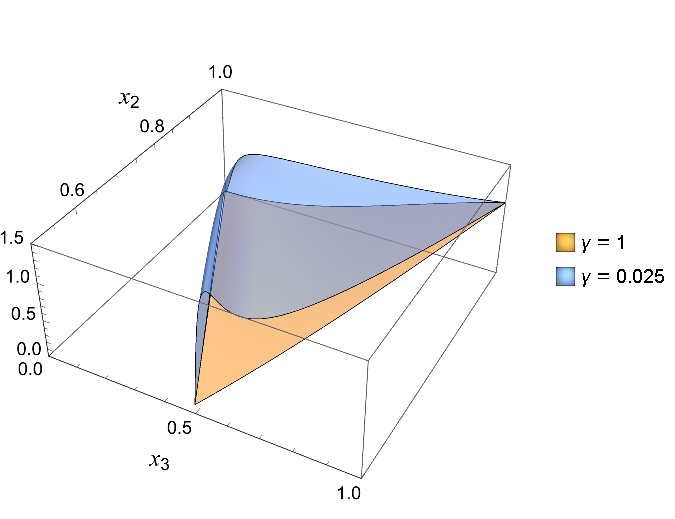
\includegraphics[width=.48\textwidth]{figures/3dintroMink.pdf}}
    \raisebox{-0.5\height}{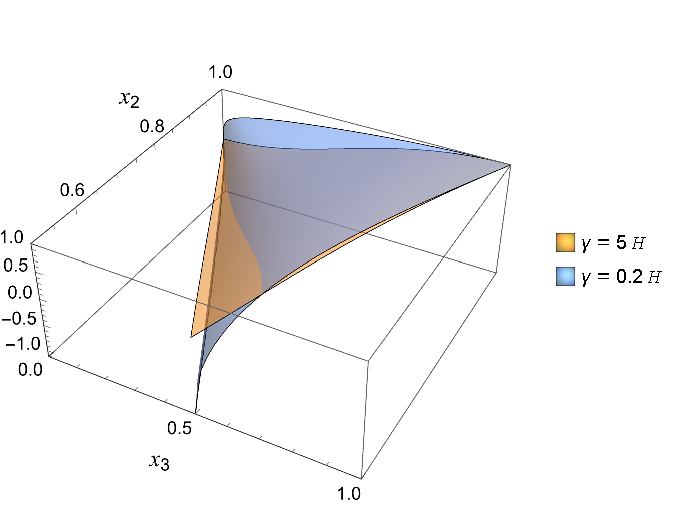
\includegraphics[width=.48\textwidth]{figures/3dintrodS.pdf}}
\end{minipage}
\caption{\label{fig:foldedintro} Minkowski 時空（左）と de Sitter 時空（右）で、演算子 $\pi_a^3$ が生成する接触バイスペクトルの形状関数 $S(x_2,x_3)\equiv(x_2x_3)^2[B(k_1,x_2k_1,x_3k_1)/B(k_1,k_1,k_1)]$。左：バイスペクトルは \Eq{eq:genintro} で与えられ、その特異性は \Eq{eq:singdissipintro} の $\mathrm{Sing}_\gamma$ によって制御される（\Sec{subsec:flatB} を参照）。特異性が解消されるので、どの物理的配置でもバイスペクトルは有限である。散逸パラメータ $\gamma$ が小さくなるにつれ、形状関数は正三角形（橙）から folded（青）へ移る。散逸が小さい領域では等脚 folded 配置の近くで信号が増大する。右：de Sitter 時空でも定性的な特徴は同じである。散逸が大きいとき（橙）は正三角形の配置で最大となり、小さいとき（青）は folded 領域の近くで増大する。図では明瞭でないが、解析的議論によって (i) 散逸が folded 発散を制御すること、(ii) squeezed 極限 $x_3\ll x_2=1$ でも整合関係が成立することが確認される。}
\end{figure}

特異性構造 $\mathrm{Sing}_\gamma$ は、散逸係数 $\gamma$ の大きさによって二つの異なる振る舞いを示す。
\begin{itemize}
\item 強い散逸の領域では、\Eq{eq:singdissipintro} の $3i\gamma/2$ の項が常に支配的となり、信号は $k_1\simeq k_2\simeq k_3$ の\textit{正三角形}の配置で最大になる（\Fig{fig:foldedintro} の橙色の領域）。
\item 弱い散逸の領域では、$k_2+k_3\simeq k_1$ である folded 領域で $\mathrm{Sing}_\gamma$ が小さくなり、信号は主に $k_2\simeq k_3\simeq k_1/2$ の\textit{等脚 folded}\footnote{ここでは、スケール変換を除けば一パラメータ族の配置 $k_1+k_2=k_3$ とその置換である folded 特異性と、スケール変換を除けば単一の運動学的配置 $k_2\simeq k_3\simeq k_1/2$ とその置換である等脚 folded 配置を区別する。}配置で最大になる（\Fig{fig:foldedintro} の青色の領域）。
\end{itemize}
平坦時空を超える場合、完全に一般的な解析結果を得るのは難しく、\Sec{subsec:bispecdS} では主に数値結果を用いる。平坦時空と同様に、強い散逸（$\gamma\gg H$）と弱い散逸（$\gamma\ll H$）で異なる振る舞いが現れる（\Fig{fig:foldedintro} の右パネル）。強い散逸では、\cite{LopezNacir:2011kk} がすでに指摘したように、信号は正三角形の配置で最大になる。弱い散逸では、folded 領域の近くで極値をとる。一見すると、開放ダイナミクスのこの決定的な特徴は、非 Bunch--Davies 初期状態 \cite{Holman:2007na,Chen:2006nt,Meerburg:2009ys,Agullo:2010ws,Ashoorioon:2010xg,Agarwal:2012mq,Ashoorioon:2013eia,Albrecht:2014aga,Green:2020whw} のように、folded 三角形で信号を生むほかの模型と縮退しているように見える。しかし決定的な違いは、散逸がピークを滑らかにし、三角形配置の境界から移動させて発散を正則化するため、任意の物理的配置でバイスペクトルが有限となる点である。特に、バイスペクトルの squeezed 極限 $k_1\simeq k_2\gg k_3$ で発散しないことを意味する。$\gamma/H$ が小さい場合、正則化された folded 特異性による中間的なピークが現れうるが、整合関係 \cite{Maldacena:2002vr,Creminelli:2004yq,Cheung:2007sv,Creminelli:2012ed,Hinterbichler:2012nm,Assassi:2012zq,Pajer:2017hmb,Avis:2019eav} は成立し、理論の対称性によって squeezed 極限はゼロに向かう。

\paragraph{UV 模型と対応付け} インフレーションの開放有効場理論は、局所的で、散逸を伴いうるダイナミクスをもつ、すべての単一時計模型を捉える。明示的な UV 模型の一つが最近 \cite{Creminelli:2023aly} で研究された。\Sec{sec:matching} では、本形式がそのダイナミクスの正確な低エネルギー有効記述となることを示す。この模型は、インフラトン場 $\phi$ に加え、$U(1)$ 対称性が弱く破れた質量のあるスカラー場 $\chi$ を含み、その作用は次式で与えられる。

\begin{align}\label{eq:actionmatchintro}
S= \int \dd^4 x &\sqrt{- g} \bigg[ \frac{1}{2} M_{\mathrm{Pl}}^2  R - \frac{1}{2} \left(\partial \phi \right)^2 - V(\phi) - \left|\partial \chi \right|^2 + M^2 \left| \chi \right|^2 \nonumber \\
- &\frac{\partial_\mu \phi}{f}\left( \chi \partial^\mu \chi^* - \chi^* \partial^\mu \chi\right) - \frac{1}{2}m^2\left(\chi^2 + \chi^{*2}\right)\bigg].
\end{align}

この模型には Hubble 半径より短いスケールで狭い不安定帯があり、そこで粒子生成が起きる。次の非線形 Langevin 方程式

\begin{align}\label{eq:Paolointro}
\pi'' + \left( 2H + \gamma\right)a\pi' - \partial_i^2 \pi &\simeq \frac{\gamma}{2\rho f} \left[ \left( \partial_i \pi\right)^2 - 2 \pi \xi \pi^{\prime2}\right] - \frac{a^2m^2}{f} \left(1+2\pi\xi \frac{\pi'}{a \rho f} \right) \delta \mathcal{O}_S\,,
\end{align}

は \cite{Creminelli:2023aly} で使われたものであり、ここで論じるインフレーションの開放有効場理論との等価性を示す。この UV 模型では、有効理論は次式に帰着する。

\begin{align}\label{eq:Seffmatchintro}
\quad S_{\mathrm{eff}} &= \int \dd^4 x \Big[ a^2 \pi'_{r} \pi'_{a} - c_{s}^{2} a^2 \partial_i \pir  \partial^i \pia   -  a^3 \gamma \pi'_{r} \pia + i \beta_1 a^4 \pia^2 \nonumber \\
+ &\frac{ \left(8\gamma_2 - \gamma\right)}{2f^{2}_{\pi}}  a^2\pir^{\prime2} \pia	+ \frac{\gamma}{2f_{\pi}^{2}} a^2	\left(\partial_i \pir \right)^2 \pia - 2i\frac{\beta_{5}}{f_\pi^2} a^3 \pir^{\prime} \pia^2 +\frac{\delta_1}{f_\pi^2} a^4 \pia^3  \Big]. 
\end{align}

\paragraph{論文の構成} 本論文の残りの部分は以下のように構成される。\Sec{sec:1} では、最初から非結合極限で作業し、単一時計インフレーションの開放有効場理論をボトムアップに構成する。\Sec{sec:Pk} では理論の伝播関数を導き、パワースペクトルを求める。\Sec{sec:bispec} では接触バイスペクトルを計算し、相互作用を摂動的に扱う。最後に \Sec{sec:matching} では、開放 EFT と特定の UV 完成との明示的なマッチングを行う。\Sec{sec:disc} に結論をまとめ、計算の詳細はその後の付録に収める。

\sectionlink{インフレーションの開放有効場理論}\label{sec:1}

開放系を研究する出発点は、記述したい自由度、通常「\textit{系}」と呼ぶものと、観測できないとみなす自由度、通常「\textit{環境}」と呼ぶものを選ぶことである。単一時計インフレーションに注目するため、ここでの系は、まもなく定義する時間並進のゴールドストーン・ボソンと同定されるスカラー場 $\uppi$ とする。環境との相互作用によって非ユニタリな時間発展が生じる状況で、$\uppi$ の EFT を構成したい。ユニタリに発展する純粋状態は、次の波動関数で表せる。

\begin{align}
\Psi\left[\uppi; \eta_0 \right] = \int_{\Omega}^{\uppi} \mathcal{D} \uppi_+ \ee^{i S_{\mathrm{eff}}\left[ \uppi_+\right]},
\end{align}

これはインフレーション研究の多くに共通する出発点であり、場の理論としての波動関数 $\Psi$ は近年精力的に研究されている \cite{Anninos:2014lwa,Arkani-Hamed:2017fdk,Arkani-Hamed:2018kmz,Pajer:2020wnj,Goodhew:2020hob,Cespedes:2020xqq,Goodhew:2021oqg,Melville:2021lst,Salcedo:2022aal,Baumann:2021fxj,Albayrak:2023hie,Stefanyszyn:2023qov,Sleight:2021plv,Celoria:2021vjw,Creminelli:2024cge,Chakraborty:2023yed}（総説と追加文献については \cite{Baumann:2022jpr,Benincasa:2022gtd} を参照）。これに対して混合状態は換算密度行列 $\widehat{\rho}_{\mathrm{red}}$ で記述され、その行列要素は in-in 経路、すなわち\textit{閉時間経路}に沿う経路積分から求められる。in-in 経路を扱う便利な方法は、場を $\uppi_+$ と $\uppi_-$ に二重化することであり、次式が得られる。

\begin{align}
\rho_{\mathrm{red}}\left[\uppi, \uppi';\eta_0\right] = \int_{\Omega}^\uppi \mathcal{D}\uppi_+ \int_{\Omega}^{\uppi'} \mathcal{D}\uppi_- \ee^{i S_{\mathrm{eff}}\left[ \uppi_+, \uppi_-\right]}.\label{eq:densitymatrix}
\end{align}

ここで $\Omega$ は初期状態の選択を表し、原理的には初期の混合密度行列でもよい。以下では、無限の過去において系が Bunch--Davies 状態にあり、$\uppi$ セクターへ縮約しても純粋状態だったと仮定する。有効汎関数 $S_{\mathrm{eff}}$ にはいくつかの寄与がある。第一に、Hermitian な Hamiltonian に従う時間発展の寄与がある。これは経路積分の二つの枝を混ぜない $S_{\mathrm{eff}}$ の相互作用に対応し、一般に $S_\uppi[\uppi_+]-S_\uppi[\uppi_-]$ の形をとる。第二に、エネルギーと情報の損失・流入を符号化する非ユニタリ、すなわち非 Hamiltonian 的な効果がある。これは二つの枝をまたぐ相互作用として現れ、その寄与を表す $S_{\mathrm{eff}}$ の部分を Feynman--Vernon の影響汎関数 $S_{\mathrm{IF}}[\uppi_+,\uppi_-]$ と呼ぶことがある。したがって\textit{開放有効汎関数} $S_{\mathrm{eff}}[\uppi_+,\uppi_-]$ は、次のように Hermitian な部分と非 Hermitian な部分をもつ。

\begin{align}\label{eq:Seffref}
S_{\mathrm{eff}}\left[ \uppi_+, \uppi_-\right] = S_\uppi\left[\uppi_+\right] - S_\uppi\left[\uppi_-\right] + S_{\mathrm{IF}}\left[\uppi_+,\uppi_- \right].
\end{align}

非平衡の開放 EFT に関する最近の研究 \cite{Crossley:2015evo,Boyanovsky:2015xoa,Glorioso:2016gsa,Liu:2018kfw,Hongo:2018ant,Oppenheim:2023izn,Akyuz:2023lsm} を踏まえ、単一時計インフレーションの $S_{\mathrm{eff}}[\uppi_+,\uppi_-]$ を構成し調べることが本研究の目的である。

\subsectionlink{EFT の構成}\label{subsec:EFT}

この節では開放有効汎関数 $S_{\mathrm{eff}}[\uppi_+,\uppi_-]$ に課される一連の条件を導入・検討する。確率保存などの一般原理から従う条件もあれば、スケール階層のある系や単一時計インフレーションの研究に固有の条件もある。

\subsubsectionlink{非平衡条件}

最初の条件は、環境について跡を取った開放量子系が、Hermitian な時間発展をする閉鎖系から得られるという要請に由来する \cite{breuerTheoryOpenQuantum2002,Crossley:2015evo,Glorioso:2016gsa,Liu:2018kfw}。

\begin{align}
S_{\mathrm{eff}} \left[\uppi_+,\uppi_+\right] &= 0\,,  \\
    S_{\mathrm{eff}} \left[\uppi_+,\uppi_-\right] &= - 	S^*_{\mathrm{eff}} \left[\uppi_-,\uppi_+\right] \,, \\
    \Ima S_{\mathrm{eff}} \left[\uppi_+,\uppi_-\right] &\geq 0 \,.
\end{align}

これらの条件は、それぞれ密度行列の定義的性質から従う。
\begin{enumerate}
\item 規格化、$\Tr\widehat{\rho}_{\mathrm{red}}=1$。
\item Hermitian 性、$\widehat{\rho}_{\mathrm{red}}^\dagger=\widehat{\rho}_{\mathrm{red}}$。
\item 正値性、Hilbert 空間の任意の $\ket{\phi}$ に対して $\bra{\phi}\widehat{\rho}_{\mathrm{red}}\ket{\phi}\geq0$。
\end{enumerate}
\cite{Glorioso:2016gsa} に沿った導出は \App{app:deriv} に記す。こうして得られる構造は非摂動的に成立し、特にあらゆる loop 次数で有効である。後で見るように、これらの条件は EFT に入れられる演算子の数を大幅に減らす。

$S_{\mathrm{eff}}[\uppi_+,\uppi_-]$ の項数は場や微分の数とともに急速に増えるため、整理原理を選ぶと便利である。有用な基底\footnote{Hermitian な時間発展は、二つの枝の混合項が存在しないという形で、$+/-$ 基底でもっとも明瞭に表れる。逆に、$r$--$a$ 基底では $\uppi_a$ の場が伝播せず、因果構造が簡単になる \cite{kamenev_2011}。文献では $\uppir\equiv\uppicl$、$\uppia\equiv\uppiq$ という等価な記法も使われる \cite{kamenev_2011,Radovskaya:2020lns}。物理的状況によっては、この「古典・量子」記法は $\hbar$ の次数を数える助けになるが、インフレーションではそうならないため、誤解を招きうるこの名称を避ける。} は \textit{Keldysh 基底}（\textit{遅延・先進基底}とも呼ばれる）で、次式で定義される。

\begin{align}\label{eq:basis}
 \uppi_r &= \frac{\uppi_+ + \uppi_-}{2} \quad \mathrm{and} \quad \uppi_a = \uppi_+ - \uppi_-\, \qquad \Leftrightarrow \qquad  \uppi_\pm =\uppir\pm \frac12 \uppia\,.
\end{align}

この $r$--$a$ 基底では、開放有効汎関数 $S_{\mathrm{eff}}$ の条件は次のようになる。

\begin{align}
S_{\mathrm{eff}} \left[\uppi_r,\uppi_a = 0\right] &= 0 \,,\label{eq:norm} \\
S_{\mathrm{eff}} \left[\uppi_r,\uppi_a\right] &= - 	S^*_{\mathrm{eff}} \left[\uppi_r,-\uppi_a\right] \,,\label{eq:herm} \\
\Ima S_{\mathrm{eff}} \left[\uppi_r,\uppi_a\right] &\geq 0. \label{eq:pos}
\end{align}

\subsubsectionlink{時間並進対称性の破れ}

対称性は EFT 演算子の数と構造をさらに制限する。一般的な考え方は、非平衡系での対称性の破れ方を調べる最近の Schwinger--Keldysh coset 構成 \cite{Akyuz:2023lsm} に基づく。対称群 $G$ の下で不変な微視的理論 $S_{\mathrm{UV}}[\uppi,\chi]$ を考えよう。閉鎖系の Schwinger--Keldysh 作用 $S_{\mathrm{UV}}[\uppi_+,\chi_+]-S_{\mathrm{UV}}[\uppi_-,\chi_-]$ は $G_+\times G_-$ の下で不変である。$\chi$ 場を積分消去すると対称性の破れ方が変わり、$S_{\mathrm{eff}}[\uppi_+,\uppi_-]$ はより小さい部分群 $G_{\mathrm{IR}}$ の下で不変になる。多くの場合、これは $\uppi_+$ と $\uppi_-$ を同時に変換する対角部分群である \cite{Akyuz:2023lsm}。さらに、熱状態における動的 Kubo--Martin--Schwinger（KMS）対称性 \cite{Liu:2018kfw} のような、状態の選択に伴う自発的対称性の破れも考えられる。しかし宇宙論的な環境はしばしば非熱的なので \cite{Colas:2022hlq,Hsiang:2021vgx}、ここでは論じない。

非結合極限の EFToI \cite{Creminelli:2006xe,Cheung:2007st,LopezNacir:2011kk} と同様に、本論文の開放 EFT には自由度が一つだけある。これはインフラトン背景が時間並進を自発的に破ることに伴う Nambu--Goldstone ボソンである。この対称性の破れ方を最初に調べた \cite{Hongo:2018ant} に従う。$\epsilon_+$、$\epsilon_-$ で表され、それぞれ次式のように非線形に実現される独立な時間並進の下で不変な UV 作用を考える。

\begin{align}
        \uppi_+(t) \rightarrow \uppi'_+(t) = \uppi_+(t+\epsilon_+)+\epsilon_+,\quad\quad\uppi_-(t) \rightarrow \uppi'_-(t) = \uppi_-(t+\epsilon_-)+\epsilon_-,  
    \end{align}

追加の環境場には時間並進が線形に作用する。環境について跡を取ると、開放有効汎関数 $S_{\mathrm{eff}}[\uppi_+,\uppi_-]$ は一般に任意の $\epsilon_\pm$ 並進に対して不変ではない。より正確には、次の変換の下では不変性が残る（\Fig{fig:sym} の左パネル）\cite{Hongo:2018ant}。

\begin{align}
        \epsilon_+ = \epsilon_- =\epsilon_{r}\,,
    \end{align}

一方、次の並進は

\begin{align}
        \epsilon_+ =  - \epsilon_- =\frac{\epsilon_{a}}{2}
    \end{align}

明示的に破れる（\Fig{fig:sym} の右パネル）。したがって微視的作用の二つの時間並進対称性から、対角部分群 $\epsilon_+=\epsilon_-$ だけが残る。

\begin{figure}[tbp]
    \centering
    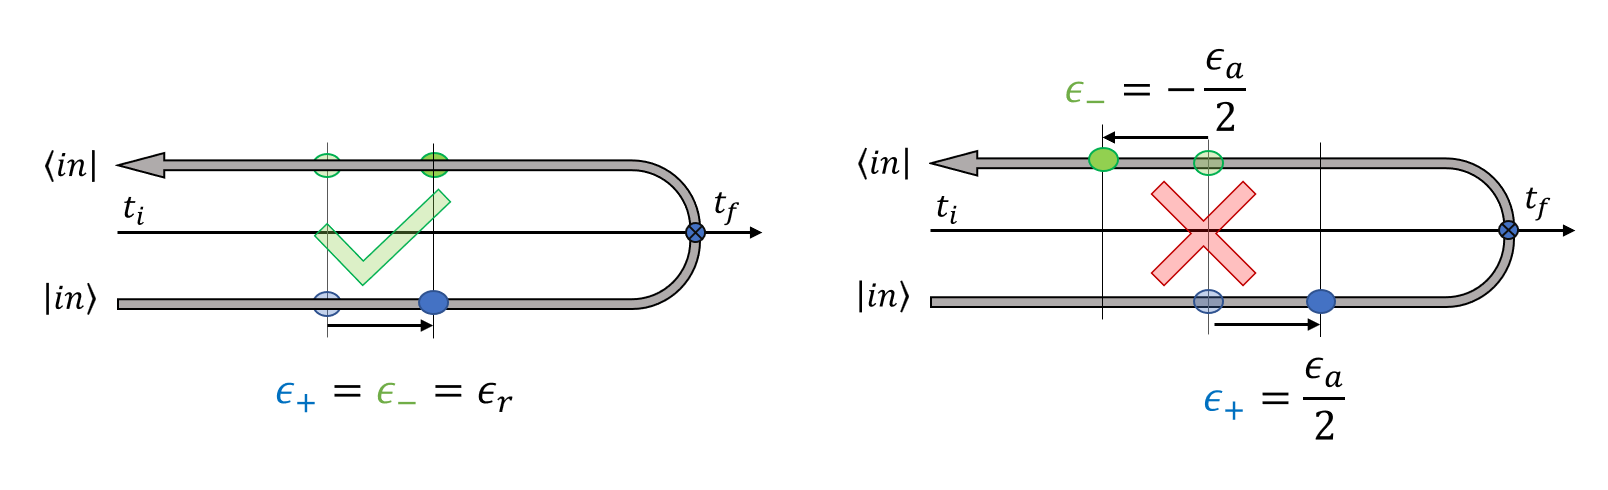
\includegraphics[width=1\textwidth]{figures/sym_ra.png}
\caption{閉時間経路上の $\epsilon_r$ 変換と $\epsilon_a$ 変換。両輪郭とも時間は左から右へ進み、矢印は経路順序を表す（$\ket{in}$ では時間順序、$\bra{in}$ では反時間順序）。$\epsilon_r$ は「$+$」と「$-$」の変数を同じ方向へ移し、$\epsilon_a$ は逆方向へ移す。$\epsilon_r$ 変換は保たれるが、$\epsilon_a$ 変換は散逸効果によって明示的に破れる \cite{Hongo:2018ant}。}
    \label{fig:sym}
\end{figure}

この対角部分群の時間並進と boost の下で $\uppi_r$、$\uppi_a$ がどのように変換するかを考えよう。Keldysh 基底における $\epsilon_r$ 変換は、次のように与えられる \cite{Hongo:2018ant}（\Fig{fig:sym} の左パネル）。\footnote{$S_{\mathrm{eff}}[\uppi_r,\uppi_a]$ が \Eq{eq:translRsym} の変換で不変なことは直接確認できる。具体的には、$\uppi_r$ と $\uppi_a$ を $\epsilon_r$ で展開すると、次のようになる。

\begin{align}\label{eq:translRsymexp}
        \uppi_{r}(t,\bmx) &\rightarrow \uppi_{r}(t,\bmx) + \epsilon_r\left[1+\dot{\uppi}_{r}(t,\bmx)\right] + \mathcal{O}\left[(\epsilon_r)^2\right],\\
        \uppi_{a}(t,\bmx) &\rightarrow  \uppi_{a}(t,\bmx) + \epsilon_r\dot{\uppi}_{a}(t,\bmx) + \mathcal{O}\left[(\epsilon_r)^2\right].
\end{align}

}

\begin{align}\label{eq:translRsym} 
    \uppi_{r}(t,\bmx) \rightarrow \uppi'_{r}(t,\bmx) &= \uppi_{r}(t+\epsilon_{r},\bmx) + \epsilon_{r},\\
    \uppi_{a}(t,\bmx) \rightarrow \uppi'_{a}(t,\bmx) &= \uppi_{a}(t+\epsilon_{r},\bmx),
\end{align}

一方、$\Lambda_r$ 変換は次式に従う。

\begin{align}\label{eq:LorentzRsym}
\uppi_{r}(t,\bmx) \rightarrow \uppi'_{r}(t,\bmx) &= \uppi_{r}\left(\Lambda^0_{r~\mu}x^\mu,\Lambda^i_{r~\mu}x^\mu \right)+\Lambda^0_{r~\mu}x^\mu - t, \\
\uppi_{a}(t,\bmx) \rightarrow \uppi'_{a}(t,\bmx) &= \uppi_{a}\left(\Lambda^0_{r~\mu}x^\mu,\Lambda^i_{r~\mu}x^\mu \right),
\end{align}

ここで $\Lambda^\mu_{r~\nu}\in\mathrm{SO}(1,3)$ とした。重要なのは、$\uppi_r$ が\textit{時間並進と boost を非線形に実現する}のに対し、$\uppi_a$ は通常の物質場と同じく\textit{線形に変換する}という点である \cite{Hongo:2018ant}。

\subsubsectionlink{局所性}

ここでは $S_{\mathrm{eff}}$ の時間・空間における\textit{局所性}を論じる。もっとも一般的な場合、環境について跡を取ると、厳密な UV 完成を知らなければ扱えない、複雑な非局所有効汎関数が生じる。しかし標準的な EFT と同様に、\textit{スケールの分離}があれば大幅な簡略化が起きる。本論文では、まさにこの可能性に焦点を当てる。環境を特徴付ける典型的な長さ・時間スケールが、宇宙論的相関関数を計算する Hubble 時間・Hubble 半径よりはるかに短いと想定する。この階層によって、開放 EFT は時空で局所的となる。つまり、同じ時空点における場と、その有限個だが任意の階数の微分の積からなる演算子で構成される。すべての UV 模型にこの階層があるわけではない。例えば、$\phi F\tilde F$ 結合がゲージモードのタキオン的生成を引き起こす、よく研究されたインフレーション模型 \cite{Anber:2009ua} では、ゲージ場が主に Hubble 半径通過の前後で生成されるので、$\uppi$ の開放 EFT は非局所的になる。開放 EFT が非局所的、または非 Markov 的になりうる別の例は \cite{breuerColloquiumNonMarkovianDynamics2016,Prudhoe:2022pte,Shandera:2017qkg,Colas:2022hlq,Colas:2022kfu,Colas:2024xjy} を参照。このような模型を本論文の開放 EFT で記述できないことは、開放系に固有の新しい問題ではない。極めて軽い場や無質量場を積分消去しようとすれば、標準的な EFT でも同じことが起きる。

そこでスケール階層をもつ模型に注目する。そのような模型の一つが最近 \cite{Creminelli:2023aly} で構成・詳しく研究された。\Sec{sec:matching} で述べるように、その UV 完成に本論文の EFT 記述を対応付けることができた。局所性の物理的な意味は \Sec{sec:disc} でも論じる。

局所的な開放 EFT を動機付けたので、次に非平衡条件と対称性に整合するすべての局所演算子を書き下したい。不変な組合せを基本構成要素に使えばよい \cite{Akyuz:2023lsm}。開放有効汎関数は $\uppi_a$、$t+\uppi_r$、それらの微分 $\partial_\mu\uppi_a$、および

\begin{align}\label{eq:Pmu}
    P_\mu = \partial_\mu (t + \uppi_{r}) = \delta^0_{~\mu}+ \partial_\mu \uppi_{r}
\end{align}

から構成できる。これは通常の EFToI \cite{Hongo:2018ant} の場合と同様である。微分展開の主要次数で作業し、各場につき高々一階の微分をもつ演算子に制限する。最後に、\cite{LopezNacir:2011kk} に従い、スローロール補正を除いて $\uppi$ が唯一の動的自由度となる非結合極限で作業する。環境があってもこの記述は有効である（\cite{LopezNacir:2011kk} の付録 D を参照）。元の導出 \cite{Cheung:2007st} と同様に、ユニタリ・ゲージから始め、空間微分同相変換には不変だが時間微分同相変換には不変でない重力理論を指定して、開放 EFToI を導くことも考えられる。計量摂動の次数ごとに行うのは容易だが、場を二重化したとき、重力の非摂動的で微分同相不変な構造をどう整理するかは明らかでない。例えば、添字を共変化するために $g^+_{\mu\nu}$、$g^-_{\mu\nu}$ やその組合せを用いる選択肢が無数にあるように見える。この問題は今後の研究に委ねたい。

\subsectionlink{開放系の有効汎関数}

次に、非平衡条件と上記の対称性に整合し、各場につき高々一階の微分を含む、もっとも一般的な局所開放有効汎関数を書き下す。微分展開に加えて、$\uppi_a$のべきで整理すると便利である。$S_{\mathrm{eff}}=\int\dd^4x\sqrt{-g}\,\mathcal{L}_{\mathrm{eff}}$と書くと、

\begin{align}\label{eq:expref}
    \mathcal{L}_{\mathrm{eff}} = \sum_{n=1}^\infty \mathcal{L}_n\quad\mathrm{with}\quad \mathcal{L}_n = \mathcal{O}(\uppi_{a}^n)
\end{align}

ここではユニタリ性の条件\eqref{eq:norm}から、$\mathcal{L}_{\mathrm{eff}}$が$\uppi_a$に関して一次から始まることを用いた。ただし、$\uppi_a$の高次の演算子が抑制されると主張しているわけではなく、この文脈で一般には正当化されない$\hbar$展開を用いているわけでもない\cite{Radovskaya:2020lns}。多数の異なる項を整理するために$\uppi_a$のべきを利用するだけである。実際の応用のため三次の演算子までに制限し、$\mathcal{L}_1$、$\mathcal{L}_2$、$\mathcal{L}_3$に焦点を当てて一般的な手順を示す。次の次数は少なくとも$\uppi_a$の四次となる。

\paragraph{全微分について} 明示的な構成に入る前に、議論を大きく簡単にする全微分の扱いを説明する\cite{Hongo:2018ant}。インフレーションでは共形時刻$\eta\in(-\infty,0]$を使うため、部分積分（IBP）によって境界項が生じ\cite{Salcedo:2022aal,Braglia:2024zsl}、平坦時空ほど無害ではないかもしれない。この問題を避ける一つの方法は部分積分をしないことだが、本論文の開放EFTで問題がどう現れるかを、通常のEFToIと比べてみよう。in-in経路積分の境界条件により、境界では$\uppi_a=0$である。したがって$\uppi_a$に比例する境界項はすべて消える。消えない境界項には、$\uppi_a$に作用する時間微分が少なくとも一つ必要であり、バルクでは場に二階以上の微分が作用する演算子に対応する。主要次数のEFT演算子に注目する本研究では、これらを無視している。このため全微分を安全に捨てられる。

\subsubsectionlink{ゴールドストーン・ボソンの有効汎関数}

以上の原理に従い、$\uppi_a$の次数ごとに$\mathcal{L}_n$を構成する。

\paragraph{$\mathcal{L}_1$汎関数}

まず$\mathcal{L}_1$を例に手順を示そう。\Eq{eq:Pmu}付近で定義した構成要素から、$\uppi_a$に線形な不変量を作る。可能なのは、$\uppi_a$と$P^\mu\partial_\mu\uppi_a=(-\dot{\uppi}_a+\partial^\mu\uppi_r\partial_\mu\uppi_a)$を、次の量のべきに掛けることだけである。

\begin{align}
        \left( P_\mu P^\mu  +1\right) = -2 \dot{\uppi}_{r} + \left( \partial_\mu \uppi_{r}\right)^2,
    \end{align}

この結果、次式を得る\cite{Hongo:2018ant}。\footnote{$\upgamma_n$項の前の符号は、後の便宜のために選んでいる。}

\begin{align}
        \mathcal{L}_1 = & \sum_{n=0}^\infty \left( P_\mu P^\mu  +1\right)^{n} \left[ \upgamma_n \uppi_{a} -\upalpha_n P^\mu \partial_\mu \uppi_{a}  \right].
    \end{align}

EFT係数$\upgamma_n$と$\upalpha_n$は一般には$t+\uppi_r$の関数であり、複素共役に関する条件\eqref{eq:herm}により実数でなければならない。スローロール領域では、主要次数でEFT係数を時間に依存しないものとしてよい\cite{Hongo:2018ant}。

\begin{tcolorbox}[enhanced,breakable,skin first=enhanced,skin middle=enhanced,skin last=enhanced,before upper={\parindent15pt},]{}
\paragraph{背景の時間発展とタドポール}

揺らぎのダイナミクスに進む前に、タドポールの相殺\cite{Cheung:2007st,Collins:2012nq}を論じ、標準的なEFToIの背景の時間発展との関係を確認する。\Eq{eq:expref}の下で述べたように、ユニタリ性の条件\eqref{eq:norm}により$\mathcal{L}_{\mathrm{eff}}$は$\uppi_a$の一次から始まる。したがって可能なタドポールは次だけである\cite{LopezNacir:2011kk,Hongo:2018ant}。

\begin{align}\label{eq:tad1}
            S_{\mathrm{eff}}  \supset  \int \dd^4 x  \sqrt{-g} \left[ \upgamma_0(t) \uppi_a  + \upalpha_0(t) \dot{\uppi}_a \right],
\end{align}

その相殺条件は次のようになる。

\begin{align}
           - \upgamma_0 + \dot{\upalpha}_0 + 3H \upalpha_0 = 0.
        \end{align}

通常の構成と比べよう。標準的なEFToIでは、次の作用からFLRW背景の時間発展を得る。

\begin{align}\label{eq:SEFToI}
            S_{\mathrm{EFToI}} = \int \dd^4x \sqrt{-g} \left[\frac{1}{2} M_{\mathrm{Pl}}^2 R - \Lambda(t) - c(t) g^{00} \right]
        \end{align}

計量の$g^{00}$成分と$g^{ii}$成分で変分すると、

\begin{align}\label{comb1}
            3 M_{\mathrm{Pl}}^2  H^2 &= c(t) + \Lambda(t)\,, \\
            - M_{\mathrm{Pl}}^2 \dot{H} &= c(t). \label{comb2}
        \end{align}

St\"uckelbergの方法で$t\rightarrow t+\uppi$として微分同相不変性を再導入し、\Eq{eq:SEFToI}の作用を$\uppi$で変分することもできる。すると、次のタドポール相殺条件が得られる\cite{Cheung:2007st}。

\begin{align}\label{eq:tad2}
            \dot{\Lambda} + \dot{c} + 6 H c = 0\,.
        \end{align}

これは新しい方程式ではなく、\Eqs{comb1}と\eqref{comb2}を組み合わせたものにすぎない。Einstein方程式が全エネルギー運動量テンソルの保存$\nabla^\mu T_{\mu\nu}=0$を意味するため、これは当然である。Keldysh基底へ回転すると、上記二つのタドポールは次のようになる。\footnote{これらの項がユニタリであることは明白である。$\Ddot{\Lambda}\uppi_r\uppi_a$のようなスローロールで抑制される項も考慮すれば、\Sec{subsubsec:unit}で述べるユニタリ性の検査を満たす。}

\begin{align}
              -\left.\Lambda(t)\right|_{t\rightarrow t + \uppi_r + \frac{\uppi_a}{2}} + \left.\Lambda(t)\right|_{t\rightarrow t + \uppi_r - \frac{\uppi_a}{2}}  &= - \dot{\Lambda}(t) \uppi_a + \mathcal{O}(\uppi_a^2),
        \end{align}

および

\begin{align}
            &-\left.c(t) g^{00}\right|_{t\rightarrow t + \uppi_r + \frac{\uppi_a}{2}} + \left.c(t) g^{00}\right|_{t\rightarrow t + \uppi_r - \frac{\uppi_a}{2}}    =  \dot{c}(t) \uppi_a + 2 c(t) \dot{\uppi}_a + \mathcal{O}(\uppi_a^2).
        \end{align}

次のように同定すれば、

\begin{align}\label{eq:tadpole}
            \upalpha_0(t) \equiv 2 c(t) \qquad \mathrm{and} \qquad \upgamma_0 (t)\equiv  \dot{c}(t) - \dot{\Lambda}(t),
        \end{align}

\Eqs{eq:tad1}と\eqref{eq:tad2}は等価になる。
\end{tcolorbox}

以上の議論から得られる主な物理的帰結は次のとおりである。\cite{LopezNacir:2011kk}で指摘されたように、この種の局所的で散逸的なインフレーション模型には新しいタドポールはない。背景の時間発展は葉層の選択によって固定され、全体のエネルギー密度を調べる。そこではインフラトンと未知の環境の寄与は区別されない。\footnote{背景のダイナミクスから系と環境を区別できる葉層が存在するかどうか、例えば異なる荷によって区別できるかどうかを、さらに調べることは興味深い。}系と環境の区別が重要になるのは揺らぎのレベルだけである。そこで初めて、流体力学的方向$\uppi$に対応する観測可能な自由度と、積分消去された観測不能な自由度を分けられる。

背景のダイナミクスを固定し、タドポールを除いたので、$\mathcal{L}_1$は次の明示的な形をとる。

\begin{align}
        \mathcal{L}_1 = - \upalpha_0 \partial^\mu \uppi_{r} \partial_\mu \uppi_{a} &-\sum_{n=1}^\infty \upalpha_n \left[-2 \dot{\uppi}_{r} + \left( \partial_\mu \uppi_{r}\right)^2\right]^{n}\left(-\dot{\uppi}_{a} + \partial^\mu \uppi_{r} \partial_\mu \uppi_{a}\right) \nonumber \\
        +& \sum_{n=1}^\infty \upgamma_n \left[-2 \dot{\uppi}_{r} + \left( \partial_\mu \uppi_{r}\right)^2\right]^n\uppi_{a}.
    \end{align}

二次の$\uppi$項を与え、ゴールドストーン・モードの分散関係に関係するのは$\upalpha_0$、$\upalpha_1$、$\upgamma_1$だけである\cite{Hongo:2018ant}。$\upalpha_0$項はKeldysh基底で書いた通常の運動項であり、基底変換\eqref{eq:basis}から確認できる。前述のタドポール相殺から$\upalpha_0(t)=2c(t)=2M_{\mathrm{Pl}}^2|\dot H|$が得られる。$\upalpha_1$項は非自明な音速を生み、正三角形型の非ガウス性を制御する高次演算子を伴う\cite{Cheung:2007st}。これに対し$\upgamma_1$項にはユニタリな対応物がなく、\Sec{sec:matching}で見るように$\uppi_r$の運動方程式に散逸項を与える。興味深いことに、散逸項$\dot{\uppi}_r\uppi_a$には三次相互作用$(\partial_\mu\uppi_r)^2\uppi_a$が伴い\cite{LopezNacir:2011kk}、その組合せはLorentz boostの下で不変になる。

二次および三次の寄与を明示しよう。$\uppi_a$のべきによる展開に加え、次のように分類できる。

\begin{align}
        \mathcal{L}_{\mathrm{eff}} = \sum_{n,m=1}^\infty  \mathcal{L}^{(m)}_n \quad\mathrm{with}\quad \mathcal{L}^{(m)}_n = \mathcal{O}(\uppi^m,~\uppi_{a}^n,~ \uppi_r^{m-n})
    \end{align}

ここで$m$は場の演算子の数を表す。二次の寄与は次である。

\begin{align}
        \mathcal{L}_1^{(2)} &= \left( \upalpha_0 -2 \upalpha_1\right) \dot{\uppi}_{r} \dot{\uppi}_{a} - \upalpha_0 \partial_i \uppi_{r}  \partial^i \uppi_{a} - 2 \upgamma_1  \dot{\uppi}_{r} \uppi_a
    \end{align}

$\upalpha_0$と$\upalpha_1$は非自明な音速をもつユニタリな運動項を制御し、$\upgamma_1$は系から環境への線形散逸を表す。三次では$\mathcal{L}_1$は次のようになる。

\begin{align}\label{eq:cubicinter}
        \mathcal{L}_1^{(3)} =  &\left(4 \upalpha_2 -3\upalpha_1 \right) \dot{\uppi}^2_{r} \dot{\uppi}_{a} + \upalpha_1 \left(\partial_i \uppi_{r} \right)^2 \dot{\uppi}_a + 2 \upalpha_1  \dot{\uppi}_{r}	\partial_i \uppi_{r}  \partial^i \uppi_{a} \Big.\nonumber \\
        &\qquad + \left(4 \upgamma_2 -\upgamma_1 \right)  \dot{\uppi}^2_{r} \uppi_{a}	+ \upgamma_1 	\left(\partial_i \uppi_{r} \right)^2 \uppi_a 
    \end{align}

第1行はユニタリな演算子$\dot{\uppi}^3$と$(\partial_i\uppi)^2\dot{\uppi}$の一部に対応する。第2行は、\cite{LopezNacir:2011kk}で論じられたように、非線形に実現された対称性によって生じる非線形散逸に対応する。

\paragraph{$\mathcal{L}_2$汎関数}

\cite{Hongo:2018ant}に従い、$\uppi_a$の二次である$\mathcal{L}_2$を構成する。上と同様に、高々一階の微分をもつ演算子を用い、スローロール極限を取ると次式を得る。

\begin{align}\label{eq:diffquad}
    \mathcal{L}_2 &= i \Big[\upbeta_1 \uppi_{a}^2 + \upbeta_2 \left( \partial_\mu \uppi_{a}\right)^2 +\upbeta_3 \left(-\dot{\uppi}_{a} + \partial^\mu \uppi_{r} \partial_\mu \uppi_{a}\right)\uppi_{a} +\upbeta_4 \left(-\dot{\uppi}_{a} + \partial^\mu \uppi_{r} \partial_\mu \uppi_{a}\right)^2 + \cdots \Big]
\end{align}

第3項と第4項は、それぞれ$P^\mu\partial_\mu\uppi_a\uppi_a$と$(P^\mu\partial_\mu\uppi_a)^2$から得られる。省略記号は、最初の四項に$(P^\mu P_\mu+1)=-2\dot{\uppi}_r+(\partial_\mu\uppi_r)^2$の任意のべきを掛けて得られる高次項を表す。作用には少なくとも$\uppi_a$の二次が含まれるため、タドポールの寄与はない。前の$i$は複素共役に関する条件\eqref{eq:herm}から直接従う。$\upbeta_1$に比例する項はLangevin方程式に現れる標準的なノイズ項である（\Sec{sec:matching}）。一方、$\upbeta_2$と$\upbeta_4$の項には$(\partial_\mu\uppi_a)^2$や$\dot{\uppi}_a^2$のような微分補正があり、ノイズをスケール依存にする。

$\upbeta$係数には、$\Ima S_{\mathrm{eff}}[\uppi_r,\uppi_a]\geq0$を要求する\Eq{eq:pos}から正値性の条件が課される。平坦時空で、$\omega^2,k^2\ll|\upbeta_1/\upbeta_{2,4}|$を意味する微分展開を用いると、\cite{Hongo:2018ant}の著者らは$\mathcal{L}_2$では$\upbeta_1$が優勢と結論した（$\upbeta_3$の二次項は全微分として除去できる）。その結果、正値性の条件は

\begin{align}
    \upbeta_1 > 0.
\end{align}

\Sec{sec:Pk}では、パワースペクトルの正値性から、別の観点で同じ条件が現れることを見る。この別の要請は$\upbeta_2$と$\upbeta_4$にも制約を与える。ノイズ核の正値性は、この演算子に$(P^\mu P_\mu+1)=-2\dot{\uppi}_r+(\partial_\mu\uppi_r)^2$の高いべきを掛けたときの非ガウス信号にも直接影響する。

$\uppi_a$の奇数べきについてはWilson係数が実数であれば$\Ima S_{\mathrm{eff}}[\uppi_r,\uppi_a]\geq0$を満たしやすいように見えるが、偶数べきではそれほど単純でない。偶数べきには、正定値でも全微分でもない演算子の組合せが存在するかもしれない。高階微分演算子まで含めても、これまでそのような項は見つかっておらず、原理的には$\uppi_a$の偶数べきの有界性が保証される可能性がある。第二の懸念は、$\uppi_r$を含む非線形相互作用である。もっとも単純なノイズ項$i\upbeta_1\uppi_a^2$に$(P^\mu P_\mu+1)=-2\dot{\uppi}_r+(\partial_\mu\uppi_r)^2$を掛けても、同様に許される演算子になる。三次項$\dot{\uppi}_r\uppi_a^2$は有界でないため、収束を保証するには非ユニタリな摂動性の制約を課す必要がある。

上と同様に、$\mathcal{L}_2$の二次・三次の寄与を明示しよう。三つの二次ノイズは次式で制御される。

\begin{align}
\mathcal{L}_2^{(2)} &= i \left[\upbeta_1 \uppi_a^2 - \left(\upbeta_2 - \upbeta_4\right)\dot{\uppi}_a^2 + \upbeta_2 \left(\partial_i \uppi_{a} \right)^2\right]\,,\label{eq:piq2free}
\end{align}

ここでは二次の$\upbeta_3$に関係する全微分を除いた。三次では次式を得る。

\begin{align}\label{eq:cubicinter2}
\mathcal{L}_2^{(3)} &= i \Big[-(\upbeta_3 -2 \upbeta_7)\dot{\uppi}_{r} \dot{\uppi}_{a} \uppi_a + \upbeta_3 \partial_i \uppi_{r}  \partial^i \uppi_{a} \uppi_a +2 (\upbeta_4+\upbeta_6 - \upbeta_8) \dot{\uppi}_{r} \dot{\uppi}_a^2 \nonumber \\
& \qquad \quad - 2 \upbeta_4   \partial_i \uppi_{r}  \partial^i \uppi_{a} \dot{\uppi}_{a} - 2\upbeta_5 \dot{\uppi}_{r} \uppi_a^2  - 2 \upbeta_6 \dot{\uppi}_{r}(\partial_i\uppi_a)^2\Big],
\end{align}

ここでWilson係数$\upbeta_5$、$\upbeta_6$、$\upbeta_7$、$\upbeta_8$を導入した。これらは\Eq{eq:diffquad}の省略記号に含まれる高次演算子に対応し、\Eq{eq:diffquad}の最初の四項に$(P^\mu P_\mu+1)=-2\dot{\uppi}_r+(\partial_\mu\uppi_r)^2$を掛けて得られる。これらの項の物理的解釈は\Sec{subsubsec:unit}で論じる。

\paragraph{$\mathcal{L}_3$汎関数}

同じ構成を続けて$\mathcal{L}_3$を得られる。

\begin{align}
        \mathcal{L}_3 &= \updelta_1 \uppi_a^3 + \updelta_2 (\partial_\mu \uppi_a)^2 \uppi_a + \updelta_3 \left(-\dot{\uppi}_{a} + \partial^\mu \uppi_{r} \partial_\mu \uppi_{a}\right) \uppi_a^2 + \updelta_4 \left(-\dot{\uppi}_{a} + \partial^\mu \uppi_{r} \partial_\mu \uppi_{a}\right) (\partial_\nu \uppi_a)^2 \Big.  \nonumber\\
        &\qquad \qquad + \updelta_5 \left(-\dot{\uppi}_{a} + \partial^\mu \uppi_{r} \partial_\mu \uppi_{a}\right)^2 \uppi_a  + \updelta_6 \left(-\dot{\uppi}_{a} + \partial^\mu \uppi_{r} \partial_\mu \uppi_{a}\right)^3 + \cdots,
    \end{align}

$\updelta_3$項は$(P^\mu\partial_\mu\uppi_a)\uppi_a^2$から、$\updelta_4$項は$(P^\mu\partial_\mu\uppi_a)(\partial_\nu\uppi_a)^2$から、$\updelta_5$項は$(P^\mu\partial_\mu\uppi_a)^2\uppi_a$から、$\updelta_6$項は$(P^\mu\partial_\mu\uppi_a)^3$から生じる。上と同様に、省略記号は最初の各項に$(P^\mu P_\mu+1)=-2\dot{\uppi}_r+(\partial_\mu\uppi_r)^2$の任意のべきを掛けて得られる高次項を表す。後で見るように、これらの項の解釈には曖昧さがある。$\mathcal{L}_1$からの寄与との関係に応じて、ユニタリな演算子にも非ユニタリな演算子にも対応しうるためである。そこで\Sec{subsubsec:unit}ではこれらを分類する。

$\mathcal{L}_3$の二次・三次の寄与を明示しよう。少なくとも$\uppi_a$の三次であるため、二次の寄与はない。三次に制限すると次式となる。

\begin{align}
        \mathcal{L}_3^{(3)} &=\updelta_1 \uppi_a^3 + (\updelta_5- \updelta_2)  \dot{\uppi}_{a}^2 \uppi_a  + \updelta_2  (\partial_i \uppi_{a})^2 \uppi_a - \updelta_4  (\partial_i \uppi_{a})^2 \dot{\uppi}_a + (\updelta_4-\updelta_6)\dot{\uppi}_{a}^3 ,
    \end{align}

$\updelta_3$の三次の寄与は全微分である。

\begin{tcolorbox}[enhanced,breakable,skin first=enhanced,skin middle=enhanced,skin last=enhanced,before upper={\parindent15pt},]{}
\paragraph{まとめ}

\Sec{subsec:EFT}の仮定の下で、全微分を除いたもっとも一般的な二次の開放有効汎関数は次である。

\begin{align}\label{eq:L2ref}
    &\qquad \mathcal{L}^{(2)} =\left( \upalpha_0 -2 \upalpha_1\right) \dot{\uppi}_{r} \dot{\uppi}_{a} - \upalpha_0 \partial_i \uppi_{r}  \partial^i \uppi_{a} \nonumber   \\
    &- 2 \upgamma_1  \dot{\uppi}_{r} \uppi_a+i \left[\upbeta_1 \uppi_a^2 - \left(\upbeta_2 - \upbeta_4\right)\dot{\uppi}_a^2 + \upbeta_2 \left(\partial_i \uppi_{a} \right)^2\right],
\end{align}

EFT係数は\cite{Hongo:2018ant}の記法に合わせた。第1行は運動項と有効音速をもつ通常のユニタリなダイナミクスに対応する。第2行の$\upgamma_1$で制御される最初の項は、周囲の環境に起因する散逸を表す。残りの$\upbeta_i$係数は、拡散、すなわちノイズが誘起する過程を制御する。\footnote{環境が熱平衡に従う場合、KMS対称性は$\upgamma_i$と$\upbeta_j$の間に関係を課す\cite{Liu:2018kfw}。}

三次では、全微分を除いたもっとも一般的な開放有効汎関数は次のように書ける。

\begin{align}
    \mathcal{L}^{(3)} &= \left(4 \upalpha_2 -3\upalpha_1 \right) \dot{\uppi}^2_{r} \dot{\uppi}_{a} + \upalpha_1 \left(\partial_i \uppi_{r} \right)^2 \dot{\uppi}_a + 2 \upalpha_1  \dot{\uppi}_{r}	\partial_i \uppi_{r}  \partial^i \uppi_{a} \Big. \label{eq:L13} \\
    &\qquad \quad + \left(4 \upgamma_2 -\upgamma_1 \right)  \dot{\uppi}^2_{r} \uppi_{a}	+ \upgamma_1 	\left(\partial_i \uppi_{r} \right)^2 \uppi_a \nonumber \\ 
    +&i \Big[-(\upbeta_3 -2 \upbeta_7)\dot{\uppi}_{r} \dot{\uppi}_{a} \uppi_a + \upbeta_3 \partial_i \uppi_{r}  \partial^i \uppi_{a} \uppi_a +2 (\upbeta_4+\upbeta_6 - \upbeta_8) \dot{\uppi}_{r} \dot{\uppi}_a^2 \label{eq:L23} \\
    & \qquad \quad - 2 \upbeta_4   \partial_i \uppi_{r}  \partial^i \uppi_{a} \dot{\uppi}_{a} - 2\upbeta_5 \dot{\uppi}_{r} \uppi_a^2  - 2 \upbeta_6 \dot{\uppi}_{r}(\partial_i\uppi_a)^2\Big] \nonumber \\
    +&\updelta_1 \uppi_a^3 + (\updelta_5- \updelta_2)  \dot{\uppi}_{a}^2 \uppi_a  + \updelta_2  (\partial_i \uppi_{a})^2 \uppi_a - \updelta_4  (\partial_i \uppi_{a})^2 \dot{\uppi}_a + (\updelta_4-\updelta_6)\dot{\uppi}_{a}^3, \label{eq:L33}
\end{align}

式\ref{eq:L13}は$\mathcal{L}_1^{(3)}$から、式\ref{eq:L23}は$\mathcal{L}_2^{(3)}$から、式\ref{eq:L33}は$\mathcal{L}_3^{(3)}$から得られる。

\end{tcolorbox}

de Sitter時空で共形時刻を使い、$a=-1/(H\eta)$とすると、三次までの開放有効汎関数は次のようになる。

\begin{align}
&\quad S_{\mathrm{eff}}^{(2)} = \int \dd^4 x \Big\{\left( \upalpha_0 -2 \upalpha_1\right) a^2 \uppi'_{r} \uppi'_{a} - \upalpha_0 a^2 \partial_i \uppi_{r}  \partial^i \uppi_{a}   \\
-& 2 a^3 \upgamma_1 \uppi'_{r} \uppi_a + i \left[\upbeta_1 a^4 \uppi_a^2 - \left(\upbeta_2 - \upbeta_4\right) a^2\uppi_a^{\prime2} + \upbeta_2 a^2 \left(\partial_i \uppi_{a} \right)^2\right] \Big\}, \nonumber
\end{align}

および

\begin{align}
S_{\mathrm{eff}}^{(3)} =  \int &\dd^4 x \Big\{\left(4 \upalpha_2 -3\upalpha_1 \right) a \uppi_r^{\prime2} \uppi'_{a} + \upalpha_1 a \left(\partial_i \uppi_{r} \right)^2 \uppi'_a + 2 \upalpha_1 a \uppi'_{r}	\partial_i \uppi_{r}  \partial^i \uppi_{a} \\
& \qquad \quad + \left(4 \upgamma_2 -\upgamma_1 \right)  a^2\uppi_r^{\prime2} \uppi_{a}	+ \upgamma_1 a^2	\left(\partial_i \uppi_{r} \right)^2 \uppi_a \nonumber \Big. \\
&+ i \Big[-(\upbeta_3-2\upbeta_7) a^2 \uppi'_{r} \uppi'_{a} \uppi_a + \upbeta_3 a^2 \partial_i \uppi_{r}  \partial^i \uppi_{a} \uppi_a +2 (\upbeta_4+\upbeta_6 - \upbeta_8) a \uppi'_{r} \uppi_a^{\prime2} \nonumber \\
& \qquad \quad - 2 \upbeta_4  a \partial_i \uppi_{r}  \partial^i \uppi_{a} \uppi'_{a} - 2\upbeta_5 a^3 \uppi_r^{\prime} \uppi_a^2  - 2 \upbeta_6 a \uppi_r^{\prime} (\partial_i\uppi_a)^2 \Big] \nonumber\\
&+\updelta_1 a^4 \uppi_a^3 + (\updelta_5- \updelta_2) a^2 \uppi_a^{\prime2} \uppi_a  + \updelta_2 a^2 (\partial_i \uppi_{a})^2 \uppi_a - \updelta_4 a  (\partial_i \uppi_{a})^2 \uppi'_a + (\updelta_4-\updelta_6) a \uppi_a^{\prime3} \Big\}. \nonumber
\end{align}

\subsubsectionlink{EFT演算子の分類}\label{subsubsec:unit}

上の構成では、ユニタリな場合と比べて多様な項が現れる。標準的なEFToI\cite{Cheung:2007st}では$\mathcal{L}^{(2)}$に自由パラメータは一つだけだが、ここでは五つある。$\mathcal{L}^{(3)}$では\cite{Cheung:2007st}の一つに対して十三ある。追加の自由度による真の非ユニタリ効果を記述する演算子もあれば、ユニタリな相互作用をKeldysh基底で書いたために現れるだけの演算子もある。ここでは両者を区別する手順を構築する。

\paragraph{EFToIの回復} 本研究は未知の環境と相互作用する$\pi$の非結合極限を扱う。したがって、開放有効汎関数$S_{\mathrm{eff}}$は、ある極限でEFToI\cite{Cheung:2007st}を再現しなければならない。この極限が理論のパラメータ空間におけるユニタリ方向を定める。まず、Keldysh基底で次のように書かれるEFToIの二次項を考える。

\begin{equation}
\frac{1}{2}\left[\dot{\uppi}_{+}^{2}-c_{s}^{2}(\partial_{i}\uppi_{+})^{2}\right]-\frac{1}{2}\left[\dot{\uppi}_{-}^{2}-c_{s}^{2}(\partial_{i}\uppi_{-})^{2}\right]=\dot{\uppi}_r\dot{\uppi}_a-c_{s}^{2}\partial_{i}{\uppir}\partial_{i}{\uppia}.
\end{equation}

これは次の条件の下で\Eq{eq:L2ref}の第1行と一致する。

\begin{equation}
c_{s}^{2} = \frac{\upalpha_0}{\upalpha_{0}-2\upalpha_1}.
\end{equation}

次にEFToIの三次演算子を考える。$\dot{\uppi}^3$から始めると、Keldysh基底でのユニタリな相互作用は次式となる。

\begin{equation}\label{eq:Unitarypiq3}
\dot{\uppi}^{3}_{+}-\dot{\uppi}^{3}_{-}=3\dot{\uppi}_{r}^{2}\dot{\uppi}_{a} + \frac{1}{4}\dot{\uppi}^{3}_{a}.
\end{equation}

$\dot{\uppi}_r^2\dot{\uppi}_a$および$\dot{\uppi}_a^3$を含む\Eqs{eq:L13}、\eqref{eq:L33}の項と比較すると、\Eq{eq:Unitarypiq3}のユニタリな組合せにはEFT係数の間に次の関係が必要になる。\footnote{この関係は、本質的に非ユニタリ効果に関係する直交方向$\updelta_4-\updelta_6=-(4\upalpha_2-3\upalpha_1)/12$を定める。純粋度などの情報量が、この直交方向に沿ったEFT係数の値だけに依存するかを調べることは興味深い。}

\begin{equation}\label{eq:combin1}
\updelta_4-\updelta_6= \frac{1}{12}\left(4 \upalpha_2 -3\upalpha_1 \right).
\end{equation}

$(\partial_i\uppi)^2\dot{\uppi}$についても同様である。この頂点をKeldysh基底で書くと、

\begin{equation}
(\partial_{i}\uppi_{+})^{2}\dot{\uppi}_{+}-(\partial_{i}\uppi_{-})^{2}\dot{\uppi}_{-}=(\partial_{i}\uppir)^{2}\dot{\uppi}_{a} + 2 \partial_{i}\uppir\partial_{i}\uppia\dot{\uppi}_r+\frac{1}{4}\dot{\uppi}_a(\partial_{i}\uppir)^{2}.
\end{equation}

\Eqs{eq:L13}、\eqref{eq:L33}に現れる演算子と比較すると、次のユニタリ方向が定まる。\footnote{この場合の直交方向は$\delta_4=-4\alpha_1$で定義される。エンタングルメントの指標が組合せ$(4\updelta_4+\upalpha_1)$のみに依存するかを考えることも興味深い。}

\begin{equation}\label{eq:combin2}
\updelta_{4}=-\frac{1}{4}\upalpha_1.
\end{equation}

こうして、ある極限で本構成が通常のEFToI\cite{Cheung:2007st}に帰着することが確認できる。

\paragraph{ユニタリ方向とそれに直交する方向}

残る演算子はどうだろうか。開放有効汎関数はEFToIより多くのWilson係数をもつが、そのすべてが本質的に非ユニタリ効果に関係するのだろうか。理論の対称性を使えば系統的に答えられる。非ユニタリ効果がない極限では、\Eq{eq:Seffref}は次のユニタリな有効作用になる。

\begin{align}\label{eq:Seffunit}
S_{\mathrm{eff}}\left[ \uppi_+, \uppi_-\right] = S_\uppi\left[\uppi_+\right] - S_\uppi\left[\uppi_-\right].
\end{align}

これは、非ユニタリ効果によって明示的に破れた$\epsilon_a$対称性を回復させることに対応する（\Fig{fig:sym}右パネル）\cite{Hongo:2018ant}。ユニタリ極限では、経路積分の二つの枝が$\epsilon_\pm$の下で同等に変換しなければならない。

\begin{align}\label{eq:qsym}
\uppi_{\pm}(t,\bmx) \rightarrow \uppi'_{\pm}(t,\bmx) &= \uppi_{\pm}(t+\epsilon_{\pm},\bmx) + \epsilon_{\pm}.
\end{align}

$S_{\mathrm{eff}}$に$\epsilon_+^0=-\epsilon_-^0=\epsilon_a/2$の対称変換を作用させ、\Eq{eq:qsym}をKeldysh基底で表して$\epsilon_a$の一次まで展開すると、次式を得る。

\begin{align}
\uppi_{r}(t,\bmx) \rightarrow \uppi'_{r}(t,\bmx) &= \uppi_{r}(t,\bmx) + \frac{\epsilon_a}{2}\dot{\uppi}_{a}(t,\bmx) + \mathcal{O}\left(\epsilon_a^2\right)\label{eq:translAsym} \\
\uppi_{a}(t,\bmx) \rightarrow \uppi'_{a}(t,\bmx) &= \uppi_{a}(t,\bmx) + \epsilon_a\left[1+\dot{\uppi}_{r}(t,\bmx)\right] + \mathcal{O}\left(\epsilon_a^2\right). \label{eq:translAsym2}
\end{align}

演算子のユニタリな組合せは、この変換の下で$S_{\mathrm{eff}}$を不変に保つ。

\Eq{eq:L2ref}の運動項$\dot{\uppi}_r\dot{\uppi}_a$と$\partial_i\uppi_r\partial^i\uppi_a$を例に、この手順を示そう。これらはEFToIとの比較によってユニタリと同定されている。\Eqs{eq:translAsym}、\eqref{eq:translAsym2}の$\epsilon_a$変換を行うと、全微分しか生じない。したがってこれらの項からなる$S_{\mathrm{eff}}$は$\epsilon_a$不変で、予想どおりユニタリな理論に現れうる。これに対して二次の散逸項$\dot{\uppi}_r\uppi_a$と、拡散項$\uppi_a^2$、$\dot{\uppi}_a^2$、$(\partial_i\uppi_a)^2$は不変でない。したがってユニタリな対応物をもたず、真の非ユニタリ効果を表す。

三次相互作用の場合、有効作用が$\epsilon_a$の下で不変になるのは、\Eqs{eq:combin1}、\eqref{eq:combin2}で同定した特定の組合せに限られる。実際、$3\dot{\uppi}_r^2\dot{\uppi}_a+\dot{\uppi}_a^3/4$および$(\partial_i\uppi_r)^2\dot{\uppi}_a+2\dot{\uppi}_r\partial_i\uppi_r\partial^i\uppi_a+(\partial_i\uppi_a)^2\dot{\uppi}_a/4$が不変であることを確認できる。これらから、Keldysh基底で表した通常の三次相互作用$\dot{\uppi}^3$と$(\partial_i\uppi)^2\dot{\uppi}$が再現される。この精密に調整された組合せから外れれば、非ユニタリなダイナミクスに結び付く。特に、ユニタリな組合せには$\uppi_a$の奇数べきしか含まれない。したがって$\uppi_a$の偶数べきは常に拡散・ノイズ過程に関係する\cite{Hongo:2018ant}。

\paragraph{ユニタリ化の手順}

ある演算子を補ってユニタリな組合せを得られるかを考えよう。$\uppi_r$、$\uppi_a$と、それぞれに高々一階の微分からなる演算子$\mathcal{O}(\uppi_r,\uppi_a)$に対し、次の組合せを作る。

\begin{align}\label{eq:unitarize}
\mathcal{U}\left[\mathcal{O}\left(\uppi_r,\uppi_a\right)\right] = \mathcal{O}\left(\frac{\uppi_+}{2},\uppi_+\right) + \mathcal{O}(\frac{\uppi_-}{2},-\uppi_-) - \mathcal{O}\left(\frac{\uppi_-}{2},\uppi_-\right) - \mathcal{O}(\frac{\uppi_+}{2},-\uppi_+)
\end{align}

これは構成上ユニタリである。$\uppi_a^2$のように本質的に非ユニタリな拡散演算子では、この組合せはゼロになる。また、$\dot{\uppi}_r\uppi_a$のような散逸演算子は全微分へユニタリ化されるため、開放有効汎関数へ正味の寄与を加えない。さらに\Eq{eq:unitarize}から得られる寄与の中には、$\uppi_r$が時間並進とboostを非線形に実現することなど、問題の対称性に反するものがあり、これは捨てなければならない。この分類によってWilson係数を、ユニタリ方向とそれに直交する方向で書き直せる。どの非ユニタリ方向が系と環境のエンタングルメントをもっとも強く生むかを調べるのは興味深い課題である。

\subsectionlink{予想の設定}\label{subsec:energy}

EFT係数には質量次元があり、$[\upalpha_0]=[\upalpha_1]=E^4$、$[\upgamma_1]=E^5$、$[\upbeta_1]=E^6$、$[\upbeta_2]=[\upbeta_4]=E^4$である。そこで、物理とEFT記述の有効範囲を制御する、重要なスケールは何かを問える。

\subsubsectionlink{エネルギースケールと正準規格化}

スケールを扱うため、まず場の質量次元が$E$となるよう正準規格化する。これにより元のWilson係数を、音速$c_s$、散逸スケール$\gamma$、環境の揺らぎ$\beta_1$など、物理的に意味のある量へ結び付ける。まず次のエネルギースケールを定義する。

\begin{align}
f_\pi^4 \equiv \upalpha_0 -2 \upalpha_1\,.
\end{align}

これから正準規格化された場を構成する。

\begin{equation}\label{eq:can}
\pi \equiv f_\pi^2 \uppi.
\end{equation}

規格化の前後の場は、異なるギリシャ文字の書体で区別する。このとき、主要次数での曲率摂動は次の関係で与えられる。

\begin{align}\label{eq:zetarel}
\zeta =  - \frac{H}{f_\pi^2} \pi.
\end{align}

正準規格化された変数では二次の作用は次の形となる。

\begin{align}\label{eq:canonorm} 
&\quad S_{\mathrm{eff}}^{(2)} = \int \dd^4 x \Big\{ a^2 \pi'_{r} \pi'_{a} - c_{s}^{2} a^2 \partial_i \pir  \partial^i \pia  \\
-&  a^3 \gamma \pi'_{r} \pia + i \left[\beta_{1} a^4 \pia^2 - \left(\beta_2 - \beta_4\right) a^2\pia^{\prime 2} + \beta_2 a^2 \left(\partial_i \pia \right)^2\right] \Big\}. \nonumber
\end{align}

再定義した係数は次である。

\begin{align}
c_s^{2} \equiv \frac{\upalpha_{0}}{f_\pi^4}\;,\quad\; \gamma \equiv
\frac{2\upgamma_{1}}{f_\pi^4}\;,\quad\;\beta_{i} \equiv \frac{\upbeta_{i}}{f_{\pi}^{4}}\;\quad\mathrm{for}\quad i = 1 ~\mathrm{to}~8.
\end{align}

上に現れるパラメータの質量次元は次である。

\begin{align}
[\pi] = E, \quad [f_\pi] = E, \quad [c_s] = E^0, \quad [\gamma] = E, \quad [\beta_1] = E^2, \quad [\beta_2] = [\beta_4] = E^0.
\end{align}

正準規格化された変数で三次の作用を表すと、

\begin{align}\label{eq:canonormcub}
S_{\mathrm{eff}}^{(3)} =   \frac{1}{f_\pi^2} \int & \dd^4 x \Big\{\Big[4 \alpha_2 -  \frac{3}{2} (c^2_s-1) \Big]  a \pir^{\prime2} \pi'_{a} +\frac{1}{2} (c^2_s-1) a \left[\left(\partial_i \pir \right)^2 \pi'_a + 2 \pi'_{r}	\partial_i \pir  \partial^i \pia \right] \\
& \qquad \quad + \left(4 \gamma_2 - \frac{\gamma}{2}\right)  a^2\pir^{\prime2} \pia	+ \frac{\gamma}{2} a^2	\left(\partial_i \pir \right)^2 \pia \nonumber \Big. \\
&+ i \Big[\left(2\beta_7-\beta_3\right) a^2 \pi'_{r} \pi'_{a} \pia + \beta_3 a^2 \partial_i \pir  \partial^i \pia \pia + 2(\beta_4+ \beta_6 - \beta_8) a \pi'_{r} \pia^{\prime2} \Big. \nonumber \\
& \qquad \quad - 2 \beta_4  a \partial_i \pir  \partial^i \pia \pi'_{a} - 2\beta_5 a^3 \pir^{\prime} \pia^2  - 2 \beta_6 a \pir^{\prime} (\partial_i\pia)^2 \Big]  \Big. \nonumber\\
&+\delta_1 a^4 \pia^3 + (\delta_5- \delta_2) a^2 \pia^{\prime2} \pia  + \delta_2 a^2 (\partial_i \pia)^2 \pia - \delta_4 a  (\partial_i \pia)^2 \pi'_a + (\delta_4-\delta_6) a \pia^{\prime3} \Big\},  \nonumber
\end{align}

ここで再定義した係数を次のように定めた。\footnote{$\alpha_2$はEFToI\cite{Cheung:2007st}のパラメータ$M_3^4=-f_\pi^4\alpha_2$に結び付けられる。}

\begin{align}
\alpha_2 \equiv \frac{\upalpha_2}{f_\pi^4}\;,\quad\; \gamma_2 \equiv \frac{\upgamma_{4}}{f_\pi^4} \;,\quad\; \delta_i \equiv \frac{\updelta_{i}}{f_\pi^4} \quad\mathrm{for}\quad i = 1 ~\mathrm{to}~6\,,
\end{align}

その次元は次である。

\begin{align}
[\alpha_2] = E^{0}, &\quad [\gamma_2] = E, \quad [\beta_6] =  [\beta_8] = E^0, \quad [\beta_3] = [\beta_7] = E, \quad [\beta_5] = E^2, \nonumber \\
& \qquad  [\delta_1] = E^3, \quad [\delta_5] = [\delta_2] = E, \quad [\delta_4] = [\delta_6] = E^0  . 
\end{align}

以後はこの正準基底で作業し、\Eqs{eq:canonorm}と\eqref{eq:canonormcub}の再定義した作用を用いる。

\subsubsectionlink{発見的な見積もり}

\Eq{eq:canonormcub}の三次演算子が生む非ガウス性を概算する。簡単のため$\beta_2=\beta_4=0$とし、\Eq{eq:canonorm}の$\beta_1$で制御される主要なノイズ項に注目する。見積もりには次の規則を用いる。
\begin{itemize}
\item 正準規格化と$\zeta$との主要次数の関係を考慮し、原始パワースペクトル$\Delta_\zeta^2$の振幅から$\pir$を次のように近似できる。

\begin{equation}\label{eq:rule1}
        \pir\sim\frac{f_{\pi}^{2}}{H}\Delta_{\zeta}.
    \end{equation}

\item 空間微分を空間運動量で見積もれる。等方性により、方向の異なる空間微分の値は平均的に同じである。

\begin{equation}\label{eq:rule2}
        \partial_{i}\pi_{r,a}\sim k\pi_{r,a}.
    \end{equation}

運動量$k$の断熱摂動は、散逸パラメータ$\gamma$に依存するスケール因子$a_*$で凍結する\cite{LopezNacir:2011kk}。\Sec{sec:Pk}ではパワースペクトルの早期・後期極限を比べて凍結時刻を導き、次の関係を得る。

\begin{equation}\label{eq:rule3}
        c_s k\sim a_* H \sqrt{\frac{H+\gamma}{H}},
    \end{equation}

ここで$(H+\gamma)$は、$\gamma\to\infty$で主要次数が$\gamma$のように、$\gamma\to0$で$H$のようにスケールする量を簡潔に示す記法である。散逸が小さいときの凍結は依然として音の地平線通過付近の波長で起きるが、散逸が大きいと、音の地平線より短い波長へ移る。
\item \Sec{sec:Pk}で見積もる遅延成分$\pir$と先進成分$\pia$の特徴的な周波数は次で与えられる。

\begin{equation}\label{eq:rule4}
        \pi_{r,a}'\sim a H \pi_{r,a}.
    \end{equation}

微分が$\pir$と$\pia$に同様に作用することは、例えば次の部分積分との整合性から従う。

\begin{align}
        a^2 \pir'\pia' = - a^2 \left[\pir'' + 2 a H \pir' \right]  \pia.
    \end{align}

ほかの相互作用にも同じ整合性が成り立つはずである。
\item 遅延成分$\pir$は、先進成分$\pia$を源とし、環境のノイズ$\beta_1$に制御されるダイナミクスに従う\cite{kamenev_2011}。この駆動されるダイナミクスのため、$\pir$と$\pia$の振幅は等しくない。その比は次で制御される。

\begin{equation}\label{eq:rule5}
        \frac{\pir}{\pia} \sim \frac{\beta_1}{H(H+\gamma)}.
    \end{equation}

この関係は、\Sec{sec:Pk}と同じく$a=a_*$で$\pir$の運動方程式を評価して得られる。
\end{itemize}

これらの規則は、二次演算子の間に階層をもたらす。運動項$a^2\pir'\pia'$と$c_s^2a^2\partial_i\pir\partial^i\pia$、線形散逸$a^3\gamma\pir'\pia$をノイズ$a^4\beta_1\pia^2$と比較すると、

\begin{align}\label{eq:quad1}
    \frac{a^2 \pir'\pia'}{a^{4} \beta_1 \pia^2} \sim \frac{H}{H+\gamma}, \qquad  \qquad  \frac{c_s^2 a^2 \partial_i \pir \partial^i \pia}{a^{4} \beta_1 \pia^2} \sim 1, \qquad \qquad \frac{a^3\gamma\pir' \pia}{a^{4} \beta_1 \pia^2} \sim \frac{\gamma}{H+\gamma}.
\end{align}

これは、駆動・散逸される調和振動子の動的領域を示している。散逸が小さいとき$a^3\gamma\pir'\pia$は無視でき、主に残る三項が系を制御する。散逸が大きいと過減衰の領域に入り、$a^2\pir'\pia'$はほかの寄与に比べて劣勢になる。

非ガウス性の大きさを見積もるには、まず\Eq{eq:canonormcub}の三次演算子と\Eq{eq:canonorm}の支配的な二次項との比を近似する。前述の見積もりに基づけば、散逸の大小のいずれにも有効な比較対象の演算子は$a^4\beta_1\pia^2$（同等に$c_s^2a^2\partial_i\pir\partial^i\pia$）であり、次式を得る。

\begin{equation}
    f_{\text{NL}}\Delta_{\zeta}\sim\frac{\mathcal{L}_{3}}{a^{4} \beta_1 \pia^2}\,.
\end{equation}

次に、正三角形配置での非ガウス性の振幅が$\gamma$にどう依存するかという解析的予言を、\Sec{sec:bispec}の数値結果、例えば\Fig{fig:fnleq}と比較できる。

EFToIと同様に、\Eq{eq:canonormcub}のユニタリな頂点の一つは音速$c_s$によって振幅が制御される。上の規則で非ガウス性を見積もると、例えば次式となる。

\begin{equation}
	\mathcal{L}_{3} \supset \frac{(c^2_s-1)}{2f_{\pi}^{2}}  a \left(\partial_i \pir \right)^2 \pi'_a \quad \rightarrow \quad f_{\text{NL}}\sim \frac{(c^2_s-1)}{c_{s}^{2}} .
\end{equation}

これは\cite{Cheung:2007st}からの通常の予想と一致する。次に、非線形に実現されたboostによって二次の散逸$\pir'\pia$と関連付けられ、$\gamma$で制御される、$(\partial_i\pir)^2\pia$と$\pir^{\prime2}\pia$という二つの散逸頂点を考える。最初の演算子には$\gamma$に線形なスケーリングが得られる。

\begin{equation}
    \mathcal{L}_{3} \supset \frac{\gamma}{f_{\pi}^{2}}a^2(\partial_{i}\pir)^{2}\pia \quad \rightarrow \quad f_{\text{NL}}\sim \frac{1}{c_s^2} \frac{\gamma}{H} ,
\end{equation}

これは\cite{LopezNacir:2011kk,Creminelli:2023aly}の結果と一致する。第二の頂点は次のように見積もられる。

\begin{equation}
    \mathcal{L}_{3} \supset \frac{\gamma}{f_{\pi}^{2}}a^2 \pir^{\prime 2}\pia \quad \rightarrow \quad f_{\text{NL}}\sim \frac{\gamma}{H+\gamma},
\end{equation}

これは\Fig{fig:fnleq}の数値結果を正しく再現する。$\pia$の二次のノイズ項も同じように見積もれ、例えば次式となる。

\begin{equation}
 \mathcal{L}_{3} \supset \frac{i\beta_{5}}{f_{\pi}^{2}}a^{3}\pir'\pia^{2} \quad \rightarrow \quad  f_{\text{NL}}\sim \frac{\beta_{5}}{\beta_{1}}.
\end{equation}

注目すべきことに、このノイズ振幅$\beta_1$と$\beta_5$の比は散逸パラメータ$\gamma$に依存せず、$\gamma/H$のどの値でも$f_{\text{NL}}$がほぼ一定になる。これは\cite{Creminelli:2023aly}で調べられた具体的な模型にも見られ、\Sec{sec:matching}でさらに論じる。最後に、$\pia$の三次演算子も次のようなバイスペクトル信号を生む。

\begin{equation}\label{eq:5thestimate}
     \mathcal{L}_{3} \supset \frac{\delta_{1}}{f_{\pi}^{2}}a^{4}\pia^{3} \quad \rightarrow \quad f_{\text{NL}}\sim \frac{\delta_{1}}{\beta^2_{1}} (H+\gamma).
 \end{equation}

この見積もりも\Fig{fig:fnleq}の数値結果を正しく再現し、$\beta_1$を固定したとき、散逸が小さい領域では平坦になり、大きい領域では線形に増加する（\Fig{fig:fnleq}の赤線）。\Sec{sec:matching}で述べるように、$\delta_1/\beta_1^2$は非ガウス・ノイズの振幅をガウス・ノイズの振幅と比較して制御する。同様の見積もりは\Eq{eq:canonormcub}のすべての三次演算子について得られる。この発見的導出は\Fig{fig:fnleq}の全寄与を正しく捉え、インフレーションの開放EFTがもつ豊かな物理の理解に役立つ。

\sectionlink{パワースペクトル}\label{sec:Pk}

開放有効汎関数が分かったところで、新しいFeynman則をどう導くかを考える。そのためには、伝播関数を決める自由理論をまず解く必要がある。本節では、正準規格化された場$\pia$と$\pir$の自由理論の相関関数の生成汎関数を得る。二次作用\eqref{eq:canonorm}から出発し、源$J_a$と$J_r$を導入する。$\pia$と$\pir$に関する経路積分はガウス型の分配関数$\mathcal{Z}[J_a,J_r]$を与え、その汎関数微分から両場の相関関数が求められる。特に重要なのは二点関数$\langle\pir(\eta_1)\pir(\eta_2)\rangle$と$\langle\pir(\eta_1)\pia(\eta_2)\rangle$である。前者はKeldysh伝播関数と呼ばれ、環境によって媒介される系の揺らぎを符号化する\cite{kamenev_2011}。後者は系の遅延Green関数であり、環境を源として生じる摂動の伝播を表す。

\subsectionlink{生成汎関数}

\Eq{eq:canonorm}の開放有効汎関数を部分積分すると、

\begin{align}
S_{\text{eff}}^{(2)} =\int d^{4}x\bigg\{&-\frac{1}{2}\left(a^{2}\pir'\right)' \pia-\frac{1}{2} \left(a^{2}\pia'\right)' \pir+\frac{a^2 c_s^2}{2} \left(\pia\partial_{i}^{2}\pir+\pir\partial_{i}^{2}\pia\right)\nonumber\\
&\qquad \qquad -\frac{a^3\gamma}{2}\pir'\pia+\frac{a^3\gamma}{2}\pia'\pir+\frac{3a^3\mathcal{H}\gamma}{2} \pia\pir\nonumber\\
&+i \left[a^4\beta_1  \pia^2 + \left(\beta_2 - \beta_4\right)\left(a^{2}\pia'\right)' - a^2\beta_2 \pia\partial_i^{2} \pia \right]\bigg\},\label{eq:S2effparts}
\end{align}

ここで$\mathcal{H}\equiv a'/a$と定義した。$\pia$の境界条件があるため、この部分積分は許される。いくつかの項は$\pir$の非線形変換に対する不変性を破るように見えるが、係数間の釣合いによって作用全体は不変のままである。\Eq{eq:S2effparts}から、作用を次のように場について双線形に書ける。

\begin{equation}
S_{\text{eff}}^{(2)} = -\frac{1}{2}\int d^{4}x \left(\pir,\pia\right)\begin{pmatrix}
0 & \widehat{D}_{A} \\ \widehat{D}_{R} & -2i\widehat{D}_{K}
\end{pmatrix}\begin{pmatrix}
\pir \\ \pia
\end{pmatrix},
\end{equation}

この行列は右側へ作用する二階微分演算子で、次の成分からなる。

\begin{align}
\widehat{D}_{A}& \equiv a^2\partial_{\eta}^{2}+ a^3 \left(\frac{2\mathcal{H}}{a}- \gamma\right)\partial_{\eta}-a^2c_{s}^{2} \partial_{i}^{2}- 3a^3 \mathcal{H} \gamma,\\
\widehat{D}_{R}&\equiv a^2\partial_{\eta}^{2}+a^3\left(\frac{2\mathcal{H}}{a}+ \gamma\right)\partial_{\eta}- a^2 c_s^2\partial_{i}^{2},\\
\widehat{D}_{K}&\equiv a^4\beta_{1}+a^2(\beta_{2}-\beta_{4})\left(\partial^{2}_{\eta}+2\mathcal{H}\partial_{\eta}\right)-a^2 \beta_{2}\partial_{i}^{2}.
\end{align}

続く自由理論の経路積分は系の密度行列の対角要素を計算する。

\begin{align}
\rho_{\mathrm{red}}\left[\pi, \pi;\eta_0\right] = &\int_{\Omega}^\pi \mathcal{D}\pir  \int_{\Omega}^{0}\mathcal{D}\pia \exp\left\{i  S_{\text{eff}}^{(2)}[\pir,\pia]\right\}.
\end{align}

源を導入すると生成汎関数を得る。

\begin{align}
\mathcal{Z}[J_{r},J_{a}]=\int_{\Omega}^\pi \mathcal{D}\pir  \int_{\Omega}^{0}\mathcal{D}\pia \exp\Big\{-\frac{i}{2}  &\int d^{4}x \left(\pir,\pia\right)\begin{pmatrix}
0 & \widehat{D}_{A} \\ \widehat{D}_{R} & -2i\widehat{D}_{K}
\end{pmatrix}\begin{pmatrix}
\pir \\ \pia
\end{pmatrix} \nonumber\\
&+\int d^{4}x \left(J_{r}\pir+J_{a}\pia\right)\Big\}
\end{align}

$\pia$と$\pir$について平方完成すると、源$J_a$、$J_r$への依存性を因数分解できる。そのために、次のように経路積分の変数をずらす。

\begin{equation}
\begin{pmatrix}
\pir \\ \pia
\end{pmatrix}=\begin{pmatrix}
\Pi_{r} \\ \Pi_{a}
\end{pmatrix}+\int d^{4}y \begin{pmatrix}
A_{11}(x,y) & A_{12}(x,y) \\  A_{21}(x,y) & 0
\end{pmatrix}\begin{pmatrix}
\pir \\ \pia
\end{pmatrix}
\end{equation}

$\Pi_{r/a}$に線形な項が消えることを要求すると、次式を得る。\footnote{$\widehat D_{A/R/K}$を部分積分する同様の式があり、同じ情報を与える。}

\begin{equation}
- \frac{i}{2} \begin{pmatrix}
0 & \widehat{D}_{A} \\ \widehat{D}_{R} & -2i\widehat{D}_{K}
\end{pmatrix}\begin{pmatrix}
A_{11}(x,y) & A_{12}(x,y) \\  A_{21}(x,y) & 0
\end{pmatrix}+\frac{1}{2}\begin{pmatrix}
\delta(x-y) & 0 \\  0 & \delta(x-y)
\end{pmatrix}=\begin{pmatrix}
0 & 0 \\  0 & 0
\end{pmatrix}\,,
\end{equation}

ここでDiracのデルタ関数$\delta(x-y)$はテンソル密度である。この方程式を共変な形に書き換えると、次の先進・遅延伝播関数を直ちに同定できる。

\begin{align}
\widehat{D}_{R}(x)A_{12}(x,y)&=-i\delta(x-y)\;,\quad \;A_{12}(x,y)=-iG^{R}(x,y)\;,\quad \; G^{R}(x^{0}<y^{0})=0,\\
\widehat{D}_{A}(x)A_{21}(x,y)&=-i\delta(x-y)\;,\quad \;A_{21}(x,y)=-iG^{A}(x,y)\;,\quad \; G^{A}(x^{0}>y^{0})=0.
\end{align}

遅延と先進の伝播関数には、引数を入れ替えると互いに写り合うという基本的な性質がある。

\begin{equation}\label{eq:Rxy_Ayx}
G^{R}(x,y)=G^{A}(y,x)\,.
\end{equation}

Keldysh伝播関数は行列要素$A_{11}(x,y)=-iG^K(x,y)$から得られ、次の微分方程式を満たす。

\begin{equation}
\widehat{D}_{R}(x)A_{11}(x,y)=2\widehat{D}_{K}(x)G^{A}(x,y).
\end{equation}

したがって$G^K$は、何らかの運動方程式のGreen関数ではない。$x\leftrightarrow y$に関して対称化すると、

\begin{align}\label{eq:Keldyshreff}
G^{K}(x,y)=&i\int d^{4}z \sqrt{-g(z)} G^{R}(x,z)\widehat{D}_{K}(z)G^{A}(z,y) \nonumber \\
&+i\int d^{4}z \sqrt{-g(z)} G^{R}(y,z)\widehat{D}_{K}(z)G^{A}(z,x)
\end{align}

ここでは性質\eqref{eq:Rxy_Ayx}を使い、$A_{11}(x,y)$をもっとも対称的な形に書いた。\footnote{非局所ノイズへの一般化は直接的である。局所的な$\widehat D_K(z)$を非局所的な$\widehat D_K(z_1-z_2)$に置き換え、計量の平方根の適切な因子とともに、被積分関数を$G^R(x,z_1)\widehat D_K(z_1-z_2)G^A(z_2,y)$とすればよい。}遅延伝播関数には$x^0>z^0$、先進伝播関数には$z^0<y^0$が必要なので、因果性は自然に実装されている。

結果として分配関数は次のようになる。

\begin{equation}
\mathcal{Z}[J_{r},J_{a}]= \exp\left\{ - \frac{i}{2}\int d^{4}x \int d^{4}y \left(J_{r}(x),J_{a}(x)\right)\begin{pmatrix}
G^{K}(x,y) & G^{R}(x,y) \\ G^{A}(x,y) & 0
\end{pmatrix}\begin{pmatrix}
J_{r}(y) \\ J_{a}(y)
\end{pmatrix}\right\}
\end{equation}

閉時間経路では跡の規格化により$\mathcal{Z}[0,0]=1$であることを用いた\cite{kamenev_2011}。二点関数は次式へ簡約される。

\begin{align}\label{eq:extract}
\langle&\pir(x_{1})\pir(x_{2})\rangle=\left.\frac{\delta^{2}}{\delta J_{r}(x_{1})\delta J_{r}(x_{2})}\mathcal{Z}[J_{a},J_{r}]\right|_{J_{r,a}=0}=-i G^K(x_{1},x_{2}).
\end{align}

Fourier空間で同時刻の二点関数を評価すると、系のパワースペクトルが得られる。

\begin{align}
\langle&\pir(\bfk, \eta_{0})\pir(\bfk', \eta_{0})\rangle=P^\pi_{k}(\eta_{0})(2\pi)^{3}\delta(\bfk+\bfk') \quad \mathrm{with} \quad P^\pi_{k}(\eta_{0}) = -i G^K(k; \eta_0,\eta_0).\bigg.
\end{align}

\subsectionlink{平坦時空からの直観}\label{subsec:M4Pk}

線形次数では、散逸的理論にはユニタリな場合にはない要素、すなわち散逸係数$\gamma$と、$\beta_1$、$\beta_2$、$\beta_4$に制御される三つのノイズが導入される。インフレーションの場合を論じる前に、平坦時空での明示的な計算から形式に慣れておこう。平坦時空の開放有効汎関数は次である。

\begin{align}
S^{(2)}_{\mathrm{eff}} \left[\pir,\pia\right] &= \int \dd^4 x  \begin{pmatrix}
\pir & \pia
\end{pmatrix} \begin{pmatrix}
0 & -\frac{1}{2}\left(\partial_t^2 + \gamma \partial_t - c_s^2 \partial_i^2  \right)\\
-\frac{1}{2}\left(\partial_t^2 - \gamma \partial_t - c_s^2 \partial_i^2\right)  & i\left[\beta_{1}-(\beta_{2}-\beta_{4})\partial^{2}_{t}+\beta_{2}\partial_{i}^{2}\right]
\end{pmatrix} \begin{pmatrix}
\pir \\ \pia
\end{pmatrix}\,.
\end{align}

伝播関数の運動方程式は次となる。

\begin{align}
\left(\partial_t^2 \pm \gamma \partial_t + c_s^2 k^2 \right) G^{R/A} (k; t_1, t_2) =  \delta(t_1-t_2)\,,			 
\end{align}

また、\Eq{eq:Keldyshreff}から、

\begin{align}
G^K (k;t_1,t_2) = 2 i \int \dd t' G^{R} (k;t_1,t') \left[\beta_1- (\beta_{2}-\beta_{4}) \partial_{t'}^2 + \beta_2 k^2 \right] G^{A} (k;t',t_2).
\end{align}

周波数空間ではダイナミクスを解くのが容易であり、

\begin{align}
G^{R/A} (k; \omega) &= - \frac{1}{\omega^2 \pm i \gamma \omega - c_s^2k^2}= -\frac{1}{(\omega_- - \omega_+)} \left[ \frac{1}{\omega- \omega_-} - \frac{1}{\omega- \omega_+}   \right]
\end{align}

ただし、

\begin{align}
\omega_\pm \equiv - i \frac{\gamma}{2} \pm E_k^{\gamma} \qquad \qquad \mathrm{and} \qquad \qquad 	E_k^{\gamma} \equiv \sqrt{c_s^2 k^2 - \frac{\gamma^2}{4}}.
\end{align}

二点注意しておく。第一に、散逸は線形に実現されたLorentz boostとは両立しない。boostは$\pi_r$に対してのみ非線形に実現される。第二に、極の正しい位置は非ゼロの散逸で既に決まるので、遅延・先進伝播関数へ$i\epsilon$を導入する必要はない。これに関連して、散逸があると遅延Green関数の過去の記憶は有限となり、時間に対して指数関数的に減衰する。その結果、$G^{R/A}$を含む時間積分は、複素平面への小さな回転を指定しなくても収束する。

$E_k^\gamma$は実数、すなわち減衰振動の領域と仮定する。$E_k^\gamma\in i\mathbb R$となる過減衰の領域は解析接続で得られる。時間についてFourier逆変換を行うと、

\begin{align}\label{eq:retardedM4dissip}
G^{R/A} (k; \tau) &= \int \frac{\dd \omega}{2\pi} \ee^{i \omega \tau} G^{R/A} (k; \omega) = \mp \frac{\sin \left[E_k^{\gamma} \tau\right]}{E_k^{\gamma}} \ee^{- \frac{\gamma}{2}\tau}\theta\left(\pm \tau\right).
\end{align}

$G^{R/A}(k;t_1,t_2)$に対して$\tau\equiv t_1-t_2$と定義した。散逸があるだけで$i\epsilon$なしに収束が保証されることに注意したい。Keldysh成分も周波数空間で容易に得られ、

\begin{align}
G^{K} (k; \omega) &= 2 G^{R} (k; \omega) \widehat{D}_K (k; \omega) G^{A} (k; \omega) = 2 i \frac{\beta_1+ (\beta_{2}-\beta_{4}) \omega^2 + \beta_2 k^2 }{\left(\omega^2-c_s^2k^2\right)^2+\gamma^2 \omega^2}.
\end{align}

極の構造を調べると、次の二式から実時間の伝播関数が求められる。

\begin{align}
G^{K} (k; \tau) &= 2 i \int \frac{\dd \omega}{2\pi} \frac{\left[\beta_1+ (\beta_{2}-\beta_{4}) \omega^2 + \beta_2 k^2 \right] \ee^{-i\omega \tau}}{\prod_{i=1}^{4}(\omega-\omega_i)}
\end{align}

% 日本語PDFに記載のない極同士の関係は追加しない。

\begin{align}
\omega_1 = E_k^{\gamma} + i \frac{\gamma}{2}.
\end{align}

長いが直接的な導出により次式を得る。

\begin{align}\label{eq:distribM4dissip}
G^{K} (k; \tau) &= i \frac{\ee^{-\frac{\gamma}{2}\tau}}{c_s^2 k^2} \bigg[\frac{2}{\gamma} \left[\beta_1 +c_s^2 k^2  (\beta_{2}-\beta_{4})+ k^2 \beta_2\right]\cos\left(E_k^{\gamma} \tau\right) \nonumber \\
+& \left[\beta_1 - c_s^2 k^2 (\beta_{2}-\beta_{4})+ k^2 \beta_2\right]\frac{\sin\left(E_k^{\gamma} \tau\right)}{E_k^{\gamma}}\bigg]
\end{align}

同時刻極限では散逸的なパワースペクトルが得られる。

\begin{align}
P^\pi_k = \frac{2 \beta_1}{\gamma c_s^2k^2} + \frac{2 (\beta_{2}-\beta_{4})}{\gamma} + \frac{2\beta_2}{c_s^2\gamma}.
\end{align}

通常の真空の寄与$P_k^\pi=1/(2E_k^{\gamma=0})$がパワースペクトルに含まれないのは、散逸によって時間とともに指数関数的に減衰するためである。ただし、$\beta_1$と$\gamma$をともにゼロへ近づけ、比を固定しておけば、標準的なMinkowski真空のパワースペクトルを回復することもできる。同時刻のパワースペクトルが非負でなければならないことから、$\beta$係数は正でなければならない。この計算は形式のいくつかの特徴を明らかにする。$G^R(k,\tau)$はダイナミクスを表すが系の状態には依存しない。一方$G^K(k,\tau)$は揺らぎの統計を調べることで環境の状態を捉える\cite{kamenev_2011}。最終的な結果は、系から周囲への散逸と、観測可能なセクターへ刻み込まれる環境の揺らぎとの相互作用である。重要なのは、この二つの効果を容易には切り離せないことである。

\subsectionlink{散逸とノイズが誘起するパワースペクトル}\label{subsec:dSPk}

宇宙論へ戻り、膨張時空を考慮して先の計算を拡張する。インフレーション背景では、遅延およびKeldyshの微分演算子は次のようになる。

\begin{align}\label{eq:DRexp}
\widehat{D}_{R} &= \frac{1}{H^2\eta^2} \left[\partial_\eta^2 - \frac{2 + \frac{\gamma}{H}}{\eta}\partial_\eta - c_s^2 \partial_i^2 \right]
\end{align}

および

\begin{align}\label{eq:GKexp}
\widehat{D}_K &=\frac{1}{H^2\eta^2}\left[\frac{\beta_1}{H^2\eta^2} - \left(\beta_2 - \beta_4\right) \left(\partial_\eta^2 -\frac{2}{\eta} \partial_\eta\right) + \beta_2 \partial_i^2  \right].
\end{align}

以下では簡単のため$c_s=1$とし、計算の最後で$c_s$の効果を論じる。

\paragraph{スケーリング次元} 伝播関数を導く前に、Fourier空間における$\widehat D_R$の二つの斉次解、すなわちモード関数を簡単に考える。次の動的方程式に従う

\begin{align}
\left(\partial_{\eta}^2 - \frac{2 + \frac{\gamma}{H}}{\eta}\partial_{\eta} +  k^2  \right) \pi_k =0,
\end{align}

二つの斉次解は、

\begin{align}
\pi_k(\eta) \propto \eta^{\nu_\gamma}  H^{(1)}_{\nu_\gamma}(- k \eta) \qquad \mathrm{and} \qquad \propto \eta^{\nu_\gamma} H^{(2)}_{\nu_\gamma}(- k \eta) \,,
\end{align}

ただし、

\begin{align}
    \nu_\gamma \equiv \frac{3}{2}+ \frac{\gamma}{2H}\,,
\end{align}

また、$H^{(1)}$、$H^{(2)}$はHankel関数である。遠い過去$-k\eta\gg1$における正周波数モード$\ee^{-ik\eta}$を選べば、一方の解を捨てられる。後期の$-k\eta\ll1$では、散逸的モード関数は次のスケーリング解となる。

\begin{align}
\pi_k(z = - k \eta) &=  \mathcal{O}_+  z^{\Delta_+}  \left[1 +\mathcal{O}(z^2) \right] + \mathcal{O}_- z^{\Delta_-}  \left[1 +\mathcal{O}(z^2) \right]\,,
\end{align}

$\mathcal O_+$、$\mathcal O_-$は$\gamma$と$H$に依存し、スケーリング次元は次である。

\begin{align}
\Delta_+ = 0 \qquad \mathrm{and} \qquad \Delta_- = 3 + \frac{\gamma}{H}.
\end{align}

閉鎖系でよく知られた、shadow変換で関係する表現に対する$\Delta_++\Delta_-=d$と比べると、散逸は次元を非整数へ解析接続した場合と同じように働く。これは\cite{Senatore:2009cf,Melville:2021lst,Lee:2023jby}と異なるloop寄与の有用な正則化法を示唆するかもしれず、今後調べる価値がある。この関係はユニタリな理論の場合から本質的に外れている。ただし、これらのモード関数を二乗するだけでパワースペクトルを導くのは誤解を招く。開放理論では、散逸は環境の生成する揺らぎと切り離せないからである\cite{breuerTheoryOpenQuantum2002}。パワースペクトルは以下のように導く。

\paragraph{遅延Green関数} \Eq{eq:DRexp}から、Green関数が満たす運動方程式が決まる。

\begin{align}\label{eq:Greenfct}
\left(\partial_{\eta_1}^2 - \frac{2 + \frac{\gamma}{H}}{\eta_1}\partial_{\eta_1} + k^2  \right) G^{R} (k; \eta_1, \eta_2) = H^2 \eta_1^2 \delta(\eta_1-\eta_2).
\end{align}

規格化は、同時刻における遅延Green関数の連続性で固定される。その一階微分の不連続性は、\Eq{eq:Greenfct}の$\partial_{\eta_1}^2$項の時間依存係数によって決まり、

\begin{align}
G^R(k; \eta_2,\eta_2) &= 0, \qquad \mathrm{and} \qquad
\left. \partial_{\eta_1}G^R(k; \eta_1,\eta_2) \right|_{\eta_2 = \eta_1} = H^2 \eta^2_2.
\end{align}

これにより次式が課される。

\begin{align}\label{eq:GRfinsimp}
G^R(k; \eta_1,\eta_2) =  \frac{\pi}{2} H^2 (\eta_1 \eta_2)^{\frac{3}{2}}\left(\frac{\eta_1}{\eta_2} \right)^{\frac{\gamma}{2H}}  \Ima\left[H^{(1)}_{\frac{3}{2}+ \frac{\gamma}{2H}}(-k \eta_1) H^{(2)}_{\frac{3}{2}+ \frac{\gamma}{2H}}(-k\eta_2)   \right] \theta(\eta_1-\eta_2) 
\end{align}

これは\cite{LopezNacir:2011kk,Creminelli:2023aly}と一致する。遅延Green関数を第一種Bessel関数で表すと便利な場合があり、

\begin{align}\label{eq:GRfinsimpv2}
G^R(k;\eta_1,\eta_2) = \frac{\pi}{2} \frac{H^2}{k^3} \left(\frac{z_1}{z_2}\right)^{\nu_\gamma} z_2^{3}\left[Y_{\nu_\gamma}(z_1)J_{\nu_\gamma}(z_2) -J_{\nu_\gamma}(z_1)Y_{\nu_\gamma}(z_2) \right]
\end{align}

ここで$z_i\equiv-k\eta_i$である。

\paragraph{Keldysh伝播関数} 次に、パワースペクトルなどの観測量を導くため、理論のKeldysh伝播関数を計算する。\footnote{\cite{LopezNacir:2011kk,Creminelli:2023aly}と異なり、上で求めたモード関数からノイズのないパワースペクトルを導くことはしない。揺動散逸関係が厳密には成り立たない非平衡の設定でも、散逸と揺らぎは不可分であり\cite{Calzetta:2008iqa,Kamenev:2009jj}、以下の形式はそれを捉える。}Keldysh関数は次式から得られる。

\begin{align}
     G^K(k; \eta_1,\eta_2) &= i\int \dd \eta' G^R(k; \eta_1,\eta') \widehat{D}_K(\eta' ) G^A(k; \eta',\eta_2) + (\eta_1 \leftrightarrow \eta_2) \\
     &= i \int \dd \eta' G^R(k; \eta_1,\eta') \widehat{D}_K(\eta' ) G^R(k; \eta_2,\eta') + (\eta_1 \leftrightarrow \eta_2).
\end{align}

この式は、\Sec{subsec:Langevin}で見るように、$\widehat D_K(\eta')$をパワースペクトルとする源の揺らぎをもつLangevin方程式に従う場について予想される構造と、まったく同じである。\Eq{eq:GKexp}を代入すると、次の三つの寄与が得られる。

\begin{align}
     G^K_1(k; \eta_1,\eta_2) &= i \frac{\beta_1}{H^4}\int_{-\infty}^{\eta_2} \frac{\dd \eta'}{\eta^{\prime4}} G^R(k; \eta_1,\eta') G^R(k; \eta_2,\eta') + (\eta_1 \leftrightarrow \eta_2) \label{eq:GK1}\\
     G^K_2(k; \eta_1,\eta_2) &= i \frac{\beta_4 - \beta_2}{H^2}\int_{-\infty}^{\eta_2} \frac{\dd \eta'}{\eta^{\prime2}} G^R(k; \eta_1,\eta')\left( \partial_{\eta'}^2 - \frac{2}{\eta'}\partial_{\eta'}\right) G^R(k; \eta_2,\eta') + (\eta_1 \leftrightarrow \eta_2) \label{eq:GK2} \\
     G^K_3(k; \eta_1,\eta_2) &= i \frac{\beta_2 k^2}{H^2}\int_{-\infty}^{\eta_2} \frac{\dd \eta'}{\eta^{\prime2}} G^R(k; \eta_1,\eta') G^R(k; \eta_2,\eta') + (\eta_1 \leftrightarrow \eta_2) \,,\label{eq:GK3}
\end{align}

これらは\Eq{eq:GKexp}の三つのノイズ項に対応する。一般性を失わず$\eta_2\leq\eta_1$と仮定した。パワースペクトルは同時刻極限$\eta_1=\eta_2=\eta_0$から得られる。

まず、\Sec{sec:matching}で明確になるように\cite{LopezNacir:2011kk,Creminelli:2023aly}のノイズ項に対応する、最初の寄与\Eq{eq:GK1}を計算する。\Eq{eq:GRfinsimpv2}を\Eq{eq:GK1}に代入すると、Keldysh伝播関数が得られる。

\begin{align}\label{eq:GKeq}
    G^K_1(k;\eta_1,\eta_2) = i\frac{\pi^2 \beta_1}{4 k^3}  (z_1 z_2)^{\nu_\gamma} \bigg\{& Y_{\nu_\gamma}(z_1) Y_{\nu_\gamma}(z_2) A^{(1)}_{\nu_\gamma}(z_2) + J_{\nu_\gamma}(z_1) J_{\nu_\gamma}(z_2) C^{(1)}_{\nu_\gamma}(z_2) \\
    -& \left[J_{\nu_\gamma}(z_1)Y_{\nu_\gamma}(z_2) + J_{\nu_\gamma}(z_2)Y_{\nu_\gamma}(z_1)\right]B^{(1)}_{\nu_\gamma}(z_2) \bigg\} + (1 \leftrightarrow 2)\nonumber
\end{align}

ここで、

\begin{align}
        A^{(1)}_{\nu_\gamma}(z) &\equiv \int_{z}^{\infty} \dd z' z^{\prime2 - 2{\nu_\gamma}} J^2_{\nu_\gamma}(z')  \label{eq:Fbetaref}\\
        B^{(1)}_{\nu_\gamma}(z) &\equiv \int_{z}^{\infty} \dd z' z^{\prime2 - 2{\nu_\gamma}} J_{\nu_\gamma}(z') Y_{\nu_\gamma}(z') \label{eq:Gbetaref} \\
        C^{(1)}_{\nu_\gamma}(z)&\equiv \int_{z}^{\infty} \dd z' z^{\prime2 - 2{\nu_\gamma}} Y^2_{\nu_\gamma}(z') \label{eq:Hbetaref}
\end{align}

は複雑な関数であり、その明示的な形はそれぞれ\Eqs{eq:Fbeta}、\eqref{eq:Gbeta}、\eqref{eq:Hbeta}に示す。

\paragraph{パワースペクトル} $\pi$を正準規格化した場として$\zeta=-H\pi/f_\pi^2$を用いると、無次元パワースペクトル

\begin{align}
\Delta^2_\zeta(k) \equiv \frac{k^3}{2\pi^2}P_\zeta(k) \qquad \mathrm{with} \qquad \langle \zeta_\bmk \zeta_{-\bmk}\rangle = (2\pi)^3 \delta(\bmk + \bmk') P_\zeta(k)
\end{align}

は、\Eq{eq:GKeq}のKeldysh伝播関数の同時刻極限から得られ、

\begin{align}\label{eq:PKref}
P_\zeta(k) = \frac{\pi^2\beta_1}{8 k^3}  \frac{H^2}{f_\pi^4} z^{2{\nu_\gamma}} \Big[& Y^2_{\nu_\gamma}(z)  A^{(1)}_{\nu_\gamma}(z) + J^2_{\nu_\gamma}(z) C^{(1)}_{\nu_\gamma}(z) -2J_{\nu_\gamma}(z)Y_{\nu_\gamma}(z) B^{(1)}_{\nu_\gamma}(z) \Big]\,.
\end{align}

Hubble半径より大きい$z\ll1$の領域ではパワースペクトルは凍結し、\cite{Creminelli:2023aly}の結果を再現する。

\begin{align}
\Delta^2_\zeta(k) &= \frac{1}{4} \frac{\beta_1}{H^2}   \frac{H^4}{f_\pi^4}  2^{2\nu_\gamma} \frac{\Gamma\left(\nu_\gamma-1\right)\Gamma\left(\nu_\gamma\right)^2}{\Gamma\left(\nu_\gamma - \frac{1}{2}\right)\Gamma\left(2\nu_\gamma - \frac{1}{2}\right)}\label{eq:PK1SH}
\end{align}

この量は実際に無次元である。$\nu_\gamma\equiv\frac32+\frac{\gamma}{2H}$を用い、散逸が小さい領域と大きい領域で展開すると、
\begin{tcolorbox}[enhanced,breakable,skin first=enhanced,skin middle=enhanced,skin last=enhanced,before upper={\parindent15pt},]{}

\paragraph{散逸的パワースペクトル}

\begin{align}\label{eq:dissipPk}
    \Delta^2_\zeta(k)  &\propto  \begin{dcases}
 \frac{\beta_1}{H^2} \frac{H^4}{f_\pi^4}  + \mathcal{O}\left(\frac{\gamma}{H}\right), & \gamma \ll H,\\
 \frac{\beta_1}{H^2} \frac{H^4}{f_\pi^4}   \sqrt{\frac{H}{\gamma}} \left[1 + \mathcal{O}\left(\frac{H}{\gamma}\right) \right], & \gamma \gg H.
\end{dcases}
\end{align}

観測上の制約$\Delta_\zeta^2=10^{-9}$は、問題に現れるスケールの間に階層を課せば容易に得られる。さらに、揺動散逸関係が成立するよう環境の熱平衡を課すと、動的KMS対称性から$\beta_1=2\pi\gamma T$が課される。$T$は環境の温度である\cite{Hongo:2018ant}。このとき$\gamma\gg H$の領域では、

\begin{align}
    \Delta^2_\zeta \propto \frac{T}{H}\frac{H^4}{f_\pi^4} \sqrt{\frac{\gamma}{H}}
\end{align}

温かいインフレーションの予想\cite{Berera:1995ie,Berera:1995wh,Berera:1999ws,Berera:2008ar,Ballesteros:2023dno,Montefalcone:2023pvh}を再現する。
\end{tcolorbox}

\Eqs{eq:GK2}、\eqref{eq:GK3}のほかの二つの寄与も同様に計算でき、詳細は\App{app:Pk}に譲る。これらもHubble半径より大きいスケールで、次の有効なスケール不変パワースペクトルを与える。

\begin{align}
   \Delta^2_\zeta(k) &\supset \begin{dcases}
\frac{15}{32}(\beta_4- \beta_2)\frac{H^4}{f_\pi^4} 2^{2\nu_\gamma} \frac{\Gamma\left(\nu_\gamma-2\right)\Gamma\left(\nu_\gamma\right)^2}{\Gamma\left(\nu_\gamma - \frac{3}{2}\right)\Gamma\left(2\nu_\gamma - \frac{1}{2}\right)}, & \text{\Eq{eq:GK2}},\\
\frac{3}{16} \beta_2\frac{H^4}{f_\pi^4} 2^{2\nu_\gamma} \frac{\Gamma\left(\nu_\gamma-2\right)\Gamma\left(\nu_\gamma\right)^2}{\Gamma\left(\nu_\gamma - \frac{3}{2}\right)\Gamma\left(2\nu_\gamma - \frac{3}{2}\right)}, & \text{\Eq{eq:GK3}},
\end{dcases}
\end{align}

これを散逸が大きい極限（$\gamma\gg H$）で展開すると、

\begin{align}
   \Delta^2_\zeta(k) &\supset \begin{dcases}
 (\beta_4- \beta_2)  \frac{H^4}{f_\pi^4}  \sqrt{\frac{H}{\gamma}}  \left[1 + \mathcal{O}\left(\frac{H}{\gamma}\right) \right], & \text{\Eq{eq:GK2}},\\
\beta_2 \frac{H^4}{f_\pi^4}  \sqrt{\frac{\gamma}{H}} \left[1 + \mathcal{O}\left(\frac{H}{\gamma}\right) \right], & \text{\Eq{eq:GK3}}.
\end{dcases}
\end{align}

得られた寄与も、諸スケールの適切な階層を課せば観測上の$\Delta_\zeta^2=10^{-9}$を満たしうる。ただし最後の空間微分の寄与では$\sqrt{\gamma/H}$による増大のため、より厳しい階層が必要である。
\paragraph{音速を含める場合} 非結合極限に注目してきたため、単位を選んで$c_s=1$と置けた。しかし将来、重力との結合を含めたり、非線形に実現されたboostを詳しく調べたりする場合には、1と異なるゴールドストーン・モードの音速を入れる必要がある。音速は本研究で計算するさまざまな観測量に現れる。パワースペクトルは次となる。

\begin{align}
   \Delta^2_\zeta(k) &\supset \begin{dcases}
   \frac{1}{4 c_{s}^{3}} \frac{\beta_1}{H^2}   \frac{H^4}{f_\pi^4}  2^{2\nu_\gamma} \frac{\Gamma\left(\nu_\gamma-1\right)\Gamma\left(\nu_\gamma\right)^2}{\Gamma\left(\nu_\gamma - \frac{1}{2}\right)\Gamma\left(2\nu_\gamma - \frac{1}{2}\right)},\\
\frac{15}{32 c_{s}^{3}}(\beta_4- \beta_2)\frac{H^4}{f_\pi^4} 2^{2\nu_\gamma} \frac{\Gamma\left(\nu_\gamma-2\right)\Gamma\left(\nu_\gamma\right)^2}{\Gamma\left(\nu_\gamma - \frac{3}{2}\right)\Gamma\left(2\nu_\gamma - \frac{1}{2}\right)} & ,\\
\frac{3}{16c_{s}^{5}} \beta_2\frac{H^4}{f_\pi^4} 2^{2\nu_\gamma} \frac{\Gamma\left(\nu_\gamma-2\right)\Gamma\left(\nu_\gamma\right)^2}{\Gamma\left(\nu_\gamma - \frac{3}{2}\right)\Gamma\left(2\nu_\gamma - \frac{3}{2}\right)}, & 
\end{dcases}
\end{align}

$c_s$のべきの違いが時間微分と空間微分を区別する。音速は地平線からの退出にも関わり、$z=-k\eta$は$z=-c_sk\eta$に変わる。

\paragraph{摂動が刻まれる時期} パワースペクトルの議論を終える前に、大きなスケールで断熱揺らぎが凍結する過程をさらに考える。Hubble半径より短い$z\gg1$の早期領域で、\Eq{eq:PKref}のパワースペクトルは次のように振る舞う。

\begin{align}\label{eq:subHPk1}
    P_\zeta(k;\eta) &=  \frac{1}{2k^3} \frac{\beta_{1}}{H^2} \frac{H^4}{f_\pi^4} \frac{z}{\nu_\gamma-1},
\end{align}

これは通常の閉鎖系のBunch--Davies真空の解と比べ、早期に$\mathcal O(z)$の抑制を受ける。\Sec{subsec:energy}の発見的見積もりでは、摂動の大部分が、$z_*\equiv-c_sk\eta_*=c_sk/(a_*H)$で特徴付けられる特定のe-folding数の前後で統計に刻み込まれることを用いた。\Eq{eq:rule3}の$z_*$の特徴的スケールは、パワースペクトルの早期・後期の振る舞い、\Eqs{eq:subHPk1}と\eqref{eq:PK1SH}を接続して導ける。この解析から、曲率摂動は次の付近で凍結する。

\begin{equation}
z_{*}=2^{2\nu_\gamma-2}\frac{\Gamma^{3}(\nu_\gamma)}{\Gamma(\nu_\gamma-\frac{1}{2})\Gamma(2\nu_\gamma-\frac{1}{2})} \approx \begin{dcases}
	1 & \gamma \ll H,\\
	\frac{\sqrt{\pi}}{2}\sqrt{\frac{\gamma}{H}} \quad & \gamma \gg H,
\end{dcases}
\end{equation}

これは次のように要約される。

\begin{equation}\label{eq:zstar}
    z_{*}\sim\sqrt{\frac{\gamma+H}{H}}. 
\end{equation}

散逸が小さいと凍結は依然として音の地平線通過の前後で起きる。一方、散逸が大きい領域では、既知のとおり、音の地平線より短いスケールで、より早く凍結する\cite{LopezNacir:2011kk,Creminelli:2023aly}。

$z_*$が分かれば、ゴールドストーン・モード$\pir$の運動方程式に代入し、特徴的な周波数\footnote{\Sec{subsec:energy}の\Eq{eq:rule4}付近で述べたように、部分積分との整合性から$\pir$と$\pia$は同じ特徴的周波数をもつ。}と、先進成分$\pia$との振幅差を見積もれる。二次作用\Eq{eq:canonorm}から得られる遅延成分$\pir$の運動方程式は次である。

\begin{align}
	\pir''+2aH\left(1+\frac{\gamma}{2H}\right)\pir'+c_{s}^{2}k^{2}\pir&=2ia^{2}\beta_{1}\pia.\label{eq:eompir}
\end{align}

\Eq{eq:eompir}の右辺は$\beta_1$で制御される環境ノイズを源とする。まず$\pi_r'\sim a\omega\pi_r$として、\Eq{eq:eompir}から周波数$\omega$を見積もる。\Eq{eq:zstar}を用いて凍結時の空間微分を評価すると$c_s^2k^2\sim a^2H(H+\gamma)$となり、

\begin{equation}\label{eq:omegareom}
    \left[\omega^{2}+\left(3H+\gamma\right)\omega+H\left(H+\gamma\right)\right] \pir \sim 2i\beta_{1}\pia.
\end{equation}

散逸が小さいと通常の閉鎖系のダイナミクスが回復するので、$\omega$が$H$に制御されることは明らかである。ただしここでは$\beta_1$のノイズが源となる。散逸が大きいと、$H$と$\gamma$という二つの特徴的な時間スケールが関わるため、見積もりはそれほど単純でない。\Eq{eq:omegareom}は外力を受ける減衰調和振動子を記述する。その解には二つの寄与がある。一つは寿命$T\sim1/\gamma$の過渡的な寄与で、その後は減衰する。もう一つは、より低い特徴的周波数をもつ定常的な寄与である。この場合の最低周波数はHubbleパラメータ$H$で決まる。したがって両領域で$\omega\sim H$となり、\Eq{eq:rule4}と一致する。$c_s^2k^2$と$\omega$の見積もりを\Eq{eq:eompir}と組み合わせると、\Eq{eq:rule5}の$\pir/\pia$を得る。これで\Sec{subsec:energy}の発見的規則の導出が完結する。

\sectionlink{バイスペクトル}\label{sec:bispec}

ガウス統計を超える高次の点関数は、通常の摂動的手法で計算する。伝播関数が分かれば Feynman 則を導き、摂動論の各次数で相関関数を構成できる。本節では、相互作用に対する標準的な in-in の扱いを概観してから、解析結果を得やすい平坦時空と、固有の現象論を示す de Sitter 時空の両方で、バイスペクトル、すなわち Fourier 空間の三点関数の構造を調べる。

\subsectionlink{相互作用}

相互作用はよく知られた in-in の手法で扱う（総説は \cite{Chen:2017ryl}）。開放系と閉鎖系を統一的に扱える点は心強い。一部の文献との小さな違いは、$\pi_\pm$ 基底ではなく Keldysh 基底 $\pi_{r,a}$ を使うと便利なことである。$Q(\eta)\equiv\pi(\eta,\bmx_1)\cdots\pi(\eta,\bmx_n)$ の期待値を次のように定義する。

\begin{align}\label{eq:expvalQ}
    \langle Q \rangle = \int \mathcal{D}\pir  \mathcal{D}\pia  \left[\pir(\eta, \bmx_1) \cdots \pir(\eta, \bmx_n) \right] \left.\ee^{i S_{\mathrm{eff}}\left[ \pir, \pia\right]}\right|_{\pia(\eta_0)=0}
\end{align}

初期条件は経路積分の境界に置かれる。宇宙論で関心があるのは場の積であり、その共役運動量ではない。そのため、Schwinger--Keldysh 経路積分が用意する密度行列の対角成分だけを実効的に調べている。生成汎関数が分かれば、汎関数微分によって $\langle Q\rangle$ を取り出せる。

\begin{align}
    \langle Q \rangle =  \left.\frac{\delta}{\delta J_{r}(\eta, \bmx_{1})} \cdots \frac{\delta}{\delta J_{r}(\eta, \bmx_{n})}\mathcal{Z}[J_{r},J_{a}]\right|_{J_{r,a}=0}
\end{align}

これは二点関数について \Eq{eq:extract} で行ったのと同じである。Feynman 則は \cite{Chen:2017ryl} と同様に導かれ、\Fig{fig:rules} のようになる。伝播関数は二種類ある。実線の $-iG^K(k;\eta,\eta')$ は $\pir(k;\eta)$ と $\pir(k;\eta')$ を結び、実線から破線に変わる $-iG^R(k;\eta,\eta')$ は $\pir(k;\eta)$ と $\pia(k;\eta')$ を結ぶ。後者には向きがあり、実線側が $\pir(k;\eta)$、破線側が $\pia(k;\eta')$ に接続する。\footnote{閉じた時間経路の因果構造の帰結として、$\pia(k;\eta)$ と $\pia(k;\eta')$ を結ぶ伝播関数は存在しない \cite{kamenev_2011}。}$\mathcal{L}_{\mathrm{eff}}$ に $g\pi_r^m\pi_a^n$ という演算子があれば、実線 $m$ 本と破線 $n$ 本をもつ頂点ごとに $ig$ が寄与する。その後の図の評価規則は \cite{Chen:2017ryl} と同じである。\Eq{eq:expvalQ} から、共形境界 $\eta_0\rightarrow0^-$ につながる外線は $\pir$ の挿入に対応する実線である。接触型バイスペクトルの例を \Fig{fig:Btree} に示す。\App{app:unit} で行うように平坦時空の既知の結果を回復すれば、この規則を確かめられる。

\begin{figure}[tbp]
\centering
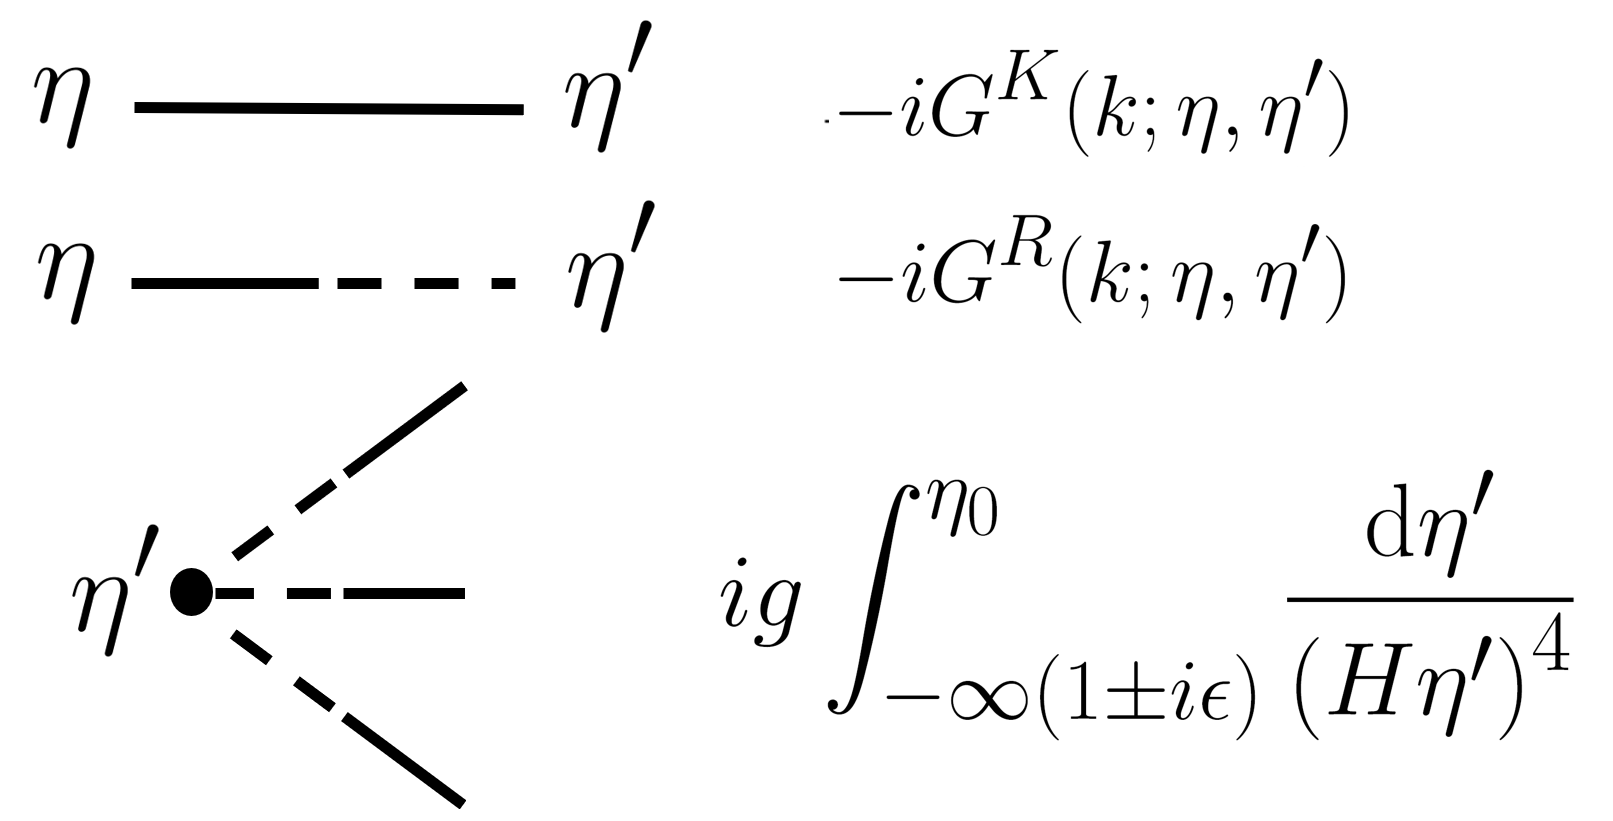
\includegraphics[width=0.5\textwidth]{figures/Rules.png}
\caption{Keldysh 基底での Feynman 則。}
\label{fig:rules}
\end{figure}

\subsectionlink{平坦時空での直観}\label{subsec:flatB}

原始宇宙論に移る前に、散逸のある Minkowski 時空で接触型三点関数の一般構造を考える。\Fig{fig:rules} の Feynman 則と \Eqs{eq:retardedM4dissip}、\eqref{eq:distribM4dissip} の伝播関数を用いる。\Eqs{eq:L13}、\eqref{eq:L23}、\eqref{eq:L33} のユニタリおよび非ユニタリな演算子をともに扱う。説明を明確にするため $\beta_2=\beta_4=0$ とするが、非零の場合へ拡張できる。また簡単のため $c_s=1$ とする。散逸とノイズがないときのユニタリな結果の回復は \App{app:unit} で詳しく述べる。

\paragraph{$\dot{\pi}^3$ 相互作用} まず次の相互作用を考える。

\begin{align}\label{eq:cubicdot}
\mathcal{L}_{\mathrm{int}} = -\frac{\alpha}{3!}\left(\dot{\pi}^3_+ - \dot{\pi}^3_-\right) = -\frac{\alpha}{2} \left(\dot{\pi}_r^2 \dot{\pi}_a + \frac{1}{12} \dot{\pi}_a^3\right).
\end{align}

前の負号は、$\alpha>0$ を仮定すると Lorentz 符号系から生じる。\footnote{\Eqs{eq:L13}、\eqref{eq:L23}、\eqref{eq:L33} の EFT 構成では、これは $(4\alpha_2-3\alpha_1)/f_\pi^6=-\alpha/2$ および $(\delta_4-\delta_6)/f_\pi^6=-\alpha/24$ に相当し、確かにユニタリな方向上にある。}ユニタリでシフト対称な場合、$\dot{\pi}^3$ と $(\partial_i\pi)^2\dot{\pi}$ は Minkowski 時空で接触型バイスペクトルを生じない。$t\rightarrow-t$ と $\pi\rightarrow-\pi$ の時間反転対称性によるもので、各図が個別に消えることも直接確認できる。散逸はこの対称性を自発的に破り、各図から非零のバイスペクトルが現れる。

\begin{figure}[tbp]
\centering
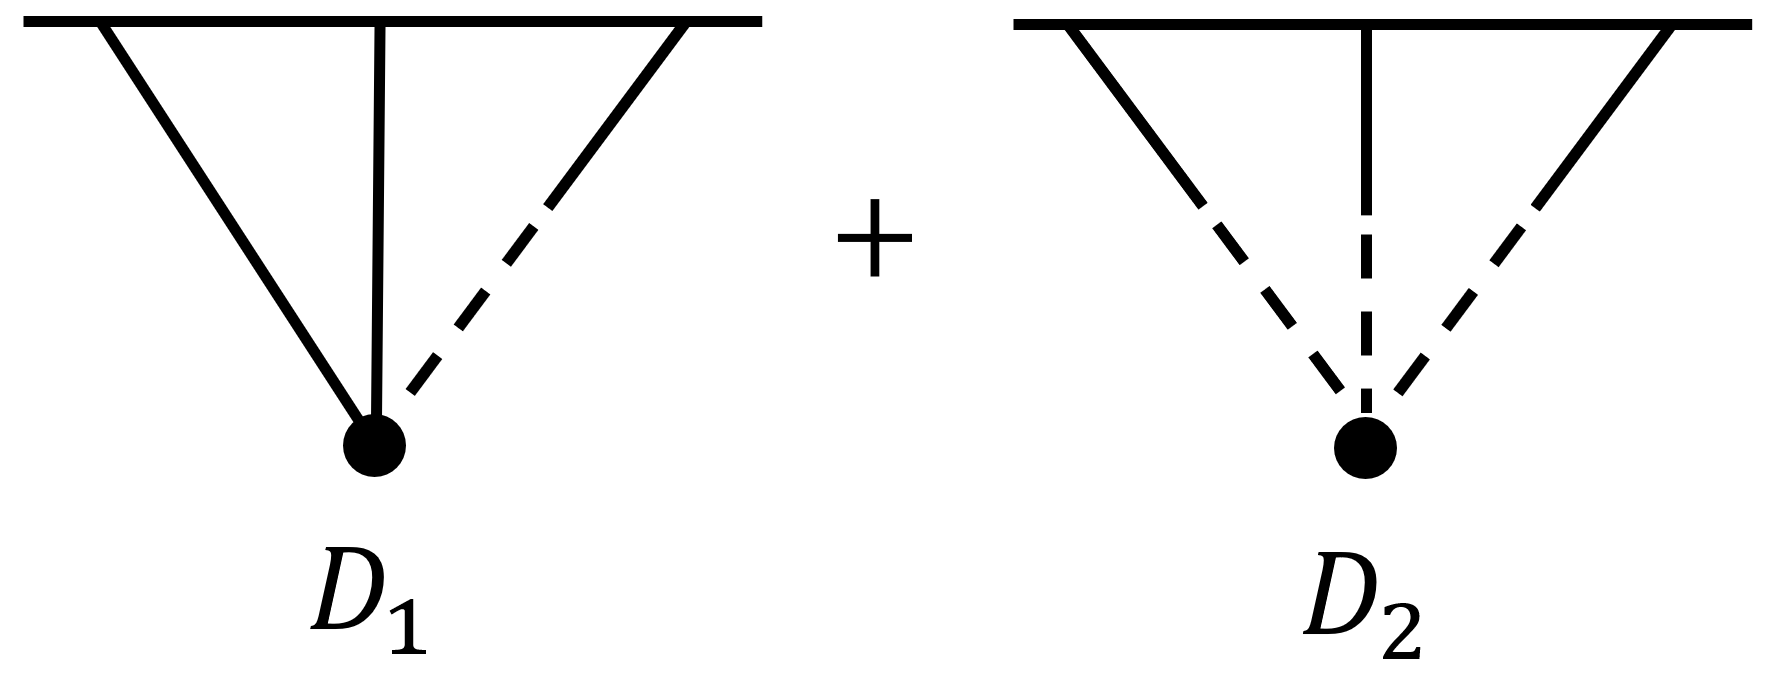
\includegraphics[width=0.5\textwidth]{figures/Btree.png}
\caption{\Eq{eq:cubicdot} の相互作用を計算する二つの図。左は $\dot{\pi}_r^2\dot{\pi}_a$ の頂点に対応し \Eqs{eq:D1dot} を与える。右は $\dot{\pi}_a^3$ の頂点に対応し \eqref{eq:D2dissip} を与える。}
\label{fig:Btree}
\end{figure}

バイスペクトルを次のように定義する。

\begin{align}\label{eq:bispecdef}
\langle \pi_{\bmk_1}  \pi_{\bmk_2}  \pi_{\bmk_3} \rangle \equiv (2\pi)^3 \delta(\bmk_1 + \bmk_2 + \bmk_3) B_\pi(k_1,k_2,k_3).
\end{align}

\Fig{fig:Btree} の二つの接触図を考え、その和が $B_\pi(k_1,k_2,k_3)=D^{\dot{\pi}^3}_1+D^{\dot{\pi}^3}_2$ となる。最初の図は次を与える。

\begin{align}\label{eq:D1dot}
D^{\dot{\pi}^3}_1 &=  \frac{\alpha}{2} \int_{-\infty(1\pm i \epsilon)}^{t_0} \dd t \left[\partial_t G^K(k_1; t_0,t)\right] \left[\partial_t G^K(k_2; t_0,t)\right] \left[\partial_tG^R(k_3; t_0,t)\right] + 5~\mathrm{perms}. 
\end{align}

\Eqs{eq:retardedM4dissip}、\eqref{eq:distribM4dissip} を \Eq{eq:D1dot} に代入し、六つの置換を足すと $D^{\dot{\pi}^3}_1=0$ となる。二つ目の図は $\pia$ 成分だけから成り、次の形をとる。

\begin{align}\label{eq:D2dissip}
D^{\dot{\pi}^3}_2 = \frac{\alpha}{24} \int_{-\infty(1\pm i \epsilon)}^{t_0} \dd t \left[\partial_t G^R(k_1; t_0,t) \right] \left[\partial_t G^R(k_2; t_0,t)\right] \left[ \partial_t G^R(k_3; t_0,t)\right] + 5~\mathrm{perms}.
\end{align}

同じ計算により、非零のバイスペクトルを得る。

\begin{align}\label{eq:D2resultdissip}
 B_\pi(k_1,k_2,k_3) &=  \frac{\alpha \gamma}{2} \frac{  \mathrm{Poly}_6\left(e_1^\gamma, e_2^\gamma,e_3^\gamma \right)}{ \mathrm{Sing}_\gamma} ,
\end{align}

ここで特異性の構造を次で定義した。

\begin{align}\label{eq:singdissip}
 \mathrm{Sing}_\gamma =& \left| E_1^{\gamma} + E_2^{\gamma} + E_3^{\gamma} + \frac{3}{2}i \gamma\right|^2 \left| -E_1^{\gamma} + E_2^{\gamma} + E_3^{\gamma} + \frac{3}{2}i \gamma\right|^2 \nonumber\\
 &\times \left| E_1^{\gamma} - E_2^{\gamma} + E_3^{\gamma} + \frac{3}{2}i \gamma\right|^2 \left| E_1^{\gamma} + E_2^{\gamma} - E_3^{\gamma} + \frac{3}{2}i \gamma\right|^2, 
\end{align}

$E_k^\gamma=\sqrt{c_s^2k^2-\gamma^2/4}$ を思い出そう。この特異性構造は非ユニタリなダイナミクスの特徴の大半を捉える。これは次の形の時間積分から生じる。

\begin{align}\label{eq:M4int}
\int_{-\infty(1\pm i \epsilon)}^{t_0} \dd t \ee^{ \pm i E_1^{\gamma} (t_0 - t) } \ee^{\pm i E_2^{\gamma} (t_0 - t) } \ee^{\pm i E_3^{\gamma} (t_0 - t) } \ee^{- \frac{3}{2}\gamma(t_0-t)}\,,
\end{align}

これは \Eqs{eq:retardedM4dissip}、\eqref{eq:distribM4dissip} の伝播関数の構造に由来する。物理的には環境が媒介する $3\leftrightarrow0$ および $2\leftrightarrow1$ 相互作用を表す。揺らぎは折り畳み特異性を生む一方、散逸は極を移動させ発散を正則化する。したがって特異点は物理的な平面上になく、全運動学的領域でバイスペクトルの摂動論的制御が保たれる。後述するように、この特異性構造は相互作用の細部に依存しない普遍的なものである。個々の相互作用の情報は、以下の基本対称多項式からなる $n$ 次多項式 $\mathrm{Poly}_n$ に記録される。

\begin{align}\label{eq:var}
e_1^\gamma = E_1^{\gamma} + E_2^{\gamma} + E_3^{\gamma}, \quad e_2^\gamma = E_1^{\gamma} E_2^{\gamma} + E_2^{\gamma}  E_3^{\gamma} + E_1^{\gamma} E_3^{\gamma} \quad  e_3^\gamma = E_1^{\gamma} E_2^{\gamma} E_3^{\gamma}.
\end{align}

この場合の $\mathrm{Poly}_6$ の明示形は次のとおりである。

\begin{align}
\mathrm{Poly}_6\left(e_1^\gamma, e_2^\gamma,e_3^\gamma \right) &= 243\gamma^6 - 792 \gamma^4 e_2^\gamma + 396 \gamma^4 \left(e_1^\gamma\right)^2 + 576 \gamma^2 \left(e_2^\gamma\right)^2 -1088 \gamma^2 e_2^\gamma\left(e_1^\gamma\right)^2 \nonumber \\
&+272 \gamma^2 \left(e_1^\gamma\right)^4 + 1024 \gamma^2e_1^\gamma e_3^\gamma + 512 \left(e_1^\gamma\right)^2 \left(e_2^\gamma\right)^2 - 384 \left(e_1^\gamma\right)^4 e_2^\gamma \\
&-1024 e_1^\gamma e_2^\gamma e_3^\gamma + 64 \left(e_1^\gamma\right)^6 + 512 e_3^\gamma \left(e_1^\gamma\right)^3 + 768 \left(e_3^\gamma\right)^2. \nonumber
\end{align}

\begin{figure}[tbp]
\centering
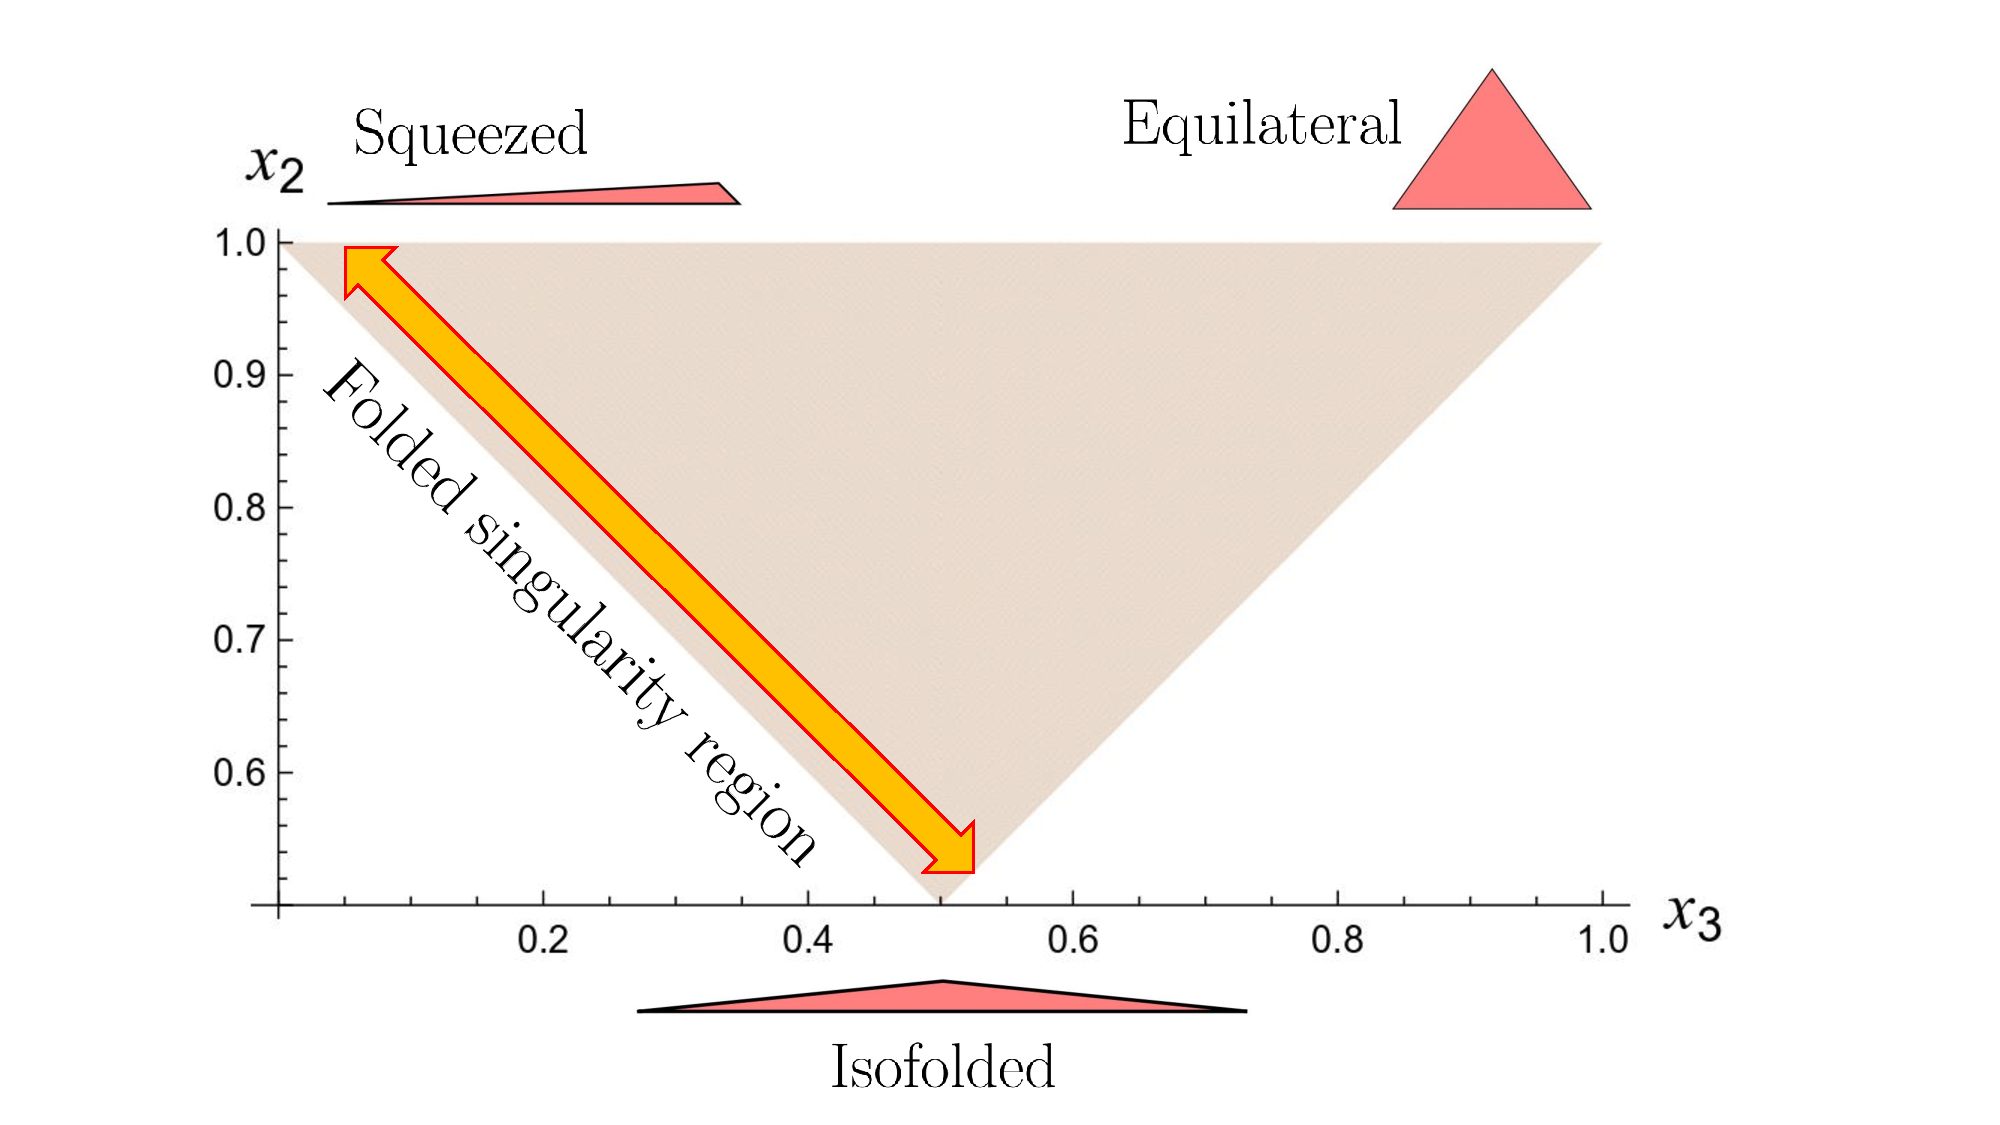
\includegraphics[width=0.7\textwidth]{figures/triangles_fin.pdf}
\caption{運動量保存 $\delta(\bmk_1+\bmk_2+\bmk_3)$ を満たす三角形の形状。$x_2\equiv k_2/k_1$、$x_3\equiv k_3/k_1$ とし、閉じた三角形を作る条件 $x_3<x_2<1$、$x_2+x_3>1$ を満たす。特に関心があるのは $x_2+x_3\simeq1$ の折り畳み領域で、スクイーズ配置と等脚折り畳み配置をつなぐ。\Eq{eq:singdissip} の特異性構造はこの領域付近でピークをもち、散逸的ダイナミクスの明瞭な兆候を与える。}
\label{fig:triangles}
\end{figure}

この相互作用が生むバイスペクトルの形状を考えよう。\Eq{eq:bispecdef} の運動量保存 $\delta(\bmk_1+\bmk_2+\bmk_3)$ により、運動量は閉じた三角形をなす必要がある。インフレーション模型ごとに信号が最大になる三角形配置が異なるため（例えば \cite{Babich:2004gb,Chen:2006nt}）、次の形状関数が有用である。

\begin{align}\label{eq:shaperef}
S(x_2,x_3) \equiv (x_2 x_3)^2 \frac{B(k_1, x_2 k_1, x_3 k_1)}{B(k_1,k_1,k_1)}
\end{align}

これは原始非ガウス性を生む機構を調べる手掛かりとなる。$x_2\equiv k_2/k_1$ と $x_3\equiv k_3/k_1$ は三角形の形を指定し、運動量保存 $\delta(\bmk_1+\bmk_2+\bmk_3)$ から $\max(x_3,1-x_3)\leq x_2\leq1$ に制限される。\Fig{fig:triangles} に本論文で主に関心のある配置を示す。\Eq{eq:singdissip} の $\mathrm{Sing}_\gamma$ は散逸係数 $\gamma$ の大きさによって二通りに振る舞う。散逸が強い場合は \Eq{eq:singdissip} の $\frac32i\gamma$ が常に寄与を支配し、信号は $x_2\simeq x_3\simeq1$ の正三角形配置で最大となる（\Fig{fig:shapeMink} 右）。散逸が小さい場合は $x_2+x_3\simeq1$ の折り畳み領域で $\mathrm{Sing}_\gamma$ が小さくなり、$x_2\simeq x_3\simeq1/2$ の等脚折り畳み配置の近くで主にピークを示す（\Fig{fig:shapeMink} 左）。

\begin{figure}[tbp]
\centering 
\makebox[\textwidth][c]{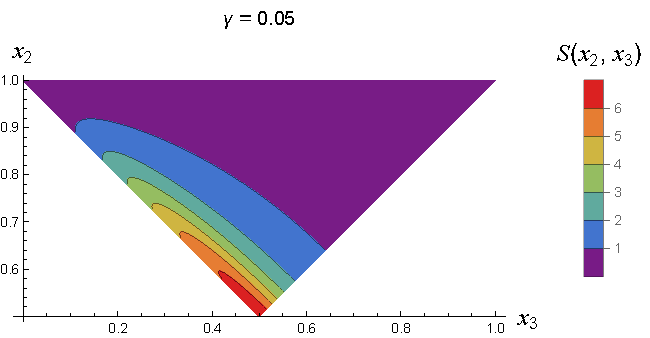
\includegraphics[width=.5\textwidth]{figures/Folded.pdf}
    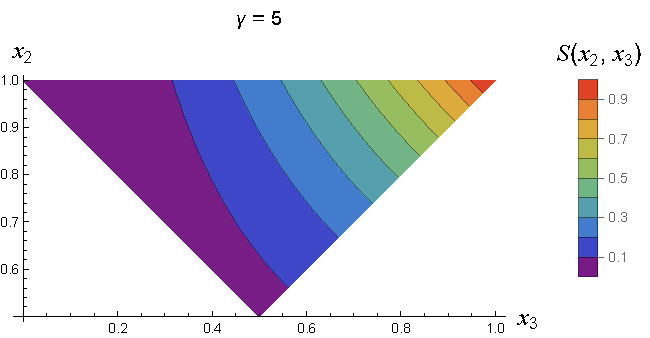
\includegraphics[width=.5\textwidth]{figures/Equil.pdf}}
\caption{\label{fig:shapeMink}\Eq{eq:D2resultdissip} の Minkowski 時空の $\dot{\pi}_a^3$ が生む接触型バイスペクトルの形状関数。左：散逸が小さいと、\Eq{eq:singdissip} の $\mathrm{Sing}_\gamma$ が $x_2+x_3\simeq1$ の折り畳み領域で小さくなり、バイスペクトルが増強される。右：散逸が大きいと、散逸による虚数項が $\mathrm{Sing}_\gamma$ を支配し、折り畳み領域での増強は見られない。}
\end{figure}

同様の特異性は、主として非 Bunch--Davies 初期状態の宇宙論で知られている \cite{Holman:2007na,Chen:2006nt,Meerburg:2009ys,Agullo:2010ws,Ashoorioon:2010xg,Agarwal:2012mq,Ashoorioon:2013eia,Albrecht:2014aga,Green:2020whw}。ここでは散逸的環境があるため、$\gamma\neq0$ なら $\mathrm{Sing}_\gamma\neq0$ となり、折り畳み特異性が正則化される点が異なる。\Fig{fig:foldedMink} 右上のパネルは、$x_2+x_3\simeq1$ に近づく際の形状関数のピークを示す。特異性が解消されるので、すべての配置にわたり摂動論的制御を保てる。散逸相互作用に対処するための人工的なカットオフは不要である。

\begin{figure}[tbp]
\begin{minipage}{6in}
    \centering
    \raisebox{-0.5\height}{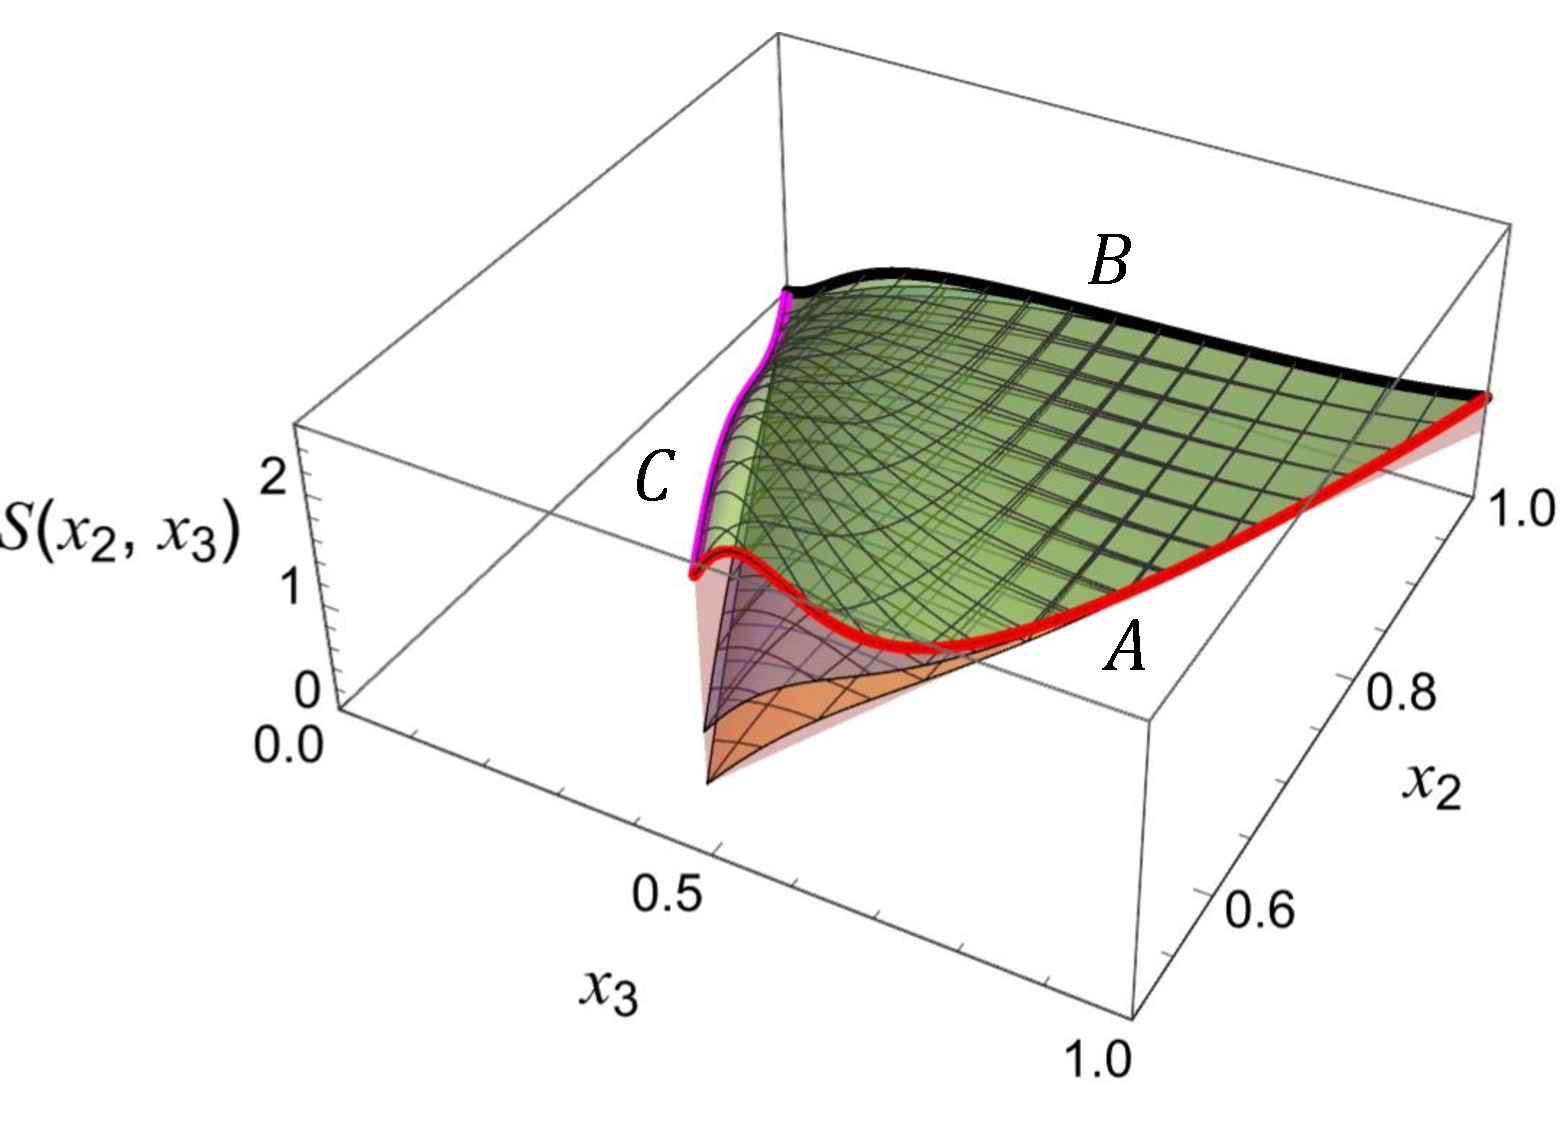
\includegraphics[width=.45\textwidth]{figures/3d.pdf}}
    \raisebox{-0.5\height}{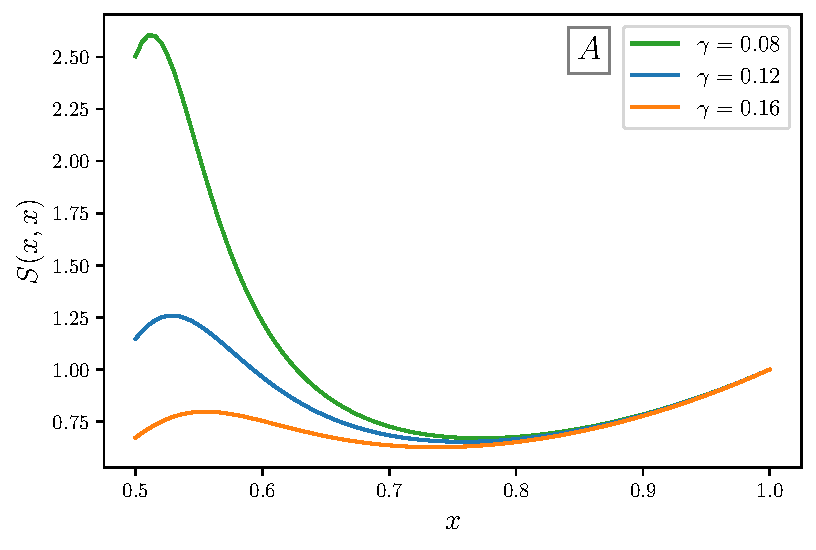
\includegraphics[width=.45\textwidth]{figures/2dcutA.pdf}}
        \centering
    \raisebox{-0.5\height}{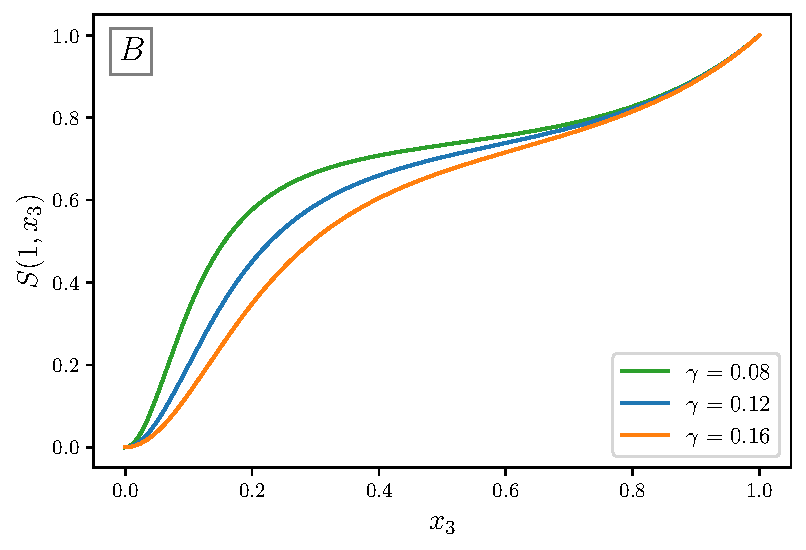
\includegraphics[width=.45\textwidth]{figures/2dcutB.pdf}}
    \raisebox{-0.5\height}{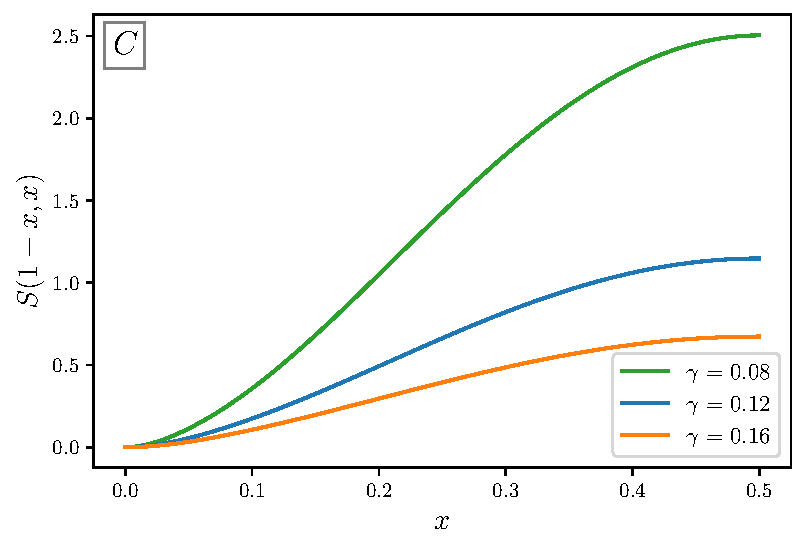
\includegraphics[width=.45\textwidth]{figures/2dcutC.pdf}}
\end{minipage}
\caption{\label{fig:foldedMink}左上は、\Eq{eq:D2resultdissip} の Minkowski 時空における $\dot{\pi}_a^3$ が生む接触型バイスペクトルの三次元形状関数を、$\gamma=0.08,0.12,0.16$ について示す。$\gamma$ が減るにつれ、正三角形配置から折り畳み配置へピークが移る。右上は赤線 $x_2=x_3=x$ に沿う二次元断面。特異性が解消され、任意の三角形配置と散逸パラメータ $\gamma$ に対してバイスペクトルがよく定義される。左下は黒線 $x_2=1$ に沿う二次元断面。整合関係により $x_3\ll1$ のスクイーズ極限で信号は消える。右下は紫線 $x_2=1-x_3$ に沿う二次元断面。同じくスクイーズ極限で整合関係が見られる。}
\end{figure}

\paragraph{他の相互作用} 他の相互作用も同じ構造に従う。表 \ref{tab:cubicdissip} には \Eqs{eq:L13}、\eqref{eq:L23}、\eqref{eq:L33} の三次相互作用が生む非零の接触型バイスペクトルをまとめる。\footnote{$(\partial_i\pir)^2\dot{\pi}_a$ と $\dot{\pi}_r\partial_i\pir\partial^i\pia$ はそれぞれ \Eq{eq:gen} 型の非零の寄与を与えるが、\Eq{eq:L13} に現れる $\alpha_1(\partial_i\pir)^2\dot{\pi}_a+2\alpha_1\dot{\pi}_r\partial_i\pir\partial^i\pia$ の組合せでは、二つの寄与が完全に相殺し、バイスペクトルはゼロになる。}一般形は次のとおりである。
\begin{tcolorbox}[
enhanced,
breakable,
skin first=enhanced,
skin middle=enhanced,
skin last=enhanced,
before upper={\parindent15pt},
]{}

\paragraph{Minkowski 時空の散逸的バイスペクトル}

\begin{align}\label{eq:gen}
    B_\pi(k_1,k_2,k_3) =f(\mathrm{EFT}) \frac{  \mathrm{Poly}_n\left(e_1^\gamma, e_2^\gamma,e_3^\gamma \right)}{ \mathrm{Sing}_\gamma} 
\end{align}

ここで $f(\mathrm{EFT})$ は EFT 係数の有理関数であり、空間微分を含む相互作用では運動学変数にも依存しうる。$\mathrm{Poly}_n$ は \Eq{eq:var} の変数の多項式、$\mathrm{Sing}_\gamma$ は \Eq{eq:singdissip} の特異性構造である。

\end{tcolorbox}

\Eq{eq:M4int} 型の積分に由来するこの構造の単純さは、局所的な散逸ダイナミクスに対する bootstrap 手法の将来の発展を示唆する。また、$\mathrm{Sing}_\gamma$ が環境に媒介される $3\leftrightarrow0$ と $2\leftrightarrow1$ 相互作用の振幅を制御するという解釈によって、物理がよく捉えられていることも示唆する。

\begin{table}
\centering
\begin{tabular}{cc}
     $\left(4 \gamma_2 -\frac{\gamma}{2} \right)  \dot{\pi}^2_{r} \pia$ & $B_\pi =  -  \frac{3\left(8 \gamma_2 - \gamma  \right)}{2\gamma^2} \frac{\beta_1^2}{f_\pi^6 } \frac{  \mathrm{Poly}_4\left(e_1^\gamma, e_2^\gamma,e_3^\gamma \right)}{ \mathrm{Sing}_\gamma} \Bigg.$ \\
    $\frac{\gamma}{2} 	\left(\partial_i \pir \right)^2 \pia $ & $B_\pi = - \frac{8\gamma}{\gamma^2} \frac{\beta_1^2}{f_\pi^6} \frac{K^2}{ k_1^2 k_2^2 k_3^2} \Bigg.$\\
    $i\beta_3 \partial_i \pir  \partial^i \pia \pia$ & $B_\pi = \frac{\beta_3}{16} \frac{\beta_1}{f_\pi^6}  \frac{K^2}{k_1^2 k_2^2 k_3^2} \frac{  \mathrm{Poly}_8\left(e_1^\gamma, e_2^\gamma,e_3^\gamma \right)}{ \mathrm{Sing}_\gamma}  \Bigg.$ \\
    $2 i\left(\beta_4 + \beta_6 - \beta_8 \right) \dot{\pi}_{r} \dot{\pi}_a^2$ & $B_\pi =   \frac{\beta_4 + \beta_6 - \beta_8}{8\gamma}  \frac{\beta_1}{f_\pi^6} \frac{  \mathrm{Poly}_6\left(e_1^\gamma, e_2^\gamma,e_3^\gamma \right)}{ \mathrm{Sing}_\gamma}  \Bigg.$  \\
    $- 2i \left[\beta_4   \partial_i \pir  \partial^i \pia \dot{\pi}_{a} +  \beta_5   \dot{\pi}_{r}  \pia^2 + \beta_6   \dot{\pi}_{r} (\partial_i \pia)^2\right]$ & $B_\pi = \frac{3\left[\left(2\beta_6 - \beta_4\right)K^2 - \beta_5\right] }{\gamma} \frac{\beta_1}{f_\pi^6}  \frac{  \mathrm{Poly}_4\left(e_1^\gamma, e_2^\gamma,e_3^\gamma \right)}{ \mathrm{Sing}_\gamma}  \Bigg.$  \\ 
    $\delta_1 \pi^3_a + \delta_2 (\partial_i \pia)^2\pia$ & $B_\pi = - \frac{3}{4} \frac{\delta_1 - \delta_2 K^2}{f_\pi^6} \frac{  \mathrm{Poly}_4\left(e_1^\gamma, e_2^\gamma,e_3^\gamma \right)}{ \mathrm{Sing}_\gamma} \Bigg.$\\
    $\left(\delta_5-\delta_2 \right)\dot{\pi}_a^2 \pia $ & $B_\pi = \frac{1}{32} \frac{\delta_2-\delta_5}{f_\pi^6} \frac{  \mathrm{Poly}_6\left(e_1^\gamma, e_2^\gamma,e_3^\gamma \right)}{ \mathrm{Sing}_\gamma} \Bigg.$\\
    $\left(\delta_4-\delta_6 \right)\dot{\pi}_a^3$ & $B_\pi = \frac{3\gamma}{16} \frac{\delta_6-\delta_4}{f_\pi^6} \frac{  \mathrm{Poly}_6\left(e_1^\gamma, e_2^\gamma,e_3^\gamma \right)}{ \mathrm{Sing}_\gamma} \Bigg.$\\
\end{tabular}
\caption{\Eqs{eq:L13}、\eqref{eq:L23}、\eqref{eq:L33} の三次相互作用が接触型バイスペクトルへ与える非零の寄与。$\mathrm{Sing}_\gamma$ は \Eq{eq:singdissip} に示し、$K^2\equiv\bmk_1\cdot\bmk_2+\bmk_1\cdot\bmk_3+\bmk_2\cdot\bmk_3$ と定義した。$\mathrm{Poly}_n$ は \Eq{eq:var} の変数の多項式である。読みやすさのためその詳細は省略した。}
\label{tab:cubicdissip}
\end{table}

\subsectionlink{散逸とノイズによる非ガウス性}\label{subsec:bispecdS}

散逸ダイナミクスがユニタリな場合とどう異なるかについて見通しが得られたので、これらの手法を原始宇宙論に適用する。空間的に平坦なゲージで曲率摂動が $\zeta=-H\pi/f_\pi^2$ と定義されることを用いると、原始バイスペクトルは次のとおりである。

\begin{align}
    \langle \zeta_{\bmk_1}  \zeta_{\bmk_2}  \zeta_{\bmk_3} \rangle  = - \frac{H^3}{f_\pi^6}	\langle \pi_{\bmk_1}  \pi_{\bmk_2}  \pi_{\bmk_3} \rangle \equiv (2\pi)^3 \delta(\bmk_1 + \bmk_2 + \bmk_3) B(k_1,k_2,k_3).
\end{align}

非ガウス的信号を特徴付ける量は、以下の信号振幅と形状関数である。

\begin{align}
    f_{\mathrm{NL}}(k_1,k_2,k_3) \equiv \frac{5}{6} \frac{B(k_1,k_2,k_3)}{P(k_1) P(k_2) +  P(k_1) P(k_3)  + P(k_2) P(k_3) }\,,
\end{align}

振幅については後で特定の配置について論じる。形状関数は \Eq{eq:shaperef} で定義済みだが、明確にするため再掲する。

\begin{align}
    S(x_2,x_3) \equiv (x_2 x_3)^2 \frac{B(k_1, x_2 k_1, x_3 k_1)}{B(k_1,k_1,k_1)}\,.
\end{align}

$x_2\equiv k_2/k_1$、$x_3\equiv k_3/k_1$ は $\max(x_3,1-x_3)\leq x_2\leq1$ に制限される。\Sec{subsec:flatB} の平坦時空と同じ手順で接触型バイスペクトルを評価できる。積分の一般的な構造は次のとおりである。

\begin{align}\label{eq:Bexpref}
    &B(k_1,k_2,k_3) = (-i)^{n_K + n_R + 1}\frac{H^3}{f_\pi^6} \frac{g}{H^{4-n_d}} \int_{-\infty(1 \pm i \epsilon)}^{0^-} \frac{\dd \eta}{\eta^{4-n_d}} \nonumber \\
    &\qquad \widehat{\mathcal{D}}(\{\bmk_i\}, \partial_\eta)\left[ G^{K/R}(k_1, 0, \eta) G^{K/R}(k_2, 0, \eta) G^R(k_3, 0, \eta) + 5~\mathrm{perms}. \right]
\end{align}

ここで $n_K$ は Keldysh 伝播関数、$n_R$ は遅延伝播関数、$n_d$ は空間および時間微分の個数を数える。$\widehat{\mathcal{D}}(\{\bmk_i\},\partial_\eta)$ は、伝播関数に作用する $n_d$ 次の空間・時間微分を模式的に表す微分演算子である。\Eq{eq:norm} から $\pia$ に少なくとも線形であるため、$G^R$ は必ず一つ以上含まれる。bulk-to-boundary 伝播関数は次で与えられる。

\begin{align}\label{eq:GRB2b}
    G^R(k, 0, \eta) = -\frac{H^2}{2k^3}  z^{3} \left(\frac{z}{2} \right)^{ - \nu_\gamma}\Gamma(z) J_{\nu_\gamma}(z)
\end{align}

また、

\begin{align}
    G^K(k, 0,\eta) &= - i\frac{\pi}{4k^3} \beta_1 \left(2 z \right)^{\nu_\gamma} \Gamma(\nu_\gamma) \left[ Y_{\nu_\gamma}(z)A^{(1)}_{\nu_\gamma}(z)- J_{\nu_\gamma}(z)B^{(1)}_{\nu_\gamma}(z)\right]\,,
\end{align}

ここでは $z=-k\eta$、$\nu_\gamma=\frac32+\frac{\gamma}{2H}$ を用い、$A^{(1)}_{\nu_\gamma}(z)$、$B^{(1)}_{\nu_\gamma}(z)$ はそれぞれ \Eqs{eq:Fbetaref}、\eqref{eq:Gbetaref} で定義した。時間微分も有用である。

\begin{align}
    \partial_\eta G^R(k, 0,\eta) = \frac{H^2}{2k^2} z^2 \left(\frac{z}{2} \right)^{-\nu_\gamma} \Gamma (\nu_\gamma) \left[ z J_{\nu_\gamma -1}(z)- (2 \nu_\gamma-3) J_{\nu_\gamma}(z)\right]
\end{align}

さらに、

\begin{align}
    \partial_\eta G^K(k, 0,\eta)&= i\frac{\pi}{4k^2}\beta_1\left(2 z \right)^{\nu_\gamma-1} \Gamma(\nu_\gamma)  \bigg\{\left[-z Y_{\nu_\gamma+1}(z)+2\nu_\gamma Y_{\nu_\gamma}(z) + z Y_{\nu_\gamma-1}(z)\right]A^{(1)}_{\nu_\gamma}(z) \nonumber \\
    & \left[-z J_{\nu_\gamma+1}(z)+2\nu_\gamma J_{\nu_\gamma}(z) + z J_{\nu_\gamma-1}(z)\right]B^{(1)}_{\nu_\gamma}(z)\bigg\}.
\end{align}

これらの伝播関数の式を代入して \Eq{eq:Bexpref} の時間積分を評価する。一般の場合に解析的な実行は難しいため、以下では主に数値積分を使い、特定の領域だけで解析的な結果を導く。

\subsubsection*{数値結果}

\Eqs{eq:L13}、\eqref{eq:L23}、\eqref{eq:L33} の三次演算子が生む接触型バイスペクトルの主な現象論的帰結をまとめる。網羅的な調査は将来に譲り、この種類の模型に予想される信号の主要な特徴に焦点を当てる。解析に用いた \textit{Mathematica} コードは要請に応じて提供できる。

\Eqs{eq:L13}、\eqref{eq:L23}、\eqref{eq:L33} の十六個の三次演算子の多くは似た特徴を生む。そのため、以下の基準で選んだ一部だけの結果を示す。
\begin{itemize}
\item \Eq{eq:L13} の $\mathcal{L}_1$ から、通常のインフレーション EFT に戻るユニタリ極限でも現れる $\dot{\pi}_r^2\dot{\pi}_a$ と $(\partial_i\pir)^2\dot{\pi}_a$ を選ぶ。伝播関数の構造の変化により、散逸がこれらの特徴をどう変えるか示す。
\item \Eq{eq:L13} の $\mathcal{L}_1$ から、非線形に実現された boost によって二次の散逸項 $\dot{\pi}_r\pia$ と結び付く $\dot{\pi}_r^2\pia$、$(\partial_i\pir)^2\pia$ も扱う。\cite{LopezNacir:2011kk} は主に強い散逸の場合を論じたが、ここでは弱い散逸の場合の結果で補う。
\item \Eq{eq:L23} の $\mathcal{L}_2$ から $\partial_i\pir\partial^i\pia\pia$ と $\dot{\pi}_r\pia^2$ を選ぶ。前者は、一次の次数では全微分 $\dot{\pi}_a\pia$ となるノイズ項 $(P^\mu\partial_\mu\pia)\pia$ に boost を非線形に実現することで生じる。後者は、\cite{Creminelli:2023aly} が初めて指摘し \Sec{sec:matching} でも論じる、$\gamma/H$ に対する $f_{\mathrm{NL}}^{\mathrm{eq}}$ の興味深い特徴を示す。
\item \Eq{eq:L33} の $\mathcal{L}_3$ からは、通常のインフレーション EFT を回復するユニタリ極限にも現れる $\dot{\pi}_a^3$ を選ぶ。微分を含まないため異なる振る舞いが懸念される $\pia^3$ も扱うが、ユニタリな場合と異なる伝播関数によって、これも概ね他の相互作用と同様の特徴を示す。
\end{itemize}
$\pir^{\prime2}\pia$、$(\partial_i\pir)^2\pia$、$\pir'\pia^2$、$\pia^3$ は、\Sec{sec:matching} で論じる \cite{Creminelli:2023aly} の UV 完成との対応にも現れる四つの三次演算子である。これらが生む接触型バイスペクトルの形状を \Figs{fig:shapes_high}、\ref{fig:shapes_low} に示す。他の演算子も本質的には同様の傾向に従う。平坦時空の場合と同様、強い散逸 $\gamma\gg H$ と弱い散逸 $\gamma\ll H$ では振る舞いが異なる。前者は \cite{LopezNacir:2011kk} がすでに指摘したように正三角形配置でピークを示し、後者は折り畳み領域の近くで極値をとる。

\begin{figure}[tbp]
\sidesubfloat[]{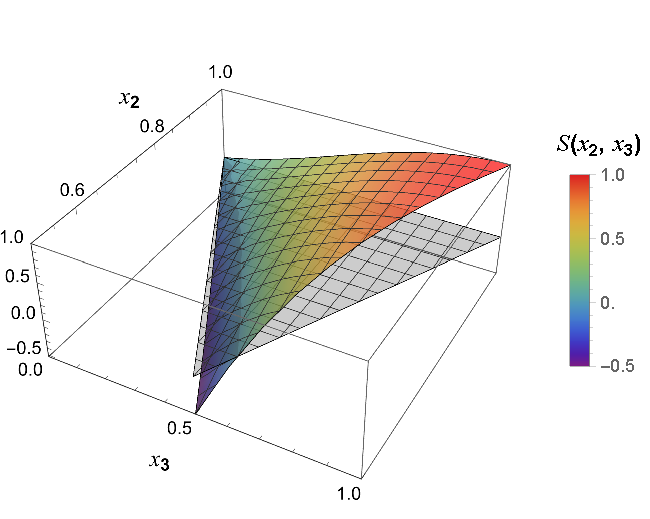
\includegraphics[width=0.4\textwidth]{figures/Shape1_high.pdf}\label{fig:c}}
\hfil
\sidesubfloat[]{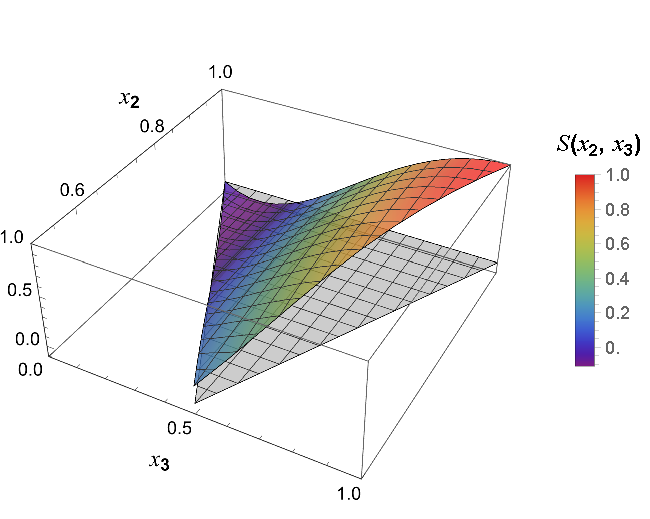
\includegraphics[width=0.4\textwidth]{figures/Shape2_high.pdf}\label{fig:d}}

\medskip
\sidesubfloat[]{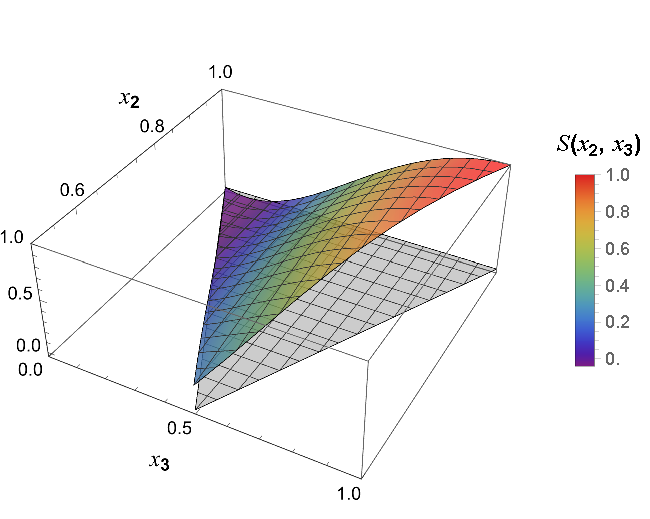
\includegraphics[width=0.4\textwidth]{figures/Shape8_high.pdf}\label{fig:e}}
\hfil
\sidesubfloat[]{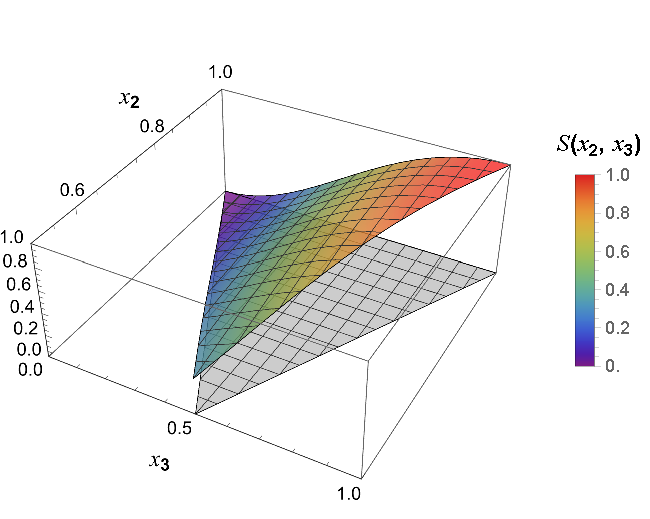
\includegraphics[width=0.4\textwidth]{figures/Shape4_high.pdf}\label{fig:f}}
\caption{強い散逸 $\gamma=5H$ の場合のバイスペクトル形状。この領域では $x_2=x_3=1$ の正三角形配置で信号が最大になる。$x_3\ll x_2=1$ のスクイーズ極限でも整合関係を満たす。\textbf{a：}$(\partial_i\pir)^2\pia$、\textbf{b：}$\dot{\pi}_r^2\pia$、\textbf{c：}$\dot{\pi}_r\pia^2$、\textbf{d：}$\pia^3$。}
    \label{fig:shapes_high}
    \end{figure}

\begin{figure}[tbp]
    \centering
\sidesubfloat[]{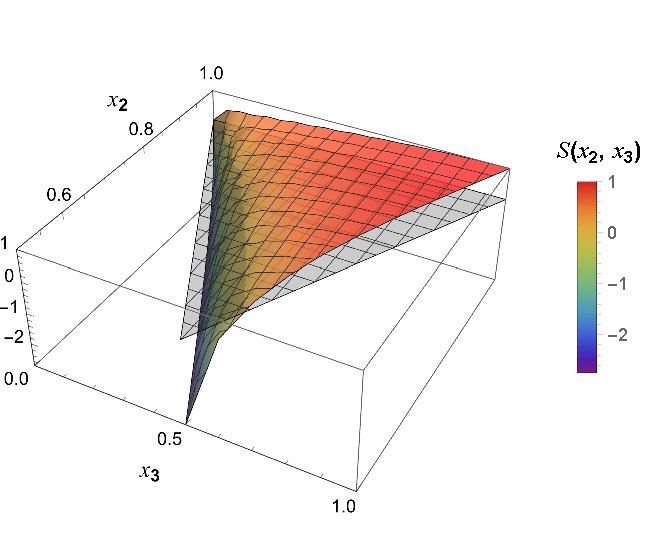
\includegraphics[width=0.4\textwidth]{figures/Shape1_low.pdf}\label{fig:cbis}}
\hfil
\sidesubfloat[]{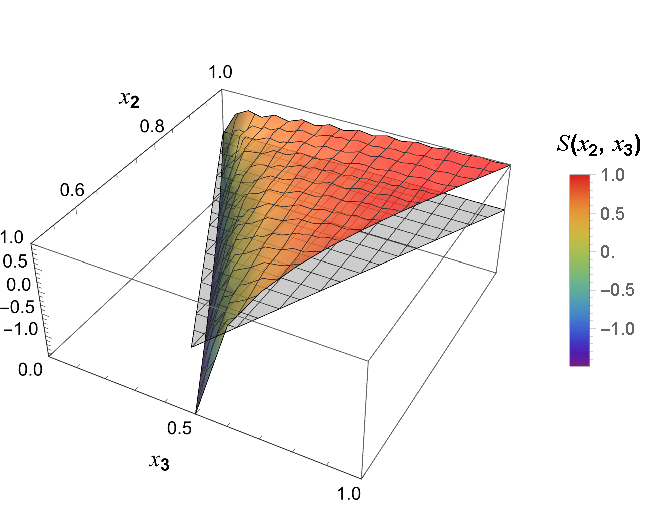
\includegraphics[width=0.4\textwidth]{figures/Shape2_low.pdf}\label{fig:dbis}}

\medskip
\sidesubfloat[]{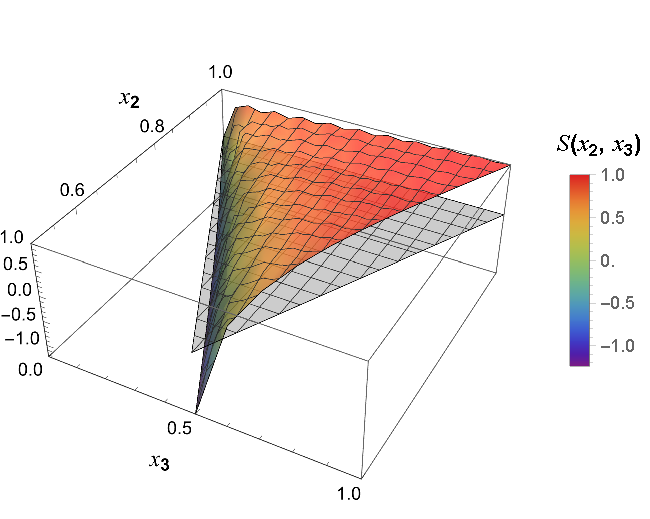
\includegraphics[width=0.4\textwidth]{figures/Shape8_low.pdf}\label{fig:ebis}}
\hfil
\sidesubfloat[]{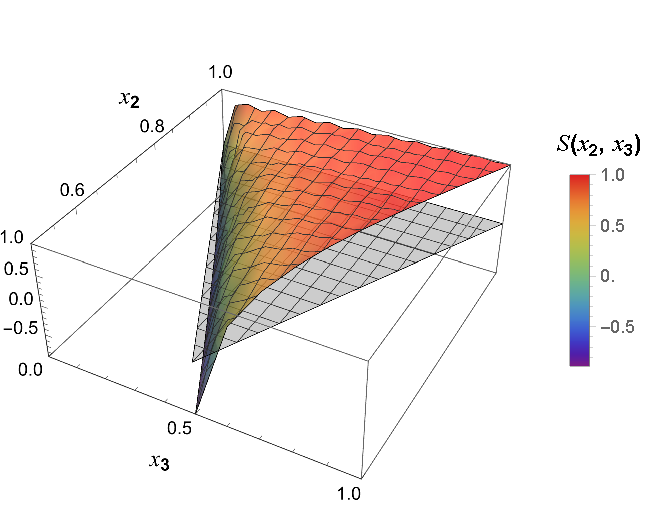
\includegraphics[width=0.4\textwidth]{figures/Shape4_low.pdf}\label{fig:fbis}}
\caption{弱い散逸 $\gamma=0.001H$ の場合のバイスペクトル形状。信号は $x_2+x_3=1$ の折り畳み配置付近で最大となる。$x_3\ll x_2=1$ のスクイーズ極限では整合関係が引き続き成り立つ。微小な振動は有限区間の数値積分による人工的なものである。\textbf{a：}$(\partial_i\pir)^2\pia$、\textbf{b：}$\dot{\pi}_r^2\pia$、\textbf{c：}$\dot{\pi}_r\pia^2$、\textbf{d：}$\pia^3$。}
    \label{fig:shapes_low}
    \end{figure}

開放ダイナミクスを示すこの特徴は、非 Bunch--Davies 初期状態 \cite{Holman:2007na,Chen:2006nt,Meerburg:2009ys,Agullo:2010ws,Ashoorioon:2010xg,Agarwal:2012mq,Ashoorioon:2013eia,Albrecht:2014aga,Green:2020whw} のように折り畳み三角形で信号を生む他の模型と縮退して見えるかもしれない。しかし決定的な違いがある。数値計算で見られ、以下の解析でも確認されるのは、散逸がピークを滑らかにして三角形配置の境界から移動させ、発散を正則化することである。したがって、物理的な任意の配置でバイスペクトルは有限になる。特に \Fig{fig:squeezed} の $k_1\simeq k_2\gg k_3$ のスクイーズ極限で発散しない。小さな $\gamma/H$ では正則化された折り畳み特異性に由来する中間的なピークが現れうるが、理論の対称性により整合関係 \cite{Maldacena:2002vr,Creminelli:2004yq,Cheung:2007sv,Creminelli:2012ed,Hinterbichler:2012nm,Assassi:2012zq,Pajer:2017hmb,Avis:2019eav} は成り立ち、スクイーズ極限でゼロへ向かう。$\pia^3$ のように微分を含まない演算子も、素朴な予想に反してこの傾向に従う。自由理論と比べて伝播関数が変化し、例えば赤外での収束が保証されるためである。

\begin{figure}[tbp]
\centering
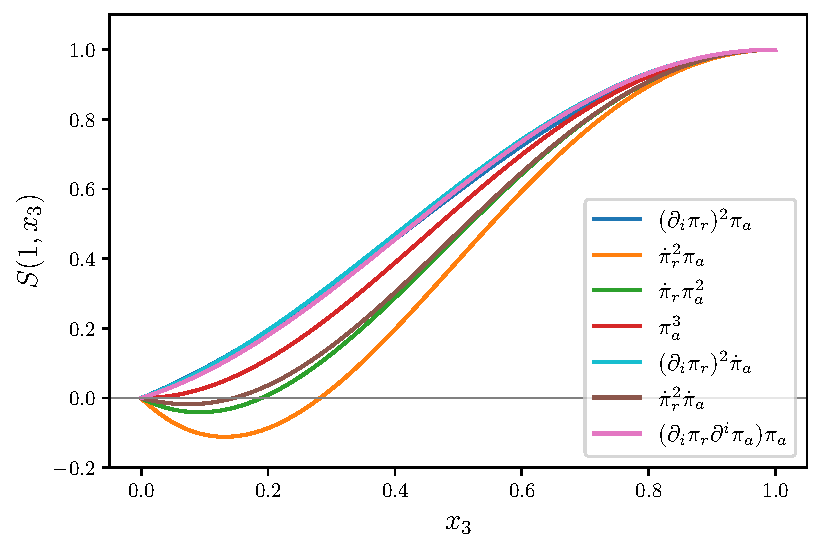
\includegraphics[width=0.6\textwidth]{figures/2dcut_dS_high.pdf}
\caption{強い散逸 $\gamma=5H$ における、接触型バイスペクトルのさまざまな寄与について、$x_2=1$ に沿った形状関数。整合関係により $x_3\ll1$ のスクイーズ極限で信号はゼロになる。}
\label{fig:squeezed}
\end{figure}

正三角形配置における振幅は次の量で特徴付けられる。

\begin{align}
    f_{\mathrm{NL}}^{\mathrm{eq}} \equiv \frac{10}{9} \frac{k^6}{(2\pi)^4}\frac{B(k,k,k)}{\Delta_\zeta^4}.
\end{align}

\Fig{fig:fnleq} では、上で扱った演算子について、$B(k,k,k)$ の数値積分で得た $f_{\mathrm{NL}}^{\mathrm{eq}}$ の $\gamma/H$ 依存性を示す。\cite{Planck:2019kim} の観測制約 $f_{\mathrm{NL}}^{\mathrm{eq}}=26\pm47$ を用い、強い散逸領域の EFT パラメータに制限を課せる。例えば $(\partial_i\pir)^2\pia$ の寄与を数値的に当てはめると $f_{\mathrm{NL}}^{\mathrm{eq}}\simeq-\gamma/(4H)$ となり、\cite{LopezNacir:2011kk,Creminelli:2023aly} および \Sec{subsec:energy} の発見的見積もりと一致する。素朴には $68\%$ 信頼水準で $\gamma/H<80$ を意味する。ただし、異なる三次演算子の寄与が累積し、互いに分離できないため、この制限は現実的な推定というより原理的可能性の実証である。それでも、この種類の模型をデータと比較する方法を示している。将来の SPHEREX \cite{SPHEREx:2014bgr} や MegaMapper \cite{Cabass:2022epm,Braganca:2023pcp} などの大規模構造観測は制約を強めうる。弱い散逸領域でも、次の量について同種の解析を考えられる。

\begin{align}
    f_{\mathrm{NL}}^{\mathrm{folded}} \equiv \frac{5}{24} \frac{k^6}{(2\pi)^4} \frac{B(k,k/2,k/2)}{\Delta_\zeta^2(k/2)[4\Delta_\zeta^2(k/2) + \Delta_\zeta^2(k) ]},
\end{align}

例えば CMB-BEST パイプライン \cite{PhysRevD.108.063504} を用いることができる。この解析は今後の課題とする。

\begin{figure}[tbp]
    \begin{minipage}{6in}
    \centering
    \raisebox{-0.5\height}{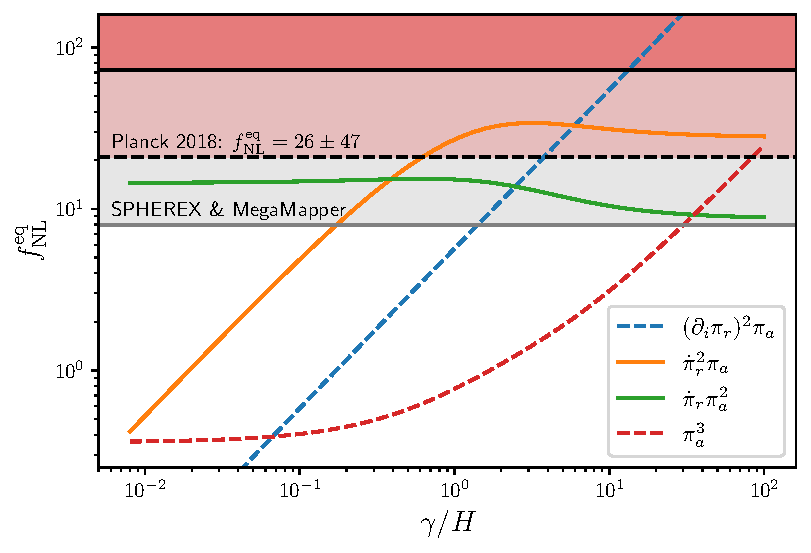
\includegraphics[width=.48\textwidth]{figures/fNL.pdf}}
    \raisebox{-0.5\height}{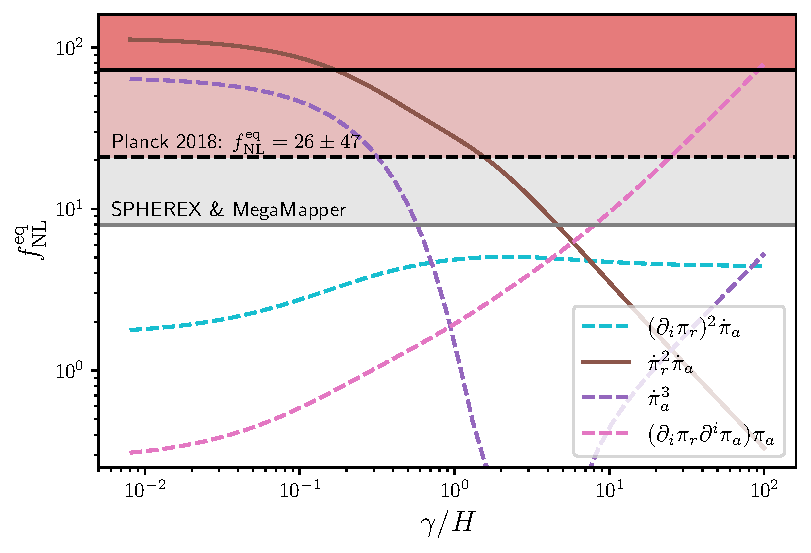
\includegraphics[width=.48\textwidth]{figures/fNLb.pdf}}
\end{minipage}
\caption{散逸パラメータ $\gamma/H$ に対する正三角形配置の振幅。実線は正、破線は負の値を表す。左：\Sec{sec:matching} で \cite{Creminelli:2023aly} と対応付ける四つの三次演算子。すべての曲線は \cite{Creminelli:2023aly} の結果をよく再現する。EFT 係数の値は本来任意だが、同文献の結果を定性的に再現するよう選んだ。右：非ガウス的信号に固有の特徴を生みうる開放インフレーション EFT の新しい演算子。係数の数値は任意で、左のパネルと比較しやすい値を選んだ。$\gamma$ に対するすべてのスケーリングは \Sec{subsec:energy} の発見的見積もりと整合する。}
\label{fig:fnleq}
\end{figure}

\subsubsection*{解析的な議論}

膨張する背景で折り畳み特異性がどうなるかは興味深い問題である。一般に、二つのモードが第三のモードと無限の時間にわたって共鳴すると折り畳み特異性が現れる。そのため、発散の起源は伝播関数の初期時刻における振動的な振る舞いから導ける。最も単純な三次演算子 $\pia^3$ と、それが生むバイスペクトルを考える。

\begin{align}
    &B(k_1,k_2,k_3) = - 6 \frac{H^3}{f_\pi^6} \frac{\delta_1}{f_\pi^2}  \int_{-\infty(1 \pm i \epsilon)}^{0^-} \frac{\dd \eta}{H^4\eta^{4}} G^{R}(k_1, 0, \eta) G^{R}(k_2, 0, \eta) G^R(k_3, 0, \eta). 
\end{align}

\Eq{eq:GRB2b} を代入し、$\eta\rightarrow-\infty$ の Hubble 半径より短い初期時刻の領域で展開すると、時間積分は次の形の項の集まりへ還元される。

\begin{align}
   \left| \int \dd \eta \frac{\ee^{-i \left(\pm k_1 \pm k_2 \pm k_3 \right)\eta}}{\eta^{1 + \frac{3}{2}\frac{\gamma}{H}}}   \right| < \infty \qquad \mathrm{when} \qquad \frac{\gamma}{H} >0.
\end{align}

これは、非零の散逸による特異性の解消を導いた平坦時空の \Eq{eq:M4int} に対応する。散逸がゼロの極限では、非 Bunch--Davies 初期状態で知られる対数的な折り畳み特異性 \cite{Holman:2007na,Chen:2006nt,Meerburg:2009ys,Agullo:2010ws,Ashoorioon:2010xg,Agarwal:2012mq,Ashoorioon:2013eia,Albrecht:2014aga,Green:2020whw} を回復する。\Fig{fig:triangles} の折り畳み領域全体で制御不能な発散となる場合と異なり、散逸はピークを抑えて物理領域の端から移動させる。これにより、運動学変数のどの値でも折り畳み特異性は解消され、摂動論的制御のもとにある。

この特異性が $k_1\simeq k_2\gg k_3$ のスクイーズ極限に影響するか考えよう。$\pir$ が通常の擬 Goldstone ボソンとして時間並進と boost を非線形に実現する限り、標準的な議論 \cite{Creminelli:2004yq,Cheung:2007sv,Creminelli:2012ed} が成り立つはずである。特異性が解消される結果、$\gamma\ll H$ で中間的なピークがありえても、曲率摂動のバイスペクトルはスクイーズ極限でゼロへ向かう。

Hubble 半径より短い領域やスクイーズ極限のほか、特定の $\gamma$ についても解析的な結果を得られる。Hankel 関数の次数 $\nu_\gamma$ が半整数であれば扱いやすい。これは $\gamma/H=2n$、$n\in\mathbb{N}$ の場合に起こり、伝播関数は振動位相に多項式を掛けた形へ分解する。興味深い形状の解析式を計算する機会が得られるが、任意の $\gamma$ の一般の場合とは大きく異なることがあり、散逸ダイナミクス全般を結論するには注意が必要である。

\sectionlink{対応付け}\label{sec:matching}

EFT の構成が有用であるには、物理的な動機のある模型群を含む必要がある。本節では、最近 \cite{Creminelli:2023aly} で構築・研究された具体的な「紫外」模型と、ここでの開放 EFT とを対応付ける。散逸ダイナミクスの模型は他にもあるが、この模型では Hubble スケール付近およびそれ以下の低エネルギーダイナミクスが局所的になる点が際立つ。粒子生成の不安定性の帯域が、Hubble 半径よりパラメトリックに短い波長にあるためである。十分研究されてきた $\phi F\widetilde F$ 結合の模型 \cite{Anber:2009ua} ではゲージ場が地平線通過付近で生成され、Hubble 程度の距離・時間を介して相互作用するため、開放 EFT では非局所的に見える。

\cite{Creminelli:2023aly} の模型は部分的な UV 完成の例であり、この EFT の適用範囲を示す。インフラトン場 $\phi$ に加え、柔らかく破れた $U(1)$ 対称性をもつ質量のあるスカラー場 $\chi$ を含み、その作用は次で与えられる。

\begin{align}\label{eq:actionmatch}
S= \int \dd^4 x &\sqrt{- g} \bigg[ \frac{1}{2} M_{\mathrm{Pl}}^2  R - \frac{1}{2} \left(\partial \phi \right)^2 - V(\phi) - \left|\partial \chi \right|^2 + M^2 \left| \chi \right|^2 \nonumber \\
- &\frac{\partial_\mu \phi}{f}\left( \chi \partial^\mu \chi^* - \chi^* \partial^\mu \chi\right) - \frac{1}{2}m^2\left(\chi^2 + \chi^{*2}\right)\bigg].
\end{align}

\Eq{eq:actionmatch} の最後の項は $\chi\rightarrow\ee^{i\alpha}\chi$（$\alpha\in\mathbb{R}$）の $U(1)$ 対称性を破る。系のダイナミクスで重要なパラメータ $\rho\equiv\dot\phi_0(t)/f$ は、$\phi$ と $\chi$ の混合を制御する。$\dot\phi_0(t)$ はインフラトン背景 $\phi_0(t)$ の時間微分である。\cite{Creminelli:2023aly} の取扱いが有効なスケールの階層は次のとおりである。

\begin{align}
f \gg \rho \gtrsim M \gg m \gg H.
\end{align}

この模型では Hubble 半径より短い領域に狭い不安定性帯域があり、そこで粒子が生成される。生成量を制御する無次元パラメータは次で与えられる。

\begin{align}
\xi \simeq \frac{m^4}{8 H \rho M^2} \gtrsim \mathcal{O}(1).
\end{align}

不安定性が作る $\chi$ 粒子の環境により、インフラトンの揺らぎは散逸ダイナミクスを示す。その有効な記述は非線形 Langevin 方程式である \cite{Creminelli:2023aly}。

\begin{align}\label{eq:Paolo}
\pi'' + \left( 2H + \gamma\right)a\pi' - \partial_i^2 \pi &\simeq \frac{\gamma}{2\rho f} \left[ \left( \partial_i \pi\right)^2 - 2 \pi \xi \pi^{\prime2}\right] - \frac{a^2m^2}{f} \left(1+2\pi\xi \frac{\pi'}{a \rho f} \right) \delta \mathcal{O}_S\,,
\end{align}

ここでは slow-roll で抑えられるインフラトンポテンシャルの寄与 $a^2V''\pi$ を省いた。質量次元をもつ散逸パラメータ $\gamma$ は、次の微視的パラメータの組合せで決まる。

\begin{align}\label{eq:gammaCrem}
\gamma \simeq \frac{\xi m^4}{\pi M f^2} \ee^{2 \pi \xi}.
\end{align}

ノイズの効果は二点・三点統計に表れる。

\begin{align}
\langle  \delta \mathcal{O}_S(\bmk, \eta) \delta \mathcal{O}_S(\bmk',\eta')\rangle &\simeq (2\pi)^3 \delta(\bmk + \bmk') \delta(\eta - \eta')H^4 \eta^4 \nu_{\mathcal{O}}\,, \\
\langle  \delta \mathcal{O}_S(\bmk, \eta) \delta \mathcal{O}_S(\bmk',\eta')  \delta \mathcal{O}_S(\bmk'',\eta'')\rangle &\simeq (2\pi)^3 \delta(\bmk + \bmk' +\bmk'') \delta(\eta - \eta') \delta(\eta - \eta'')H^8 \eta^8 \nu_{\mathcal{O}^3} \,,\label{eq:NGnoiseCrem}
\end{align}

その振幅は次の量で制御される。

\begin{align}
\nu_{\mathcal{O}} \simeq \frac{M}{m} \frac{\ee^{4\pi \xi}}{4\pi^2} \qquad \mathrm{and} \qquad \nu_{\mathcal{O}^3} \simeq \frac{\ee^{6\pi \xi}}{\pi^2 m^2} .
\end{align}

関係するパラメータを表 \ref{tab:matching} の最初の行にまとめる。

以下で示すように、この模型の低エネルギーダイナミクスは、次の有効作用によって等価に記述される。\footnote{\Eq{eq:Seffmatch} の開放 EFT では、標準的な運動項を除き $\pia$ には微分が作用せず、$\pir$ に作用する微分は高々一個である。}

\begin{align}\label{eq:Seffmatch}
\quad S_{\mathrm{eff}} &= \int \dd^4 x \Big[ a^2 \pi'_{r} \pi'_{a} - c_{s}^{2} a^2 \partial_i \pir  \partial^i \pia   -  a^3 \gamma \pi'_{r} \pia + i \beta_1 a^4 \pia^2 \nonumber \\
+ &\frac{ \left(8\gamma_2 - \gamma\right)}{2f^{2}_{\pi}}  a^2\pir^{\prime2} \pia	+ \frac{\gamma}{2f_{\pi}^{2}} a^2	\left(\partial_i \pir \right)^2 \pia - 2i\frac{\beta_{5}}{f_\pi^2} a^3 \pir^{\prime} \pia^2 +\frac{\delta_1}{f_\pi^2} a^4 \pia^3  \Big],
\end{align}

ここでは表 \ref{tab:matching} の関係で EFT 係数を模型の微視的パラメータに対応付ける。\Sec{subsec:obs} では、トップダウンとボトムアップの方法から得たパワースペクトルとバイスペクトルを比較する。別法として Langevin 方程式の段階で対応付けることもできる。\Sec{subsec:Langevin} では、我々の EFT を非線形の次数まで「確率的に展開」し \cite{breuerTheoryOpenQuantum2002}、\footnote{開放量子系は、経路積分（Feynman--Vernon 影響汎関数）、縮約密度行列の動的方程式（master 方程式。Markov 極限では Lindblad 方程式へ還元される）、またはその確率的な展開（Langevin 方程式、もしくは量子版の確率的 Schr\"odinger 方程式）のいずれでも等価に記述できる。それぞれ利点がある \cite{breuerTheoryOpenQuantum2002}。Langevin 方程式は数値シミュレーションに適し、影響汎関数は相対論的状況を明示的に共変な形で記述しやすく、master 方程式は非摂動的な再総和に役立つ。宇宙論向けの総説は \cite{Colas:2023wxa} を参照。}\Eq{eq:Seffmatch} と表 \ref{tab:matching} に制限したとき \cite{Creminelli:2023aly} のトップダウン構成に一致することを示す。

\begin{table}
    \begin{center}
    \setlength{\tabcolsep}{5pt}
\begin{tabular}{ |c|| P{1.2cm} P{1.2cm} P{1.2cm} P{1.2cm} P{1.2cm} P{1.2cm} P{1.4cm} |  }
    \hline 
    & \multicolumn{7}{|c|}{	\Bigg.
    \textit{パラメータ：}} \\               
    \hline 
    \Bigg.UV 完成 \cite{Creminelli:2023aly} & $M$ & $m$ & $f$ & $\rho$ &  $\xi$ & $\gamma$ & $\nu_{\mathcal{O}}/\nu_{\mathcal{O}^3}$ \\
    \hline
    \Bigg.開放 EFT \eqref{eq:Seffmatch} & $f^2_\pi $ & $c_s$ & $\gamma$ & $\gamma_{2}$ &  $\beta_1  $ & $\beta_{5}$ & $\delta_1 $ \\
    \hline
    \end{tabular}
    \vspace{0.2in}

    \begin{tabular}{ |P{4cm} P{4cm} |  }
    \hline 
    \Bigg. \textit{対応関係：} & $f^2_\pi = \rho f $ \\
    \Bigg. $c_s = 1$ 	&	$\gamma = \frac{\xi m^4}{\pi M f^2} \ee^{2 \pi \xi}$ \\
    \Bigg. $8\gamma_2 =\left(1-2 \pi \xi\right) \gamma$ & $\beta_1 = \frac{\nu_{\mathcal{O}}}{2 \rho f} \frac{m^4}{f^2} $ \\
    \Bigg. $\beta_{5}=  2\pi\rho f\xi \beta_1$ & 		 
     $6\delta_1 = \rho f \frac{m^6}{f^3} \nu_{\mathcal{O}^3} $  \\
    \hline
\end{tabular}
\end{center}
\caption{\Eq{eq:Seffmatch} の EFT 係数と \cite{Creminelli:2023aly} の微視的パラメータとの対応。\Sec{subsec:obs} のパワースペクトル・接触型バイスペクトルの比較、または \Sec{subsec:Langevin} の揺らぎの Langevin 方程式の導出から得られる。}
\label{tab:matching}
\end{table}

\subsectionlink{パワースペクトルとバイスペクトル}\label{subsec:obs}

まず \cite{Creminelli:2023aly} の $\zeta=-H\pi/(\rho f)$ を我々の線形関係 \Eq{eq:can} と比較すると $f_\pi^2=\rho f$ を得る。また \Eq{eq:Paolo} から、この設定の音速は $c_s=1$ と分かる。これで最初の二つの EFT 係数を対応付けられる。次にパワースペクトルを考える。\cite{Creminelli:2023aly} では次が得られている。

\begin{align}\label{eq:PkCrem}
    \langle \zeta_\bmk \zeta_{-\bmk}\rangle = (2\pi)^3 \delta(\bmk + \bmk') \frac{H^2}{\left(\rho f\right)^2} \frac{m^4}{f^2} \nu_{\mathcal{O}} \int_{-\infty}^{\eta} \frac{\dd \eta'}{\left(H\eta'\right)^{4}} \left[ G^R(k; \eta,\eta') \right]^2.
\end{align}

ここでは \cite{Creminelli:2023aly} での Green 関数の定義に含まれる $a^2(\eta')$ の再スケーリングを考慮した。\Eq{eq:PkCrem} と、\Sec{subsec:dSPk} の結果、特に \Eq{eq:GRfinsimpv2} の遅延 Green 関数およびパワースペクトルを取り出す \Eq{eq:GK1} の Keldysh 関数を比較すると、次を同定できる。

\begin{align}\label{eq:match1}
    \gamma = \frac{\xi m^4}{\pi M f^2} \ee^{2 \pi \xi} \qquad \mathrm{and} \qquad \beta_1 = \frac{\nu_{\mathcal{O}}}{2 \rho f} \frac{m^4}{f^2}\,,
\end{align}

これは積分を実行せずに得られる。$\gamma$ と \cite{Creminelli:2023aly} の UV パラメータを結ぶため \Eq{eq:gammaCrem} を用いた。

続いて \cite{Creminelli:2023aly} のバイスペクトルを考える。Langevin 方程式 \Eq{eq:Paolo} の右辺の $(\partial_i\pi)^2$ 項は、\cite{Creminelli:2023aly} に従うと次を与える。

\begin{align}\label{eq:bispecCrem}
     B(k_1,k_2,k_3) &= \frac{\gamma}{H} \left(\frac{H}{\rho f} \frac{m^2}{f} \right)^4 \nu_\mathcal{O}^2  \int \frac{\dd \eta_1}{\left(H\eta_1\right)^{2}} \int \frac{\dd \eta_2}{\left(H\eta_2\right)^{4}}  \int \frac{\dd \eta_3} {\left(H\eta_3\right)^{4}}   \nonumber\\
    & \quad \bigg\{G^R(k_1; 0,\eta_1) G^R(k_2; 0,\eta_2) G^R(k_3; 0,\eta_2) \\
    &\times\left[ \left(\bmk_2.\bmk_3\right) G^R(k_2; \eta_1,\eta_2)  G^R(k_3; \eta_3,\eta_2)+ 2~\mathrm{perms.} \right] \bigg\} .  \nonumber
\end{align}

これが \Eq{eq:Seffmatch} の開放 EFT にある $(\partial_i\pir)^2\pia$ 演算子の接触型バイスペクトルと厳密に等価であることは一見明らかでない。\Eq{eq:Bexpref} から EFT の寄与は次となる。

\begin{align}\label{eq:bspecmatch2}
    &B(k_1,k_2,k_3) = \frac{H^3}{f_\pi^6}  \frac{\gamma}{2f_{\pi}^{2}}  \int \frac{\dd \eta_1}{\left(H\eta_1\right)^{2}} \left[\left(\bmk_1.\bmk_2\right) G^{K}(k_1, 0, \eta_1) G^{K}(k_2, 0, \eta_1) G^R(k_3, 0, \eta_1) + 5~\mathrm{perms}. \right]
\end{align}

両者の対応は自明ではない。しかし \Eq{eq:GK1} に基づく次の表現を考慮すればよい。

\begin{align}
   G^{K}(k_1, 0, \eta_1) =  i \beta_1 \int \frac{\dd \eta_2}{\left(H\eta_2\right)^{4}} G^R(k_1; 0, \eta_2) G^R(k_1; \eta_1,\eta_2) 
\end{align}

\Eq{eq:match1} の $\beta_1$ の対応を \Eq{eq:bspecmatch2} に代入すれば、時間積分を実行するまでもなく \Eq{eq:bispecCrem} を正確に回復する。

同様に \Eq{eq:Paolo} の $\pi^{\prime2}$ 項と開放 EFT \eqref{eq:Seffmatch} の $\pir^{\prime2}\pia$ の積分の形を比較すると、次を得る。

\begin{align}
    8\gamma_2 =\left(1-2 \pi \xi\right) \gamma.
\end{align}

同様に、\Eq{eq:Paolo} の $\pi'\delta\mathcal{O}_S$ 項は \Eq{eq:Seffmatch} の $\pir'\pia^2$ に写り、次を与える。

\begin{align}
    \beta_5 = 2\pi\rho f\xi \beta_1.
\end{align}

最後に、\Eq{eq:NGnoiseCrem} で捉えた \Eq{eq:Paolo} のノイズの非ガウス成分は、開放 EFT \eqref{eq:Seffmatch} の $\pia^3$ 項に移り、次を与える。

\begin{align}
    6\delta_1 = \rho f \frac{m^6}{f^3} \nu_{\mathcal{O}^3} ,
\end{align}

これで表 \ref{tab:matching} の対応付けが完成する。

\subsectionlink{Langevin 方程式}\label{subsec:Langevin}

開放量子系のダイナミクスには、ここで示した形式のほかに、系と環境の相互作用を理解するため Langevin 方程式もよく使われる \cite{breuerTheoryOpenQuantum2002}。この方法は、開放量子系を定義する \Eq{eq:densitymatrix} の経路積分への鞍点近似に依拠する。接触型バイスペクトルなど tree level の量を計算できる。ここではトップダウン模型 \cite{Creminelli:2023aly} の Langevin 方程式を導く。まず $S_{\mathrm{eff}}$ を \Sec{sec:Pk} の二次汎関数とし、$\widehat D^K=0$ として、\Eq{eq:densitymatrix} の経路積分から同次の確率的ダイナミクスを導く。次に Hubbard--Stratonovich（HS）変換 \cite{Stratonovich1957,Hubbard1959} で演算子 $i\beta_1\pia^2$ を Langevin 方程式の右辺に組み込み、\Eq{eq:Paolo} の確率ノイズである新しい場 $\Os$ を導入する。これで Wilson 係数 $\beta_1$ と \cite{Creminelli:2023aly} のパラメータを対応付ける。最後に、影響汎関数 \eqref{eq:Seffref} から導いた各種の接触相互作用を Langevin 方程式へ組み込む。解析は各項の $\pia$ の次数に依存する。$\pia$ に線形な項は同次方程式の $\widehat D_{R,A}$ と同じ方法で扱える。二次・三次の項では HS 変換を修正し、系とノイズの結合や、ノイズの自己相互作用、すなわち非ガウス統計を得る。

\subsubsectionlink{線形の確率的ダイナミクス}

密度行列の対角成分は、$\pir(\eta_0)=\pi$、$\pia(\eta_0)=0$ を境界条件とした $\pir$、$\pia$ の経路積分で与えられる。

\begin{equation}
    \rho[\pi,\pi]=\int_{\text{BD}}^{\pi}\mathcal{D}\pir\int_{\text{BD}}^{0}\mathcal{D}\pia e^{iS_{\text{eff}}[\pir,\pia]}.
\end{equation}

\paragraph{同次解} まず $\widehat D_K=0$ とした二次汎関数を考える。

\begin{equation}\label{eq:noiselessfree}
    S_{\text{eff}}[\pir,\pia] =  \int d^{4}x a^{4}\left(\frac{\pir'\pia'}{a^{2}} - c_{s}^{2}  \frac{\partial_i \pir  \partial^i \pia}{a^{2}} -   \gamma  \frac{\pir' \pia }{a}\right).
 \end{equation}

部分積分すると影響汎関数を $\pia$ に線形な形として書ける。$\pia(\eta_0)$ に線形な境界項は消える。

\begin{equation}
    S_{\text{eff}}[\pir,\pia] =  \int d^{4}x a^{4}\left[ - \frac{\partial_{\eta}\left(a^{2}\pir'\right)}{a^{4}} + c_{s}^{2}  \frac{\partial_i^{2} \pir}{a^{2}} -   \gamma  \frac{\pir'}{a}\right] \pia.
\end{equation}

$\pia$ に関する経路積分は次の拘束を課す。

\begin{equation}
    \rho[\pi,\pi]=\int_{\text{BD}}^{\pi}\mathcal{D}\pir\;\delta\left[ - \frac{\partial_{\eta}\left(a^{2}\pir'\right)}{a^{4}} + c_{s}^{2}  \frac{\partial_i^{2} \pir}{a^{2}} -   \gamma  \frac{\pir'}{a}\right].
\end{equation}

これにより $\pir$ の $n$ 点関数の計算が大幅に単純化される。$\pir$ の相関関数を求めるには、その拘束で定まる次の運動方程式を解けばよい。

\begin{equation}
    \pi_{\bfk}^{\prime \prime} + \left( 2H + \gamma\right)a \pi_{\bfk}^{\prime}+c_{s}^{2}k^{2}\pi_{\bfk}=0,
\end{equation}

この方程式が微分演算子 $\widehat D_R$ を定義する。\Eq{eq:Paolo} と比べれば、両方の $\gamma$ は同じ量であり、$c_s=1$ であると分かる。同次運動方程式の Green 関数を求めると、\Sec{sec:Pk} の遅延伝播関数を再構成できる。

\begin{equation}
    \partial_{\eta}^{2}G^R(k;\eta,\eta')-\frac{1}{\eta}\left(2+\frac{\gamma}{H}\right)\partial_{\eta}G^R(k;\eta,\eta')+c_{s}^{2}k^{2}G^R(k;\eta,\eta')=H^{2}\eta^{2}\delta(\eta-\eta')
\end{equation}

境界条件は $G^R(k;\eta<\eta')=0$ および次の条件である。

\begin{equation}
    G^R(k;\eta,\eta)=0\;, \qquad \;\qquad \partial_{\eta}G^R(k;\eta,\eta')\bigg|_{\eta=\eta'}=H^{2}\eta^{2}.
\end{equation}

結果は以前に得た \Eq{eq:GRfinsimpv2} となる。明確にするため再掲する。

\begin{equation}
    G^R(k;\eta_{1},\eta_{2})=\frac{\pi}{2} H^{2} \left(\eta_{1}\eta_{2}\right)^{\frac{3}{2}}\left(\frac{\eta_{1}}{\eta_{2}}\right)^{\frac{\gamma}{2H}}\text{Im}\left[H_{\frac{3}{2}+\frac{\gamma}{2H}}^{(1)}(-c_{s}k\eta_{1})H_{\frac{3}{2}+\frac{\gamma}{2H}}^{(2)}(-c_{s}k\eta_{2})\right].
\end{equation}

\paragraph{二次ノイズ} 開放有効汎関数から Langevin 方程式を導くには、すべての項を $\pia$ に線形な形へ書き換える。$i\beta_1\pia^2$ のような二次項には部分積分だけでは足りないため、補助 Gaussian 場 $\Os$ を導入して線形な形にする。\footnote{この操作により、影響汎関数へ $\Os^2$ に依存する項が加わる。これらの項がノイズ $\Os$ の統計を示す。}これは Hubbard--Stratonovich 変換 \cite{Stratonovich1957,Hubbard1959} である。ここでは文献で通常扱われる $i\beta_1\pia^2$ に注目し、\Eq{eq:piq2free} の微分を含むノイズは \App{app:Langevin} で論じる。

$i\beta_1\pia^2$ の作用は、Gaussian 場 $\Os$ の経路積分として書ける。

\begin{equation}\label{eq:HStrick}
    \exp\left(-\int d^{4}x a^{4}\beta_{1}\pia^{2}\right)=\mathcal{N}_{0}\int\mathcal{D}[\Os]\;\exp\left[\int d^{4}x a^{4}\left(-\frac{\Os^{2}}{4\beta_{1}}+i\Os\pia\right)\right],
\end{equation}

$\mathcal N_0$ は規格化定数である。こうすると系の密度行列を定義する経路積分は $\pia$ に線形になる。

\begin{align}
    \rho[\pi,\pi]&=                \mathcal{N}_{0}\int\mathcal{D}[\Os]\int_{\text{BD}}^{\pi}\mathcal{D}\pir\int_{\text{BD}}^{0}\mathcal{D}\pia  \\
    & \qquad \times \exp\left\{\int d^{4}x a^{4}\left[-\frac{\Os^{2}}{4\beta_{1}}+i\left(-\widehat{D}_{R}\pir+\Os\right)\pia\right]\right\},\nonumber
\end{align}

ここから Langevin 方程式を得る。

\begin{equation}\label{eq:LinearLangevin}
    \pi''_{\bfk} +\left( 2H + \gamma\right)a\pi_{\bfk}'+c_{s}^{2}k^{2}\pi_{\bfk}=a^2 \Os(\bfk, \eta).
\end{equation}

新変数 $\Os$ は Gaussian 場として振る舞い、経路積分のもとで非零の二点関数をもつ。

\begin{equation}\label{eq:noisecontact}
    \langle\Os(\bfk,\eta)\Os(\bfk',\eta')\rangle=\frac{2\beta_{1}}{a^{4}(\eta)}\delta(\eta-\eta')(2\pi)^3\delta(\bfk+\bfk').
\end{equation}

このノイズの Gaussian 統計を比較すれば、$\beta_1$ を \cite{Creminelli:2023aly} の微視的パラメータと対応付けられ、上の結果を回復する。あるいは、線形 Langevin 方程式 \Eqs{eq:LinearLangevin} にはパワースペクトルを導くのに必要な情報がすべて含まれる。遅延 Green 関数とノイズの畳み込みにより Langevin 方程式を解き、次の非同次解からパワースペクトルを計算できる。

\begin{equation}\label{eq:GRxifree}
    \pi_{\bfk}(\eta)=\int_{-\infty}^{\eta}d\eta'a^{4}(\eta')G^R(k;\eta,\eta')\Os(\bfk,\eta').
\end{equation}

ノイズの二点関数 \Eq{eq:noisecontact} は、次を通じて揺らぎの二点関数の源となる。

\begin{align}
    &\langle\pi_{\bfk_{1}}(\eta_{1})\pi_{\bfk_{2}}(\eta_{2})\rangle=\int_{-\infty}^{\eta_{1}}d\eta_{1}'\int_{-\infty}^{\eta_{2}}d\eta_{2}'a^{4}(\eta'_{1})a^{4}(\eta'_{2})\nonumber \\
    &\qquad \qquad  G^{R}(k_1,\eta_{1},\eta'_{1})G^{R}(k_2, \eta_{2},\eta'_{2})\langle\Os(\bfk_{1},\eta'_{1})\Os(\bfk_{2},\eta'_{2})\rangle,
\end{align}

その結果は次であり、上の結果を明らかに再現する。

\begin{align}
    \langle\pi_{\bfk_{1}}(\eta_{1})\pi_{\bfk_{2}}(\eta_{2})\rangle&=(2\pi)^3\delta(\bfk_{1}+\bfk_{2})\left[\beta_{1}\int_{-\infty}^{\eta_{1}} \frac{d\eta}{H^{4}\eta^{4}}G^{R}(k_1,\eta_{1},\eta)G^{R}(k_2, \eta_{2},\eta) +(\eta_{1}\leftrightarrow\eta_{2})\right].
\end{align}

上で示したように、\Sec{sec:Pk} と \cite{Creminelli:2023aly} の対応は次の $\beta_1$ で得られる。

\begin{equation}
    \beta_{1}=\frac{\nu_{\mathcal{O}}}{2\rho f}\frac{m^{4}}{f^{2}}.
\end{equation}

\subsubsectionlink{相互作用を含む理論}

影響汎関数 \eqref{eq:Seffref} の相互作用項を含むよう Langevin 方程式を拡張できる。$\pia$ の次数ごとに三種類に分けて解析する。

\paragraph{$\pia$ に線形な項} \Eq{eq:Seffmatch} で $\pia$ に線形な項は次である。

\begin{align}
S_{\text{eff}} \supset  \int \dd^4 x \Big[\frac{ \left(8\gamma_2 - \gamma\right)}{2f^{2}_{\pi}}    a^2\pir^{\prime2} \pia	+ \frac{\gamma}{2f_{\pi}^{2}} a^2	\left(\partial_i \pir \right)^2 \pia\Big].
\end{align}

すでに $\pia$ に線形なので Langevin 方程式への導入は直接的で、次を与える。\footnote{$\pia$ の微分を含む項なら部分積分が必要であり、\App{app:Langevin} で詳しく述べる。}

\begin{equation}
\pi^{\prime \prime}+\left( 2H + \gamma\right)a\pi'-\partial_{i}^{2}\pi=a^2 \Os+\frac{ \left(8\gamma_2 - \gamma\right)}{2f^{2}_{\pi}}  \pi^{\prime2}+\frac{\gamma}{2f_{\pi}^{2}} 	\left(\partial_i \pi \right)^2.
\end{equation}

これを \Eq{eq:Paolo} と比べると、次を得る。

\begin{equation}
\rho f=f_{\pi}^{2}\;,\qquad \mathrm{and}\qquad \;8\gamma_2 =\left(1-2 \pi \xi\right) \gamma.
\end{equation}

\paragraph{$\pia$ に二次の項} $\pia$ に二次でバイスペクトルを生みうる項は、系の変数 $\pi$ とノイズとの結合として Langevin 方程式に取り入れられる。まず相互作用を \Eq{eq:S2effparts} の $\pia$ の二次項の一つに比例する形へ書き換える。次に Hubbard--Stratonovich 変換 \cite{Stratonovich1957,Hubbard1959} を修正し、\Eq{eq:HStrick} の結合 $\Os\pia$ に小さなずれを許す。二次ノイズが系との結合より十分強いと仮定すれば摂動論を用いられる。これはノイズ $\Os$ の経路積分で tree level 近似を行うことに等しい。そのため開放有効汎関数 \eqref{eq:Seffref} の Wilson 係数と Langevin 方程式 \Eq{eq:Paolo} の係数が一致するのは、摂動の一次までである。

考える項は次である。

\begin{equation}
S_{\text{eff}}\supset - 2i\frac{\beta_{5}}{f_\pi^2}  \int d^{4}x a^3 \pir^{\prime} \pia^2,
\end{equation}

これは二次ノイズ $i\beta_1\pia^2$ と結合する。修正した Hubbard--Stratonovich 変換は次となる。

\begin{align}
&\exp\left[-\int d^{4}x a^{4}\left(\beta_{1}-2 \frac{\beta_{5}}{f_\pi^2}  \frac{\pir'}{a}\right)\pia^{2}\right]=
\mathcal{N}(\pir')\int\mathcal{D}[\Os]\;\\
&\qquad \qquad \times \exp\Bigg\{\int d^{4}x a^{4}\left[-\frac{\Os^{2}}{4\beta_{1}}+i\lambda(\pir')\Os\pia\right]\Bigg\}\nonumber
\end{align}

ここで次のように定義した。

\begin{equation}
\lambda^{2}(\pir)=1-2\frac{\beta_{5}}{f_\pi^2 \beta_{1}} \frac{\pir'}{a}.
\end{equation}

完全な Hubbard--Stratonovich 変換では $\Os$ の経路積分の規格化が $\pir'$ に依存する。このため規格化の $\pir'$ 依存性を捨てる tree level 近似を使い、$\lambda(\pir')$ の平方根を展開して次を得る。

\begin{align}
&\exp\left[-\int d^{4}x a^{4}\left(\beta_{1}-2 \frac{\beta_{5}}{f_\pi^2}  \frac{\pir'}{a}\right)\pia^{2}\right]=\mathcal{N}\int\mathcal{D}[\Os]\; \\
& \qquad \qquad \times \exp\Bigg[\int d^{4}x a^{4} \left(-\frac{\Os^{2}}{4\beta_{1}}+i\Os\pia-i\frac{\beta_{5}}{f_\pi^2 \beta_{1}} \frac{\pir'}{a}\Os\pia\right)\Bigg].\nonumber
\end{align}

この方法による摂動論的な成立条件は、三点信号が対応する二点信号より小さいという要求に似ている。すなわち、

\begin{align}
\frac{2 \beta_{5}\pir' \pia^2}{f_{\pi}^{2} a \beta_{1} \pia^2}\ll1.
\end{align}

得られたノイズと系の結合を Langevin 方程式の右辺に入れると次となる。

\begin{equation}
\pi^{\prime \prime}+\left( 2H + \gamma\right)a\pi'-\partial_{i}^{2}\pi=a^2 \Os- \frac{\beta_{5}}{f_\pi^2 \beta_{1}} a \pi'\Os. 
\end{equation}

\Eq{eq:Paolo} と比較すると、次を回復する。

\begin{align}
\beta_5 = 2\pi\rho f\xi \beta_1.
\end{align}

\paragraph{$\pia$ に三次の項} $\pia$ に三次の項も、\Eq{eq:HStrick} の Hubbard--Stratonovich 変換を修正すれば、主要次数で Langevin 方程式へ含められる。これらは右辺のノイズに二次の補正を生じ、以下で見るように \cite{Creminelli:2023aly} などで得られるノイズの非ガウス統計を模倣する。具体的には、\Eq{eq:HStrick} で $\Os^2$ を制御する係数が $\pia$ に依存するようにする。Langevin 方程式を得る際には、二次ノイズが $\pia$ の三次演算子より十分強いと仮定し、再び摂動論を用いる。開放有効汎関数 \eqref{eq:Seffref} の Wilson 係数と Langevin 方程式の係数が等しいのは、ここでも摂動の一次までである。

\cite{Creminelli:2023aly} の非ガウス的ノイズ統計を再現するため次を考える。

\begin{equation}
\quad S_{\mathrm{eff}} = \frac{\delta_1}{f_\pi^2} \int \dd^4 x  a^4 \pia^3.
\end{equation}

修正した Hubbard--Stratonovich 変換は次となる。

\begin{align}
&\exp\left[-\int d^{4}x a^{4}\left(\beta_{1}+i \frac{\delta_1}{f_\pi^2}\pia\right)\pia^{2}\right]=\mathcal{N}(\pia)\int\mathcal{D}[\Os] \\
& \qquad \qquad \times \;\exp\left[\int d^{4}x a^{4}\left(-\frac{\Os^{2}}{4\beta_{1}+4i \frac{\delta_1}{f_\pi^2}\pia}+i\Os\pia\right)\right].\nonumber
\end{align}

分母と規格化定数の両方を $\pia$ の主要次数で展開すると、$\Os^2\pia$ 型の項を含む次の式を得る。

\begin{align}
&\exp\left[-\int d^{4}x a^{4}\left(\beta_{1}+i \frac{\delta_1}{f_\pi^2}\pia\right)\pia^{2}\right]\approx\mathcal{N}\int\mathcal{D}[\Os] \\
&\qquad \qquad \times \;\exp\left[\int d^{4}x a^{4}\left(-\frac{\Os^{2}}{4\beta_{1}} + i\Os\pia + i\frac{\delta_{1}}{4f_\pi^2\beta_{1}^{2}} \Os^2 \pia\right) \right]. \nonumber 
\end{align}

ここでも摂動論の条件は次となる。

\begin{equation}
\frac{\delta_{1}\pia^3}{f_{\pi}^{2}\beta_{1} \pia^2}\ll 1,
\end{equation}

これは \Eq{eq:5thestimate} の発見的見積もりと関係する。$\Os^2\pia$ 項は Langevin 方程式に次のように入る。

\begin{equation}
\pi^{\prime \prime}+\left( 2H + \gamma\right)a\pi'-\partial_{i}^{2}\pi=a^2 \Os+ \frac{ \delta_{1}}{4f_\pi^2\beta_{1}^{2}} a^2 \Os^{2}
\end{equation}

\Eq{eq:Paolo} との直接の対応はまだ見えないが、場の再定義により関係が明らかになる。Gaussian ノイズ $\Os$ を、次のように非ガウス統計のノイズへ写せる。

\begin{equation}
\Os^{\text{ng}}=\Os+\frac{\delta_{1}}{4f_\pi^2\beta_{1}^{2}}\Os^{2}\;,
\end{equation}

Fourier 空間では次と等価である。

\begin{align}
\delta\mathcal{O}_{S}^{\text{ng}}(\bfk, \eta)=\delta\mathcal{O}_{S}(\bfk,\eta)+\frac{\delta_{1}}{4f_\pi^2\beta_{1}^{2}}\int_{\bfq}\delta\mathcal{O}_{S}(\bfq, \eta)\delta\mathcal{O}_{S}(\bfk-\bfq, \eta).
\end{align}

この場の再定義のもとで、非ガウス的ノイズは次の三点関数を獲得する。

\begin{align}
\langle\Os^{\text{ng}}(\bfk_{1},(\eta_{1})\Os^{\text{ng}}(\bfk_{2},\eta_{2})\Os^{\text{ng}}(\bfk_{3},\eta_{3})\rangle'&= \delta(\eta_{1}-\eta_{2})\delta(\eta_{2}-\eta_{3})\frac{24}{a^{4}(\eta_{1})a^{4}(\eta_{2})}  \frac{\delta_1}{f_\pi^2}.
\end{align}

ここで $\langle\cdot\rangle=(2\pi)^3\delta(\bfk_1+\bfk_2+\bfk_3)\langle\cdot\rangle'$ の記法を用いた。この構成から最後の係数について次の対応を得る。

\begin{equation}
6\delta_1 = \rho f \frac{m^6}{f^3} \nu_{\mathcal{O}^3},
\end{equation}

これで開放インフレーション EFT の経路積分形式から、\cite{Creminelli:2023aly} の完全な非線形 Langevin 方程式の再構成が完了する。

\sectionlink{議論}\label{sec:disc}

\paragraph{全体の要約} エネルギーが保存しない場合、観測可能なセクターへの新物理の痕跡はユニタリ EFT の規則に従うとは限らない。本研究では、未知の環境のもと、インフレーション中の時間並進対称性の自発的破れから生じる Nambu--Goldstone ボソンの開放 EFT をボトムアップに構築した。ユニタリ極限では通常のインフレーション EFT \cite{Cheung:2007st} を回復し、一般に非平衡の環境が生む散逸とノイズまで拡張する。散逸のスケールやノイズ揺らぎの振幅など、新たなスケールが現れる。対称性により曲率摂動のほぼスケール不変なパワースペクトルが保証され、宇宙論的観測 \cite{Planck:2018jri, DAmico:2019fhj, Colas:2019ret} と比較できる。生じる非ガウス性は、散逸が大きいと正三角形配置、小さいと折り畳み配置で最大となる。後者はこの模型群を特徴付け、物理的な全配置で有限である点で非 Bunch--Davies 初期状態 \cite{Holman:2007na, Chen:2006nt, Meerburg:2009ys, Agullo:2010ws, Ashoorioon:2010xg, Agarwal:2012mq, Ashoorioon:2013eia,  Albrecht:2014aga, Green:2020whw} と異なる。理論の対称性により整合関係 \cite{Maldacena:2002vr,Creminelli:2004yq, Cheung:2007sv, Creminelli:2012ed,Hinterbichler:2012nm,Assassi:2012zq,Pajer:2017hmb,Avis:2019eav} も成り立つ。開放インフレーション EFT は、\cite{Creminelli:2023aly} のような局所的散逸模型を包含する。

\paragraph{新たな結果} 本論文で再現した結果の一部は、とりわけ \cite{LopezNacir:2011kk,Hongo:2018ant,Creminelli:2023aly} にすでにある。一方で本研究は多方面で先行研究を進める。現在の構成の利点は、非平衡 EFT の手法 \cite{Liu:2018kfw} を取り入れた点にある。これは散逸流体力学の経路積分形式 \cite{Crossley:2015evo, Glorioso:2016gsa} を与える。これは素粒子物理におけるユニタリな in-out 時間発展 \cite{Donath:2024utn} と、宇宙論で UV 自由度を粗視化して生じる非ユニタリな in-in ダイナミクス \cite{Burgess:2022rdo, Colas:2023wxa} の比較を明確にする。\cite{Crossley:2015evo, Glorioso:2016gsa, Liu:2018kfw} で示されたように、UV のユニタリ性は非摂動的な非平衡の制約を通じて IR ダイナミクスを強く制限する。さらに in-in coset 構成 \cite{Akyuz:2023lsm} で対称性を課せば、最も一般的な生成汎関数を体系的に構築できる。\cite{Hongo:2018ant} における時間並進対称性の破れへの応用は、本研究につながる宇宙論の非平衡 EFT \cite{Ota:2024mps} の発展に重要な節目だった。閉鎖系では $\pi_+$ と $\pi_-$ がいずれも時間並進と boost のもと非線形に変換するが、開放系は $G_+\times G_-$ を対角部分群 $G_r$ に破り、$\pir$ のみが非線形に変換する。この性質によって開放インフレーション EFT は、よく研究された音速 \cite{Cheung:2007st} のようなユニタリ方向だけでなく、異なる次数の演算子を結び付ける。その関係は散逸方向 \cite{LopezNacir:2011kk} や拡散方向にも及ぶ。さらに、局所性は放射補正に対して安定な次数勘定を保証し、望む精度に応じ有限個の相互作用へ切り詰められる。

\paragraph{今後の検討} EFT のパラメータにはさらに制約を課せる可能性がある。環境が熱平衡に達すれば、揺動散逸関係 \cite{Kubo:1966fyg} が EFT の演算子間に非自明な制約を課す \cite{Hongo:2018ant, Ota:2024mps}。これは Kubo--Martin--Schwinger（KMS）対称性 \cite{Crossley:2015evo, Glorioso:2016gsa, Glorioso:2017fpd} を通じて生じる。\cite{Ota:2024mps} のようにこの対称性を課して、温かいインフレーションの結果を回復することも考えられる。\footnote{別の方向として、完全な非平衡の取扱いから、宇宙論的状況で KMS 対称性が現れる過程を通じて平衡化の性質を研究できる。}ただし宇宙論で関心のある多くの状況は熱平衡の仮定を満たさず \cite{Colas:2022hlq}、本研究の一般的な取扱いを要する。逆に、EFT の局所性などの仮定を緩める方向もある。環境は離れた位置に相互作用を媒介し、時間的非局所性、あるいは非 Markov 性 \cite{Colas:2022kfu} をもたらしうるので、局所性は必須ではない。それでも適切なスケール分離があるとして時間・空間に局所的な EFT に限った。これは有限個の演算子で切り詰められる次数勘定を可能にする重要な単純化である。loop 補正と繰り込みのもとでの放射的安定性は \cite{Adshead:2017srh,Grall:2020tqc} に沿って詳しく検討すべきである。\Eqs{eq:norm}--\eqref{eq:pos} の非平衡制約は全次数で安定性を保証する非摂動的構造を与えるはずだが、具体例で確かめたい。

\paragraph{注意点} 現在の解析で最も明らかな限界は、重力との混合に支配されない観測量に焦点を当てたことにある。\cite{Cheung:2007st} の非結合極限で、\cite{LopezNacir:2011kk} に従い計量の揺らぎを無視し、Goldstone 場 $\pi$ の物理を調べた。これを超えるには Schwinger--Keldysh 形式での微分同相不変性 \cite{Akyuz:2023lsm} をよりよく理解する必要がある。\footnote{主要な slow-roll 寄与を超える補正 \cite{Green:2024hbw} や、共鳴する設定 \cite{Flauger:2009ab,Flauger:2010ja,Behbahani:2011it,DuasoPueyo:2023kyh} を探ることも有用であろう。}また、絡み合いを生むダイナミクスのもとで in-in 形式の大域・ゲージ対称性をより精密に扱えば、平坦時空 \cite{Matsumura:2023cni, Kashiwagi:2023zwj} と de Sitter 時空 \cite{Lotkov:2023vqt} の散逸的開放ダイナミクスの予測も改善する。no-go 定理 \cite{Liu:2019fag,Cabass:2022rhr} を踏まえ、spin-$1$ 粒子 \cite{Anber:2009ua, Peloso:2022ovc} を積分消去した際に誘起されうるパリティを破る演算子の同定も興味深い。対称性に加え因果律もダイナミクスを制約する。平坦時空では遅延 Green 関数の発散を避けるため $\gamma>0$ が必要である \cite{kamenev_2011}。因果構造の体系的な理解は、最近 \cite{Agui-Salcedo:2023wlq} が調べた loop 寄与などを通じ、開放インフレーション EFT をさらに制約しうる。

\paragraph{興味深い極限} ユニタリ極限と半古典極限が重要である。前者は通常のインフレーション EFT \cite{Cheung:2007st} を回復する。開放有効汎関数の段階では明快だが、$\gamma\neq0$ では de Sitter 伝播関数の複雑さが比較を難しくする。$\beta_1\rightarrow0$ との二重スケーリングを要するであろう、自己無撞着な $\gamma\rightarrow0$ 極限を理解すれば、ユニタリ結果の周りの系統的な展開を制御できる。散逸下で計算を簡単にする別の方向として、相関関数の計算を大幅に単純化しうる輸送方程式 \cite{Dias:2016rjq, Ronayne:2017qzn, Werth:2023pfl, Pinol:2023oux, Werth:2024aui} の利用もある。輸送方程式ではユニタリ極限も扱いやすくなるかもしれない。二つ目は半古典の $\hbar\rightarrow0$ 極限である。Schwinger--Keldysh 形式は $\pia\propto\mathcal{O}(\hbar)$ のべきによる系統的な $\hbar$ 展開を整理できる \cite{Kamenev:2009jj}。ただしこの展開は占有数が大きい状態の周りでのみ有効 \cite{Radovskaya:2020lns} で、平坦時空の真空には同等性が成り立たないはずである。原始宇宙論では Bunch--Davies 真空が動的に占有されるため、この半古典展開をさらに調べる意義があり、\cite{Oppenheim:2020wdj, Oppenheim:2022xjr, Oppenheim:2022xjc, Oppenheim:2023izn, Layton:2023wdo, Oppenheim:2024iae, grudka2024renormalisation} の量子・古典混合ダイナミクスにつながる可能性もある。

\paragraph{文献とのつながり} 開放量子ダイナミクスの体系的なボトムアップの方法は、安定性・局所性・摂動可能性などの物理原理から従う一般的特徴を明らかにする \cite{breuerTheoryOpenQuantum2002}。宇宙論での粒子生成 \cite{Parker:1968mv, Parker:1969au, zeldovichParticleProductionVacuum1972, Birrell:1982ix, Calzetta:2008iqa}、温かいインフレーションのように環境が熱化する場合 \cite{Berera:1995ie, Berera:1995wh, Yokoyama:1998ju, Gupta:2002kn, Moss:2007cv, Berera:2008ar, Moss:2011qc, Bastero-Gil:2011rva, Bastero-Gil:2014raa, deAlwis:2015ioa,  Ballesteros:2023dno, Mirbabayi:2022cbt,Berghaus:2024zfg, tinwala2024thermal,Cheng:2024uvn}、あるいは散逸的インフレーション模型全般 \cite{Boyanovsky:1994me, Boyanovsky:1996rw,  Boyanovsky:1996ab, Anber:2009ua, Green:2009ds, Barnaby:2011qe, deAlwis:2015ioa, Peloso:2022ovc, Putti:2024uyr, Creminelli:2023aly, Briaud:2023pky} に応用できる。また確率的インフレーション \cite{Starobinsky:1986fx, Nambu:1987ef, Nambu:1988je, Kandrup:1988sc, Nakao:1988yi, Nambu:1989uf, Salopek:1990jq, Mollerach:1990zf, Brandenberger:1992sr, Starobinsky:1994bd, Finelli:2008zg, Garbrecht:2013coa, Fujita:2014tja, Vennin:2015hra, Grain:2017dqa, Pinol:2020cdp, Launay:2024qsm, Tinwala:2024wod} と開放 EFT の手法 \cite{breuerTheoryOpenQuantum2002, Koks:1996ga, Burgess:2006jn, Wu:2006xp, Lee:2011fj, Anastopoulos:2013zya, Fukuma:2013uxa, Burgess:2014eoa, Burgess:2015ajz, Boyanovsky:2015xoa, Boyanovsky:2015jen, Boyanovsky:2015tba, Nelson:2016kjm, Hollowood:2017bil,Shandera:2017qkg,Boyanovsky:2018fxl,Boyanovsky:2018soy, Martin:2018zbe, Burrage:2018pyg, Bohra:2019wxu, Akhtar:2019qdn, Kaplanek:2019dqu, Brahma:2020zpk, Kaplanek:2020iay, Rai:2020edx, Burgess:2021luo, Kaplanek:2021fnl, Brahma:2021mng, Banerjee:2021lqu, Oppenheim:2022xjr, Brahma:2022yxu, Kaplanek:2022xrr, Kaplanek:2022opa, Colas:2022hlq, Colas:2022kfu, DaddiHammou:2022itk, Burgess:2022nwu, Burgess:2022rdo, Cao:2022kjn, Prudhoe:2022pte, Kading:2022jjl, Colas:2023wxa, Brahma:2023hki, Kading:2023mdk, Sharifian:2023jem, Alicki:2023tfz, Alicki:2023rfv, Ning:2023ybc, Colas:2024xjy, Bhattacharyya:2024duw, Burgess:2024eng} の形式的な結び付きを促し、インフレーション中の量子拡散や、それに関連する原始ブラックホールと重力波 \cite{Carr:1974nx, Garcia-Bellido:2017mdw, Germani:2017bcs, Pattison:2017mbe, Ezquiaga:2018gbw, Ezquiaga:2019ftu, Kalaja:2019uju, Vennin:2020kng, Ballesteros:2021fsp, Animali:2022otk, Gow:2022jfb, Ezquiaga:2022qpw, Ballesteros:2022hjk, LISACosmologyWorkingGroup:2023njw, Briaud:2023eae, Choudhury:2023jlt, Vennin:2024yzl, Animali:2024jiz, Choudhury:2024jlz} を理解する糸口になるかもしれない。トップダウンの文脈では、確率的インフレーション \cite{Starobinsky:1994bd, Serreau:2013psa, Ezquiaga:2019ftu, Gorbenko:2019rza, Kamenshchik:2021tjh, Miao:2021gic, Cohen:2021fzf, Cohen:2021jbo, Gow:2022jfb, Cohen:2022clv, Woodard:2023rqo, Cespedes:2023aal} と開放 EFT \cite{Burgess:2014eoa, Burgess:2015ajz, Kaplanek:2019vzj, Kaplanek:2019dqu, Colas:2022hlq, Chaykov:2022zro, Burgess:2024eng} の双方が非摂動的な再総和により通常の摂動論を超える能力を示している。これらがボトムアップにもどこまで使えるか、宇宙論の非摂動的手法 \cite{Celoria:2021vjw, Creminelli:2024cge} の発展と結び付けて探りたい。

\paragraph{将来の研究} ダークエネルギー \cite{Gubitosi:2012hu, Piazza:2013coa, Gleyzes:2013ooa, Raveri:2014cka, Frusciante:2016xoj} や大規模構造 \cite{Baumann:2010tm, Carrasco:2012cv} のボトムアップ開放 EFT の構築は本研究の直接の拡張である。宇宙の後期膨張への応用は、ユニタリな構成を超えて残るパラメータ空間 \cite{Peirone:2017lgi, deRham:2018red, deBoe:2024gpf} を、GW170817 \cite{LIGOScientific:2017vwq, LIGOScientific:2017zic} と DESI 2024 \cite{DESI:2024mwx} の結果を踏まえて探ることになる。修正重力と非平衡熱力学 \cite{Giardino:2022sdv, Miranda:2024dhw}、エントロピー力 \cite{Garcia-Bellido:2021idr, Espinosa-Portales:2021cac, Arjona:2021uxs}、確率的拡散 \cite{Landau:2022mhm, Oppenheim:2024rcp} の関係も活発な分野であり、開放 EFT は体系的な枠組みを与えうる。粘性流体の経路積分形式 \cite{Crossley:2015evo, Liu:2018kfw} の宇宙論的応用 \cite{Ota:2024mps} も有望で、最も単純な場合は元来の大規模構造 EFT \cite{Baumann:2010tm, Carrasco:2012cv} に還元されるはずである。最後に、我々の形式はインフレーションの量子情報的側面、すなわちエンタングルメントの増大 \cite{Campo:2005sv,Lello:2013bva, Lello:2013qza, Maldacena:2015bha, Choudhury:2016cso,Martin:2016tbd,Martin:2017zxs,Bolis:2019fmq, Ando:2020kdz,Espinosa-Portales:2022yok, Adil:2022rgt,Tejerina-Perez:2024opu}、純粋性とデコヒーレンス \cite{Colas:2021llj, Burgess:2022nwu, Colas:2022kfu, Colas:2024xjy, Burgess:2024eng, Colas:2024ysu} などを研究する出発点となる。正値性境界とエンタングルメントエントロピーの関係が最近示され \cite{Cheung:2023hkq, Aoude:2024xpx}、原始宇宙論でよく定義された振幅がないという障壁を超える期待が高まる（この方向の試みは \cite{Melville:2023kgd,Donath:2024utn,Melville:2024ove}）。赤外でのユニタリな記述の欠如など宇宙論特有の事情を取り込むことが、素粒子物理の手法を曲がった時空の場の量子論へ拡張する道となるかもしれない。

\subsection*{謝辞} We thank C. P. Burgess, S. Cespedes, P. Creminelli, J. Grain, R. Holman, G. Kaplanek, S. Melville, A. Nicolis, R. Penco, L. Santoni, B. Salehian, D. Stefanyszyn, V. Vennin and G. Villa for the insightful discussions. T.C. warmly thanks D. Comelli, F. Piazza, A. Tolley and F. Vernizzi for inspiring this research direction. This work has been supported by STFC consolidated grant ST/X001113/1, ST/T000694/1, ST/X000664/1 and EP/V048422/1. S.A.S. is supported by a Harding Distinguished Postgraduate Scholarship.

有益な議論をいただいた C.~P.~Burgess、S.~Cespedes、P.~Creminelli、J.~Grain、R.~Holman、G.~Kaplanek、S.~Melville、A.~Nicolis、R.~Penco、L.~Santoni、B.~Salehian、D.~Stefanyszyn、V.~Vennin、G.~Villa に感謝する。T.C. はこの研究方向に着想を与えてくれた D.~Comelli、F.~Piazza、A.~Tolley、F.~Vernizzi に深く感謝する。本研究は STFC の統合助成 ST/X001113/1、ST/T000694/1、ST/X000664/1、および EP/V048422/1 の支援を受けた。S.A.S. は Harding Distinguished Postgraduate Scholarship の支援を受けている。


\clearpage
\renewcommand{\refname}{\hyperlink{toc}{参考文献}}
\bibliographystyle{utphys}
\bibliography{ref}
\clearpage
\appendix
\renewcommand{\theequation}{\Alph{section}.\arabic{equation}}


\sectionlink{\texorpdfstring{$S_{\mathrm{eff}}$}{Seff} の制約の導出}\label{app:deriv}

導出は \cite{Glorioso:2016gsa} に従う。UV の時間発展演算子 $\widehat{\mathcal{U}}(t,t_0)$ を考えると、UV 状態は次式に従い時間発展する。

\begin{align}
    \widehat{\rho}(t) = \widehat{\mathcal{U}}(t,t_0)  \ket{\Omega} \bra{\Omega}\widehat{\mathcal{U}}^\dag(t,t_0),
\end{align}

ここで初期状態を真空 $\ket{\Omega}$ とした。環境の自由度を $\sigma$ と書き、これをトレースして縮約密度行列を得る。

\begin{align}
    \widehat{\rho}_{\mathrm{red}} (t) &= \mathrm{Tr}_\sigma  \left[  \widehat{\mathcal{U}}(t,t_0)  \ket{\Omega} \bra{\Omega}\widehat{\mathcal{U}}^\dag(t,t_0) \right],\\
    &=\int \dd \sigma \bra{\sigma}  \widehat{\mathcal{U}}(t,t_0)  \ket{\Omega} \bra{\Omega} \widehat{\mathcal{U}}^\dag(t,t_0) \ket{\sigma}.
\end{align}

場の基底における縮約密度行列の行列要素を次のように表す。

\begin{align}
    \rho_{\pi \pi'} (t) &\equiv \bra{\pi} \widehat{\rho}_{\mathrm{red}} (t)\ket{\pi'} \\
    &= \int \dd \sigma  \bra{\pi} \otimes \bra{\sigma}  \widehat{\mathcal{U}}(t,t_0)  \ket{\Omega} \bra{\Omega} \widehat{\mathcal{U}}^\dag(t,t_0)  \ket{\pi'} \otimes \ket{\sigma}\\
    &=\int \dd \pi_i \dd \pi_i^\prime \int \dd \sigma \int \dd \sigma_i \dd \sigma_i^\prime \bra{\pi} \otimes \bra{\sigma}  \widehat{\mathcal{U}}(t,t_0) \ket{\pi_i} \otimes \ket{\sigma_i} \nonumber \\
    &\qquad \qquad  \rho^{(0)}_{\pi_i \pi_i^\prime} \rho^{(0)}_{\sigma_i \sigma_i^\prime}\bra{\pi_i^\prime} \otimes \bra{\sigma_i^\prime} \widehat{\mathcal{U}}^\dag(t,t_0)\ket{\pi'} \otimes \ket{\sigma},
\end{align}

$\ket{\pi}$ と $\ket{\sigma}$ は位置演算子 $\widehat{\pi}$、$\widehat{\sigma}$ の固有状態であり、真空密度行列の両側に二つずつ、計四つの恒等分解を挿入した。初期の行列要素は次式である。

\begin{align}
    \rho^{(0)}_{\pi_i \pi_i^\prime} &\equiv \braket{\pi_i|\Omega_\pi} \braket{\Omega_\pi|\pi_i^\prime}, \\
    \rho^{(0)}_{\sigma_i \sigma_i^\prime} &\equiv \braket{\sigma_i|\Omega_\sigma} \braket{\Omega_\sigma|\sigma_i^\prime},
\end{align}

ここで $\ket{\Omega}=\ket{\Omega_\pi}\otimes\ket{\Omega_\sigma}$ とした。時間発展演算子の経路積分表示は

\begin{align}
    \bra{\pi} \otimes \bra{\sigma}  \widehat{\mathcal{U}}(t,t_0) \ket{\pi_i} \otimes \ket{\sigma_i} &= \int_{\pi_i}^\pi \mathcal{D}\pi_+ \int_{\sigma_i}^\sigma \mathcal{D}\sigma_+  \ee^{i S_0\left[\pi_+,\sigma_+ \right]}, \\
    \bra{\pi_i^\prime} \otimes \bra{\sigma_i^\prime} \widehat{\mathcal{U}}^\dag(t,t_0)\ket{\pi'} \otimes \ket{\sigma}  &= \int_{\pi_i^\prime}^{\pi'} \mathcal{D}\pi_- \int_{\sigma_i^\prime}^\sigma \mathcal{D}\sigma_-  \ee^{-i S_0\left[\pi_-,\sigma_- \right]},
\end{align}

であり、これより次式を得る。

\begin{align}
    \rho_{\pi \pi'} (t) = \int \dd \pi_i \dd \pi_i^\prime \int_{\pi_i}^\pi \mathcal{D}\pi_+ \int_{\pi_i^\prime}^{\pi'} \mathcal{D}\pi_- \ee^{i S_{\mathrm{eff}}\left[ \pi_+, \pi_-\right]} \rho^{(0)}_{\pi_i \pi_i^\prime},
\end{align}

影響汎関数は次のように定義される。

\begin{align}
     \ee^{i S_{\mathrm{eff}}\left[ \pi_+, \pi_-\right]} = \int \dd \sigma \int \dd \sigma_i \dd \sigma_i^\prime  \int_{\sigma_i}^\sigma \mathcal{D}\sigma_+ \int_{\sigma_i^\prime}^\sigma \mathcal{D}\sigma_-  \ee^{i S_0\left[\pi_+,\sigma_+ \right]-i S_0\left[\pi_-,\sigma_- \right]} \rho^{(0)}_{\sigma_i \sigma_i^\prime}.
\end{align}

証明の中心は、$\pi$ を背景、すなわち外部ソースとみなしたときの $\sigma$ の時間発展を考えることにある（\cite{Glorioso:2016gsa} の付録 A 参照）。ソースのある時間発展を

\begin{align}
     \int_{\sigma_i}^\sigma \mathcal{D}\sigma_+  \ee^{i S_0\left[\pi_+,\sigma_+ \right]} &= \bra{\sigma}   \widehat{\mathcal{U}}(t,t_0;\{\pi_+\})\ket{\sigma_i}, \\ 
     \int_{\sigma_i^\prime}^\sigma \mathcal{D}\sigma_-  \ee^{-i S_0\left[\pi_-,\sigma_- \right]} &= \left[\bra{\sigma}   \widehat{\mathcal{U}}(t,t_0;\{\pi_-\})\ket{\sigma_i^\prime}\right]^\dag,
\end{align}

と書く。ここで $\widehat{\mathcal{U}}(t,t_0;\{\pi_+\})$ は $\mathcal{H}_\sigma$ のみに作用する。影響汎関数を次のように書き直せる。

\begin{align}
    \ee^{i S_{\mathrm{eff}}\left[ \pi_+, \pi_-\right]} &= \int \dd\sigma \bra{\sigma} \widehat{\mathcal{U}}(t,t_0;\{\pi_+\}) \overbrace{\left[\int \dd \sigma_i  \ket{\sigma_i} \bra{\sigma_i} \right]}^{\mathbb{I}}\ket{\Omega_\sigma} \\
    &\bra{\Omega_\sigma} \underbrace{\left[ \int \dd \sigma_i^\prime  \ket{\sigma_i^\prime}  \bra{\sigma_i^\prime} \right]}_{\mathbb{I}}\widehat{\mathcal{U}}^\dag(t,t_0;\{\pi_-\}) \ket{\sigma} \nonumber 
\end{align}

これは最終的に次式に還元される。

\begin{align}
    \ee^{i S_{\mathrm{eff}}\left[ \pi_+, \pi_-\right]} &= \bra{\Omega_\sigma} \widehat{\mathcal{U}}^\dag(t,t_0;\{\pi_-\})
    \overbrace{\left[\int \dd \sigma \ket{\sigma} \bra{\sigma} \right]}^{\mathbb{I}}\widehat{\mathcal{U}}(t,t_0;\{\pi_+\}) \ket{\Omega_\sigma},
\end{align}

すなわち、
\begin{tcolorbox}[enhanced,breakable,skin first=enhanced,skin middle=enhanced,skin last=enhanced]
\paragraph{遷移確率としての影響汎関数}

\begin{align}\label{eq:rate}
    \ee^{i S_{\mathrm{eff}}\left[ \pi_+, \pi_-\right]}|  &= \braket{\Omega^{ \{\pi_- \} }_\sigma (t) | \Omega^{ \{\pi_+ \} }_\sigma (t) } 
\end{align}

\end{tcolorbox}\noindent ここで、ソースのもとで時間発展した状態を次のように定義した。

\begin{align}
   \ket{ \Omega^{ \{\pi_+ \} }_\sigma (t)} &=                \widehat{\mathcal{U}}(t,t_0;\{\pi_+\}) \ket{\Omega_\sigma}, \\
    \bra{ \Omega^{ \{\pi_- \} }_\sigma (t)}&= \bra{\Omega_\sigma}\widehat{\mathcal{U}}^\dag(t,t_0;\{\pi_-\}).
\end{align}

この意味で影響汎関数は、UV 理論のユニタリな時間発展と環境についての知識の欠如を考慮したとき、配置 $(\pi_+,\pi_-)$ を得る確率と解釈できる。遷移確率が物理的であるためには

\begin{align}
    ||\braket{\Omega^{ \{\pi_- \} }_\sigma (t) | \Omega^{ \{\pi_+ \} }_\sigma (t) } ||^2 \leq 1
\end{align}

が必要であり、したがって

\begin{align}
    |\ee^{i S_{\mathrm{eff}}\left[ \pi_+, \pi_-\right]}| \leq 1 \qquad \Rightarrow \qquad \Ima S_{\mathrm{eff}} \left[\pi_+,\pi_-\right] &\geq 0. 
\end{align}

を得る。また、\Eq{eq:rate} から容易に

\begin{align}
    \ee^{-i S^*_{\mathrm{eff}}\left[ \pi_+, \pi_-\right]} = \braket{\Omega^{ \{\pi_+ \} }_\sigma (t) | \Omega^{ \{\pi_- \} }_\sigma (t) } = \ee^{i S_{\mathrm{eff}}\left[ \pi_-, \pi_+\right]}
\end{align}

が分かり、これより次式が従う。

\begin{align}
    S_{\mathrm{eff}} \left[\pi_+,\pi_-\right] &= - 	S^*_{\mathrm{eff}} \left[\pi_-,\pi_+\right].
\end{align}

最後に、ユニタリ理論では $\pi_+=\pi_-$ なら $S_0[\pi_+]-S_0[\pi_-]=0$ という因果構造が明白である。非ユニタリな場合には直ちには明らかでないが、同様に次式が成り立つ。

\begin{align}
    \ee^{i S_{\mathrm{eff}}\left[ \pi_+, \pi_+\right]}  &= \braket{\Omega^{ \{\pi_+ \} }_\sigma (t) | \Omega^{ \{\pi_+ \} }_\sigma (t) }  =1 \qquad \Rightarrow \qquad S_{\mathrm{eff}}\left[ \pi_+, \pi_+\right] = 0.
\end{align}

\sectionlink{de Sitter 時空の Keldysh 関数}\label{app:dSKG}

この付録では、本文の \Eq{eq:GK1} に現れる長い積分の結果をまとめる。\Eq{eq:GK1} の Keldysh 関数を解析的に求めるには、次の三つの積分を計算する必要がある。

\begin{align}
A^{(1)}_{\nu_\gamma}(z) &\equiv \int_{z}^{\infty} \dd z' z^{\prime2 - 2{\nu_\gamma}} J^2_{\nu_\gamma}(z'), \\
        B^{(1)}_{\nu_\gamma}(z) &\equiv \int_{z}^{\infty} \dd z' z^{\prime2 - 2{\nu_\gamma}} J_{\nu_\gamma}(z') Y_{\nu_\gamma}(z'), \\
        C^{(1)}_{\nu_\gamma}(z)&\equiv \int_{z}^{\infty} \dd z' z^{\prime2 - 2{\nu_\gamma}} Y^2_{\nu_\gamma}(z'),
\end{align}

第一の寄与は次式となる。

\begin{align}
    A^{(1)}_{\nu_\gamma}(z) &= \frac{1}{4} \bigg[\frac{\Gamma ({\nu_\gamma} -1)}{\Gamma \left({\nu_\gamma} -\frac{1}{2}\right) \Gamma \left(2 {\nu_\gamma} -\frac{1}{2}\right)} \label{eq:Fbeta} \nonumber\\
&\qquad \qquad -z^3 \Gamma \left({\nu_\gamma} +\frac{1}{2}\right) \, _2\tilde{F}_3\left(\frac{3}{2},{\nu_\gamma} +\frac{1}{2};\frac{5}{2},{\nu_\gamma} +1,2 {\nu_\gamma} +1;-z^2\right)\Bigg], 
\end{align}

第二の寄与は

\begin{align} 
B^{(1)}_{\nu_\gamma}(z) 
 &=\frac{z^{3-2 {\nu_\gamma} } \, _2F_3\left(\frac{1}{2},\frac{3}{2}-{\nu_\gamma} ;1-{\nu_\gamma} ,\frac{5}{2}-{\nu_\gamma} ,{\nu_\gamma} +1;-z^2\right)}{3 \pi  {\nu_\gamma} -2 \pi  {\nu_\gamma} ^2}  \label{eq:Gbeta} \nonumber \\
 +&\frac{z^3 \Gamma (-{\nu_\gamma} ) \, _2F_3\left(\frac{3}{2},{\nu_\gamma} +\frac{1}{2};\frac{5}{2},{\nu_\gamma} +1,2 {\nu_\gamma} +1;-z^2\right)}{3 \sqrt{\pi } \Gamma \left(\frac{1}{2}-{\nu_\gamma} \right) \Gamma (2 {\nu_\gamma} +1)}-\frac{\Gamma \left(\frac{3}{2}-{\nu_\gamma} \right)}{4 \Gamma (2-{\nu_\gamma} ) \Gamma \left(2 {\nu_\gamma} -\frac{1}{2}\right)},
\end{align}

第三の寄与は次式で与えられる。

\begin{align}
 \label{eq:Hbeta}
C^{(1)}_{\nu_\gamma}(z) &= \frac{2 \cot (\pi  {\nu_\gamma} ) z^{3-2 {\nu_\gamma} } \, _2F_3\left(\frac{1}{2},\frac{3}{2}-{\nu_\gamma} ;1-{\nu_\gamma} ,\frac{5}{2}-{\nu_\gamma} ,{\nu_\gamma} +1;-z^2\right)}{3 \pi  {\nu_\gamma} -2 \pi  {\nu_\gamma} ^2} \nonumber \\
+&\frac{4^{{\nu_\gamma} } \Gamma ({\nu_\gamma} )^2 z^{3-4 {\nu_\gamma} } \, _2F_3\left(\frac{3}{2}-2 {\nu_\gamma} ,\frac{1}{2}-{\nu_\gamma} ;1-2 {\nu_\gamma} ,\frac{5}{2}-2 {\nu_\gamma} ,1-{\nu_\gamma} ;-z^2\right)}{\pi ^2 (4 {\nu_\gamma} -3)}\nonumber\\
-&\frac{4^{-{\nu_\gamma} } z^3 \cot ^2(\pi  {\nu_\gamma} ) \, _2F_3\left(\frac{3}{2},{\nu_\gamma} +\frac{1}{2};\frac{5}{2},{\nu_\gamma} +1,2 {\nu_\gamma} +1;-z^2\right)}{3 \Gamma ({\nu_\gamma} +1)^2}\nonumber \\
+&\frac{\Gamma ({\nu_\gamma} -1)}{4 \Gamma \left({\nu_\gamma} -\frac{1}{2}\right) \Gamma \left(2 {\nu_\gamma} -\frac{1}{2}\right)}-\frac{4^{3 {\nu_\gamma} -2} \sin (2 \pi  {\nu_\gamma} ) \Gamma (3-4 {\nu_\gamma} )}{\Gamma (1-{\nu_\gamma} ) \Gamma (2-{\nu_\gamma} )}.
\end{align}

\sectionlink{微分を含むノイズがある de Sitter 時空のパワースペクトル}\label{app:Pk}

この付録では、微分を含むノイズ $\pia^{\prime2}$ と $\left(\partial_i\pia\right)^2$ のもとでインフレーションのパワースペクトルを計算する。すなわち \Eq{eq:GK2}、\Eq{eq:GK3} を等時刻極限で明示的に評価する。本文の \Sec{subsec:dSPk} で $\pia^2$ のノイズについて行ったのと同じ手順を用いる。

\subsection*{時間微分を含むノイズ}

\Eq{eq:GRfinsimpv2} を \Eq{eq:GK2} に代入すると、Keldysh 伝播関数は次式となる。

\begin{align}
    G^K_2(k;\eta_1,\eta_2) &= i\frac{\pi^2  H^2}{4 k^3} (\beta_4 - \beta_2 ) (z_1 z_2)^{\nu_\gamma} \bigg[ Y_{\nu_\gamma}(z_1) Y_{\nu_\gamma}(z_2) F^{(2)}_{\nu_\gamma}(z_2) + J_{\nu_\gamma}(z_1) J_{\nu_\gamma}(z_2) H^{(2)}_{\nu_\gamma}(z_2) \nonumber \\
    +& J_{\nu_\gamma}(z_1)Y_{\nu_\gamma}(z_2)G^{(2)}_{\nu_\gamma}(z_2) + J_{\nu_\gamma}(z_2)Y_{\nu_\gamma}(z_1)\tilde{G}^{(2)}_{\nu_\gamma}(z_2) \bigg] + (1 \leftrightarrow 2)
\end{align}

ここで

\begin{align}
F^{(2)}_{\nu_\gamma}(z) &\equiv \int_{z}^{\infty} \dd z'       z^{\prime2 - 2{\nu_\gamma}} J_{\nu_\gamma}(z') \bigg\{\left[z^{\prime2}-2 (\nu_\gamma -1) \nu_\gamma \right] J_{\nu_\gamma }(z') \nonumber \\
        +&(\nu_\gamma -1) z' J_{\nu_\gamma -1}(z')-(\nu_\gamma -2) z' J_{\nu_\gamma +1}(z') \bigg\}\\
        G^{(2)}_{\nu_\gamma}(z) &\equiv \int_{z}^{\infty} \dd z' z^{\prime2 - 2{\nu_\gamma}} Y_{\nu_\gamma}(z') \bigg\{-\left[z^{\prime2}-2 (\nu_\gamma -1) \nu_\gamma \right] J_{\nu_\gamma }(z') \nonumber \\
        -&(\nu_\gamma -1) z' J_{\nu_\gamma -1}(z')+(\nu_\gamma -2) z' J_{\nu_\gamma +1}(z') \bigg\} \\
        \tilde{G}^{(2)}_{\nu_\gamma}(z) &\equiv \int_{z}^{\infty} \dd z' z^{\prime2 - 2{\nu_\gamma}} J_{\nu_\gamma}(z') \bigg\{ -\left[z^{\prime2}-2 (\nu_\gamma -1) \nu_\gamma \right] Y_{\nu_\gamma }(z')\nonumber \\
        +&(1-\nu_\gamma )z' Y_{\nu_\gamma -1}(z')+(\nu_\gamma -2) z' Y_{\nu_\gamma +1}(z') \bigg\} \\
        H^{(2)}_{\nu_\gamma}(z)&\equiv \int_{z}^{\infty} \dd z' z^{\prime2 - 2{\nu_\gamma}} Y_{\nu_\gamma}(z') \bigg\{ \left[z^{\prime2}-2 (\nu_\gamma-1) \nu_\gamma\right] Y_{\nu_\gamma}(z') \nonumber \\
        -&(1-\nu_\gamma) z'Y_{\nu_\gamma-1}(z')-(\nu_\gamma-2) z' Y_{\nu_\gamma+1}(z')\bigg\}
\end{align}

は複雑な関数である。積分は収束するので Mathematica で容易に求められるが、長すぎるためここに明記しても実用的ではない。上と同様、等時刻極限でパワースペクトルを得る。

\begin{align}
P_\zeta(k) &= \frac{\pi^2}{8 k^3} (\beta_4 - \beta_2 ) \frac{H^4}{f_\pi^4}z^{2\nu_\gamma} \bigg[Y_{\nu_\gamma}(z) Y_{\nu_\gamma}(z) F^{(2)}_{\nu_\gamma}(z) + J_{\nu_\gamma}(z) J_{\nu_\gamma}(z) H^{(2)}_{\nu_\gamma}(z) \nonumber \\
+& J_{\nu_\gamma}(z)Y_{\nu_\gamma}(z)G^{(2)}_{\nu_\gamma}(z) + J_{\nu_\gamma}(z)Y_{\nu_\gamma}(z)\tilde{G}^{(2)}_{\nu_\gamma}(z) \bigg]
\end{align}

超 Hubble 領域 $z\ll1$ では、\footnote{亜 Hubble 領域 $z\gg1$ のパワースペクトルは

\begin{align}\label{eq:subHPk2}
    P_\zeta(k;\eta) &=  \frac{1}{2k^3} (\beta_4- \beta_2)\frac{H^4}{f_\pi^4} \frac{z^3}{\nu_\gamma-2}
\end{align}

となる。これは $\nu_\gamma<2$、同値に $\gamma<H$ で負となり、弱い散逸の領域で正値性が破れることを示す。また亜 Hubble パワースペクトルは $z^3$ に比例し、漸近的過去で Hadamard 条件を破る可能性がある。}パワースペクトルは再び凍結し、次式を得る。

\begin{align}
\Delta^2_\zeta(k) &=   \frac{15}{32}(\beta_4- \beta_2)\frac{H^4}{f_\pi^4} 2^{2\nu_\gamma} \frac{\Gamma\left(\nu_\gamma-2\right)\Gamma\left(\nu_\gamma\right)^2}{\Gamma\left(\nu_\gamma - \frac{3}{2}\right)\Gamma\left(2\nu_\gamma - \frac{1}{2}\right)}. \label{eq:PK2SH}
\end{align}

強い散逸の領域で展開すると、

\begin{align}
    \Delta^2_\zeta(k)  &\propto (\beta_4- \beta_2)  \frac{H^4}{f_\pi^4}  \sqrt{\frac{H}{\gamma}}\left[1 + \mathcal{O}\left(\frac{H}{\gamma}\right) \right],
\end{align}

となる。諸スケール間に適切な階層を課せば、観測制約 $\Delta_\zeta^2=10^{-9}$ も容易に満たす。逆に弱い散逸では、$\beta_4-\beta_2>0$ に対して非物理的な負のパワースペクトルとなり、正値性が破れる。これは \Eq{eq:subHPk2} の下で述べた亜 Hubble での振る舞いと整合する。$\pia^{\prime2}$ は $\nu_\gamma<2$、同値に $\gamma<H$ のとき非物理的な領域を生む。

\subsection*{空間微分を含むノイズ}

\Eq{eq:GRfinsimpv2} を \Eq{eq:GK3} に代入すると、Keldysh 伝播関数は次式となる。

\begin{align}
    G^K_3(k;\eta_1,\eta_2) = i\frac{\pi^2 \beta_2 H^2}{4 k^3}  &(z_1 z_2)^{\nu_\gamma} \bigg\{ Y_{\nu_\gamma}(z_1) Y_{\nu_\gamma}(z_2) F^{(3)}_{\nu_\gamma}(z_2) + J_{\nu_\gamma}(z_1) J_{\nu_\gamma}(z_2) H^{(3)}_{\nu_\gamma}(z_2) \nonumber \\
    -& \left[J_{\nu_\gamma}(z_1)Y_{\nu_\gamma}(z_2) + J_{\nu_\gamma}(z_2)Y_{\nu_\gamma}(z_1)\right]G^{(3)}_{\nu_\gamma}(z_2) \bigg\} + (1 \leftrightarrow 2)
\end{align}

ここで

\begin{align}
F^{(3)}_{\nu_\gamma}(z) &\equiv \int_{z}^{\infty} \dd z' z^{\prime4 - 2{\nu_\gamma}} J^2_{\nu_\gamma}(z') \\
        G^{(3)}_{\nu_\gamma}(z) &\equiv \int_{z}^{\infty} \dd z' z^{\prime4 - 2{\nu_\gamma}} J_{\nu_\gamma}(z') Y_{\nu_\gamma}(z') \\
        H^{(3)}_{\nu_\gamma}(z)&\equiv \int_{z}^{\infty} \dd z' z^{\prime4 - 2{\nu_\gamma}} Y^2_{\nu_\gamma}(z')
\end{align}

は複雑な関数であり、第一の寄与は次式で明示される。

\begin{equation}\label{eq:F3beta}
\begin{aligned}
F^{(3)}_{\nu_\gamma}(z)={}&\frac{3}{8}\Bigg[\frac{\Gamma(\nu_\gamma-2)}{\Gamma\left(\nu_\gamma-\frac32\right)\Gamma\left(2\nu_\gamma-\frac32\right)}\\
&{}-z^5\Gamma\left(\nu_\gamma+\frac12\right)\,{}_2\tilde F_3\left(\frac52,\nu_\gamma+\frac12;\frac72,\nu_\gamma+1,2\nu_\gamma+1;-z^2\right)\Bigg].
\end{aligned}
\end{equation}

第二の寄与は

\begin{align}\label{eq:G3beta}
    G^{(3)}_{\nu_\gamma}(z) &= \frac{z^{5-2 \nu_\gamma } \, _2F_3\left(\frac{1}{2},\frac{5}{2}-\nu_\gamma ;1-\nu_\gamma ,\frac{7}{2}-\nu_\gamma ,\nu_\gamma +1;-z^2\right)}{5 \pi  \nu_\gamma -2 \pi  \nu_\gamma ^2} \nonumber \\
    +&\frac{z^5 \Gamma (-\nu_\gamma ) \, _2F_3\left(\frac{5}{2},\nu_\gamma +\frac{1}{2};\frac{7}{2},\nu_\gamma +1,2 \nu_\gamma +1;-z^2\right)}{5 \sqrt{\pi } \Gamma \left(\frac{1}{2}-\nu_\gamma \right) \Gamma (2 \nu_\gamma +1)}-\frac{3 \Gamma \left(\frac{5}{2}-\nu_\gamma \right)}{8 \Gamma (3-\nu_\gamma ) \Gamma \left(2 \nu_\gamma -\frac{3}{2}\right)},
\end{align}

第三の寄与は次式である。

\begin{align}\label{eq:H3beta}
    H^{(3)}_{\nu_\gamma}(z) &=\frac{2 \cot (\pi  \nu_\gamma ) z^{5-2 \nu_\gamma } \, _2F_3\left(\frac{1}{2},\frac{5}{2}-\nu_\gamma ;1-\nu_\gamma ,\frac{7}{2}-\nu_\gamma ,\nu_\gamma +1;-z^2\right)}{5 \pi  \nu_\gamma -2 \pi  \nu_\gamma ^2} \nonumber \\
    +&\frac{4^{\nu_\gamma } \Gamma (\nu_\gamma )^2 z^{5-4 \nu_\gamma } \, _2F_3\left(\frac{5}{2}-2 \nu_\gamma ,\frac{1}{2}-\nu_\gamma ;1-2 \nu_\gamma ,\frac{7}{2}-2 \nu_\gamma ,1-\nu_\gamma ;-z^2\right)}{\pi ^2 (4 \nu_\gamma -5)} \nonumber \\ 
    -&\frac{4^{-\nu_\gamma } z^5 \cot ^2(\pi  \nu_\gamma ) \, _2F_3\left(\frac{5}{2},\nu_\gamma +\frac{1}{2};\frac{7}{2},\nu_\gamma +1,2 \nu_\gamma +1;-z^2\right)}{5 \Gamma (\nu_\gamma +1)^2}+\frac{3 \Gamma (\nu_\gamma -2)}{8 \Gamma \left(\nu_\gamma -\frac{3}{2}\right) \Gamma \left(2 \nu_\gamma -\frac{3}{2}\right)} \nonumber \\
    +&\frac{3 \sin (2 \pi  \nu_\gamma ) \Gamma \left(\frac{5}{2}-\nu_\gamma \right) \Gamma \left(\frac{5}{2}-2 \nu_\gamma \right)}{4 \pi  \Gamma (3-\nu_\gamma )}.
\end{align}

上と同様に、等時刻極限でパワースペクトルを得る。

\begin{align}
P_\zeta(k) &= \frac{\pi^2}{8 k^3} \beta_2 \frac{H^4}{f_\pi^4}z^{2\nu_\gamma} \Big[ Y^2_{\nu_\gamma}(z)  F^{(3)}_{\nu_\gamma}(z) + J^2_{\nu_\gamma}(z) H^{(3)}_{\nu_\gamma}(z) -2J_{\nu_\gamma}(z)Y_{\nu_\gamma}(z) G^{(3)}_{\nu_\gamma}(z) \Big]
\end{align}

超 Hubble 領域 $z\ll1$ では、\footnote{亜 Hubble 領域 $z\gg1$ では、パワースペクトルは $\pia^{\prime2}$ から得られたものと同じ形になり、

\begin{align}\label{eq:subHPk3}
    P_\zeta(k;\eta) &=   \frac{1}{2k^3} \beta_2\frac{H^4}{f_\pi^4} \frac{z^3}{\nu_\gamma-2} 
\end{align}

である。これも $\nu_\gamma<2$、同値に $\gamma<H$ で負となり、弱い散逸の領域で正値性が破れる。}パワースペクトルは再び凍結し、次式を得る。

\begin{align}
\Delta^2_\zeta(k) &=  \frac{3}{16} \beta_2\frac{H^4}{f_\pi^4} 2^{2\nu_\gamma} \frac{\Gamma\left(\nu_\gamma-2\right)\Gamma\left(\nu_\gamma\right)^2}{\Gamma\left(\nu_\gamma - \frac{3}{2}\right)\Gamma\left(2\nu_\gamma - \frac{3}{2}\right)}. \label{eq:PK3SH}
\end{align}

強い散逸の領域で展開すると、

\begin{align}
    \Delta^2_\zeta(k)  &\propto \beta_2 \frac{H^4}{f_\pi^4}  \sqrt{\frac{\gamma}{H}} \left[1 + \mathcal{O}\left(\frac{H}{\gamma}\right) \right],
\end{align}

となる。$\sqrt{\gamma/H}$ によって増大するが、諸スケール間に適切な階層を課せば観測制約 $\Delta_\zeta^2=10^{-9}$ を満たしうる。逆に弱い散逸では再び正値性が破れ、\Eq{eq:subHPk3} の下で述べた亜 Hubble での振る舞いと整合する。$(\partial_i\pia)^2$ も $\pia^{\prime2}$ と同様に、$\nu_\gamma<2$、同値に $\gamma<H$ のとき非物理的な領域を生む。

\sectionlink{Keldysh 基底でのユニタリな結果}\label{app:unit}

この付録では、形式を理解し Keldysh 基底の使い方の物理的直観を得るため、平坦時空で有用な tree level のユニタリな結果を導く。

\paragraph{伝播関数}

自由ボソン理論の二次の開放有効汎関数は次式で与えられる \cite{Kamenev:2009jj}。

\begin{align}
S^{(2)}_{\mathrm{eff}} \left[\pir,\pia\right] &= \int \dd^4 x  \begin{pmatrix}
\pir(x) & \pia(x)
\end{pmatrix} \begin{pmatrix}
0 & (\partial_0 + \epsilon)^2 - \partial_i^2 + m^2 \\
(\partial_0 - \epsilon)^2 - \partial_i^2 + m^2  & i f(E_k)\epsilon
\end{pmatrix} \begin{pmatrix}
\pir(x) \\ \pia(x)
\end{pmatrix}
\end{align}

ここで $\epsilon$ は収束のために導入した。$f(E_k)$ は $E_k\equiv\sqrt{k^2+m^2}$ の関数で、状態の占有を表す \cite{Kamenev:2009jj}。これにより伝播関数の運動方程式は

\begin{align}\label{eq:Minkret}
\left[(\partial_0 \pm \epsilon)^2 + k^2 + m^2 \right] G^{R/A} (k; t_1, t_2) =  \delta(t_1-t_2)			 
\end{align}

および

\begin{align}
G^K (k;t_1,t_2) = - i f(E_k) \epsilon \int \dd t' G^{R} (k;t,t') G^{A} (k;t',t).
\end{align}

となる。平坦時空での周波数分解を用いると、\Eq{eq:Minkret} を時間 Fourier 空間で解ける。

\begin{align}
G^{R/A} (k; \omega) &= - \frac{1}{(\omega \mp i \epsilon)^2 - E_k^2}= -\frac{1}{2k} \left[ \frac{1}{\omega- (E_k\pm i\epsilon)} - \frac{1}{\omega- (-E_k\pm i\epsilon)}   \right]
\end{align}

実時間の Green 関数は次式で与えられる。

\begin{align}\label{eq:retardedM4}
G^{R/A} (k; \tau) &= \int \frac{\dd \omega}{2\pi} \ee^{i \omega \tau} G^{R/A} (k; \omega) =\pm \frac{\sin \left[E_k \tau\right]}{E_k}\theta\left(\pm \tau\right)
\end{align}

ここで $\tau\equiv t_1-t_2$ とした。Keldysh 関数は Fourier 空間でも実空間でも計算できる。例えば実空間では

\begin{align}
G^K (k;t_1,t_2) &= - i \frac{f(E_k)}{E_k^2} \epsilon \int \dd t'  \left\{\sin[E_k(t_1-t')] \ee^{\epsilon (t_1-t')} \theta(t'-t_1) \right\}\\
&\qquad \qquad \qquad \qquad \times \left\{\sin[E_k(t'-t_2)] \ee^{-\epsilon (t'-t_2)} \theta(t'-t_2) \right\} \nonumber 
\end{align}

となり、これより次式を得る。

\begin{align}\label{eq:distribM4}
G^K (k;\tau)  = i \frac{f(E_k)}{4E_k^2}\cos\left[E_k \tau\right].
\end{align}

$f(E_k)$ は系の状態の占有を特徴付ける。$f(E_k)=2E_k$ で真空の結果を回復し、以下ではこれを仮定する。この教科書的な結果は、$\epsilon$ 処方が制御する揺らぎと散逸の微妙な釣合いに依存する。$\widehat{D}_R$ に現れる $\epsilon$ が積分の収束を保証する。$\epsilon\rightarrow0$ とすると、場は漸近的過去でより長く相互作用する。そこで $\widehat{D}_K$ によって制御される揺らぎの振幅も $\epsilon$ に応じて再スケールし、相互作用時間が長くなっても寄与が釣り合い、有限な結果が得られるようにする。

\subsubsection*{相互作用}

\Fig{fig:rules} の Feynman 則から既知の結果を回復する。以下では $f(E_k)=2E_k$ の真空状態を扱う。

\paragraph{多項式相互作用} まず次のユニタリな相互作用を考える。

\begin{align}\label{eq:cubic}
\mathcal{L}_{\mathrm{int}} = \frac{\lambda}{3!}\left(\pi^3_+ - \pi^3_-\right) = \frac{\lambda}{2} \left(\pir^2 \pia + \frac{1}{12} \pia^3\right).
\end{align}

\Fig{fig:Btree} と同様の二つの図を考える。第一の図は

\begin{align}\label{eq:D1}
D^{\pi^3}_1 &= -\frac{\lambda}{2} \int_{-\infty(1\pm i \epsilon)}^{t_0} \dd t G^K(k_1; t_0,t) G^K(k_2; t_0,t)G^R(k_3; t_0,t) + \mathrm{perms}. 
\end{align}

を与える。\Eqs{eq:distribM4} と \eqref{eq:retardedM4} を \Eq{eq:D1} に代入すると、

\begin{align}\label{eq:D1result}
D^{\pi^3}_1 &=  \frac{\lambda}{32 E_1 E_2 E_3} \left( \frac{1}{E_T} + \frac{1}{-E_1 + E_2 + E_3} + \frac{1}{E_1 - E_2 + E_3} - \frac{1}{E_1 + E_2 - E_3}\right)+ \mathrm{perms}. 
\end{align}

となる。ここで $E_T\equiv E_1+E_2+E_3$ と定義した。裸の folded 特異点の集まりが現れる。\cite{Green:2020whw} では、これらは物理的粒子の散乱による古典的な運動量交換に対応すると論じられた（\Eq{eq:D1result} では $1+2\rightarrow3$）。第二の図は $\pia$ 成分のみからなり、

\begin{align}\label{eq:D2}
D^{\pi^3}_2 = - \frac{\lambda}{24} \int_{-\infty(1\pm i \epsilon)}^{t_0} \dd t G^R(k_1; t_0,t) G^R(k_2; t_0,t)G^R(k_3; t_0,t) + \mathrm{perms}. 
\end{align}

である。\Eqs{eq:distribM4} と \eqref{eq:retardedM4} を \Eq{eq:D2} に代入すると、

\begin{align}\label{eq:D2result}
D^{\pi^3}_2 &=   \frac{\lambda}{96 E_1 E_2 E_3} \left( \frac{1}{E_T} + \frac{1}{-E_1 + E_2 + E_3} + \frac{1}{E_1 - E_2 + E_3} + \frac{1}{E_1 + E_2 - E_3}\right)+ \mathrm{perms} .
\end{align}

を得る。可能な六つの置換をすべて行い、\Eqs{eq:D1result} と \eqref{eq:D2result} を足すと、標準的な結果を回復する。

\begin{align}\label{eq:std}
D^{\pi^3}_1 + D^{\pi^3}_2 &= \frac{\lambda}{4 E_1 E_2 E_3 E_T}.
\end{align}

\paragraph{微分相互作用} 微分演算子の扱いを明確にするため、ユニタリ相互作用 $\dot{\pi}^2\pi$ と $(\partial_i\pi)^2\pi$ を考える。これらも \Fig{fig:Btree} の図で記述できるが、微分演算子の使い方に注意が必要である。$\dot{\pi}^2\pi$ は次のように分解される。

\begin{align}\label{eq:timeder}
-\frac{\lambda}{2}\left(\dot{\pi}^2_+ \pi_+ - \dot{\pi}^2_- \pi_-\right) = -\frac{\lambda}{2}\left( \dot{\pi}_r^2 \pia + 2 \dot{\pi}_r \dot{\pi}_a \pir + \frac{1}{4} \dot{\pi}_a^2 \pia\right)
\end{align}

先頭の負号は Lorentz 計量の符号に由来する。三つの寄与（図 $D_1$ に二つ、図 $D_2$ に一つ）があり、第一の寄与は

\begin{align}\label{eq:D1a}
D^{\dot{\pi}^2 \pi}_{1a} &= \frac{\lambda}{2} \int_{-\infty(1\pm i \epsilon)}^{t_0} \dd t \partial_t G^K(k_1; t_0,t) \partial_t G^K(k_2; t_0,t)G^R(k_3; t_0,t) + \mathrm{perms}. 
\end{align}

である。\Eqs{eq:distribM4} と \eqref{eq:retardedM4} を \Eq{eq:D1a} に代入すると、

\begin{align}\label{eq:D1aresult}
D^{\dot{\pi}^2 \pi}_{1a} &=   \frac{\lambda}{32E_3} \left( \frac{1}{E_T} - \frac{1}{-E_1 + E_2 + E_3} - \frac{1}{E_1 - E_2 + E_3} - \frac{1}{E_1 + E_2 - E_3}\right)+ \mathrm{perms}. 
\end{align}

となる。第二の寄与は

\begin{align}\label{eq:D1b}
D^{\dot{\pi}^2 \pi}_{1b} &= \lambda \int_{-\infty(1\pm i \epsilon)}^{t_0} \dd t \partial_t G^K(k_1; t_0,t)  G^K(k_2; t_0,t)\partial_t G^R(k_3; t_0,t) + \mathrm{perms}. 
\end{align}

である。\Eqs{eq:distribM4} と \eqref{eq:retardedM4} を \Eq{eq:D1a} に代入して、

\begin{align}\label{eq:D1bresult}
D^{\dot{\pi}^2 \pi}_{1b} &=  \frac{\lambda}{16E_2} \left( \frac{1}{E_T} - \frac{1}{-E_1 + E_2 + E_3} + \frac{1}{E_1 - E_2 + E_3} + \frac{1}{E_1 + E_2 - E_3}\right)+ \mathrm{perms}.
\end{align}

を得る。最後の寄与は

\begin{align}\label{eq:D2a}
D^{\dot{\pi}^2 \pi}_{2} &= \frac{\lambda}{8} \int_{-\infty(1\pm i \epsilon)}^{t_0} \dd t \partial_t G^R(k_1; t_0,t) \partial_t G^R(k_2; t_0,t)G^R(k_3; t_0,t) + \mathrm{perms}. 
\end{align}

であり、\Eqs{eq:distribM4} と \eqref{eq:retardedM4} を \Eq{eq:D2a} に代入すると、

\begin{align}\label{eq:D2aresult}
D^{\dot{\pi}^2 \pi}_{2} &=   \frac{\lambda}{32E_3} \left( \frac{1}{E_T} + \frac{1}{-E_1 + E_2 + E_3} + \frac{1}{E_1 - E_2 + E_3} - \frac{1}{E_1 + E_2 - E_3}\right)+ \mathrm{perms}.
\end{align}

となる。六つの置換をすべて行って各寄与を足すと、期待される結果を回復する。

\begin{align}
D^{\dot{\pi}^2 \pi}_{1a} +D^{\dot{\pi}^2 \pi}_{1b} + D^{\dot{\pi}^2 \pi}_{2} = \frac{2\lambda \left(E_1 E_2 + E_2 E_3 + E_1 E_3\right)}{8 E_1 E_2 E_3 E_T}.
\end{align}

空間微分の場合 $(\partial_i\pi)^2\pi$ も、次の分解から同様に従う。

\begin{align}\label{eq:spatialder}
\frac{\lambda}{2}\left[(\partial_i \pi_+)^2 \pi_+ - (\partial_i \pi_-)^2 \pi_-\right] = \frac{\lambda}{2}\left[ (\partial_i \pir)^2  \pia + 2 \partial_i\pir \partial^i\pia \pir + \frac{1}{4}  (\partial_i \pia)^2 \pia\right]
\end{align}

同じ手順により標準的な結果を回復する。

\begin{align}
D^{(\partial_i \pi)^2 \pi}_{1a} +D^{(\partial_i \pi)^2 \pi}_{1b} + D^{(\partial_i \pi)^2 \pi}_{2} = \frac{2\lambda \left(\bmk_1.\bmk_2 + \bmk_2.\bmk_3 + \bmk_1.\bmk_3\right)}{8 E_1 E_2 E_3 E_T}.
\end{align}

\paragraph{交換図} 最後に、\Eq{eq:cubic} の三次相互作用があるときの tree level の交換を回復する。演算子 $\pir^2\pia$ と $\pi_a^3$ に対応する二つの頂点から、\Fig{fig:exchange} の三つの図を計算する。簡単のため $s$ チャネル $(12)\rightarrow(34)$ に注目し、$k_s\equiv|\bmk_1+\bmk_2|$、$E_s\equiv\sqrt{|\bmk_1+\bmk_2|^2+m^2}$ とする。また $E_{ij\cdots n}\equiv E_i+E_j+\cdots+E_n$、$E_L\equiv E_s+E_{12}$、$E_R\equiv E_s+E_{34}$ と定義する。

\begin{figure}[tbp]
\centering
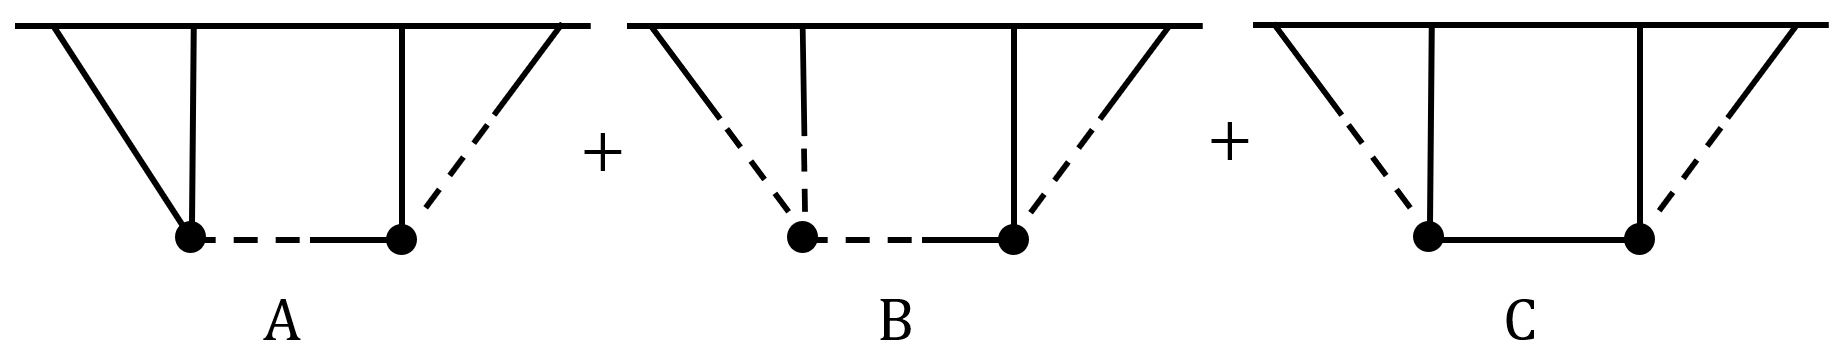
\includegraphics[width=0.9\textwidth]{figures/exchange.png}
\caption{\Eqs{eq:A}、\eqref{eq:B}、\eqref{eq:C} で計算する三つの図。}
\label{fig:exchange}
\end{figure}

\Fig{fig:exchange} の第一の図は次式で与えられる。

\begin{align}\label{eq:A}
A =& 2\left(i \frac{\lambda}{2}\right)^2(-i)\int_{-\infty(1\pm i \epsilon)}^{t_0} \dd t_1 \int_{-\infty(1\pm i \epsilon)}^{t_0} \dd t_2  \\
&\left[ G^K(k_1; t_0,t_1)   G^K(k_2; t_0,t_1)G^R(k_S; t_2,t_1)   G^K(k_3; t_0,t_2)  G^R(k_4; t_0,t_2)+ \mathrm{perms}.\right] \nonumber
\end{align}

Keldysh 伝播関数が純虚数なので、これは明らかに実数である。置換は交換の両側の $E_1\leftrightarrow E_2$、$E_3\leftrightarrow E_4$ と、交換の二つの部分極 $(E_1,E_2)\leftrightarrow(E_3,E_4)$ にわたる。先頭の対称性因子 $2$ は、A 図の左頂点の二本の脚から交換に入る脚を選べることによる。$A\equiv A_1+A_2$ とすると、

\begin{align}
    A_1 =&  \frac{\lambda^2}{16 E_1 E_2 E_3 E_4} \frac{1}{E_T E_L E_R} \left[1- \frac{E_T(E_T-E_s)}{(E_{L} - 2E_s)(E_{R} - 2E_s)}  \right] 
\end{align}

および

\begin{align}
A_2 =&-  \frac{\lambda^2 }{16 E_1 E_2 E_3 E_4} \Bigg\{ \frac{E_{34}}{(E_{134}-E_2)(E_{234}-E_1)\left[(E_1-E_2)^2 - E_s^2\right]} \nonumber \\
&\qquad \qquad + \frac{E_{12}}{(E_{123}-E_4)(E_{124}-E_3)\left[(E_3-E_4)^2 - E_s^2\right]}\Bigg\}
\end{align}

となる。\Fig{fig:exchange} の第二の図は

\begin{align}\label{eq:B}
B =& 6\left(i \frac{\lambda}{2}\right) \left(i \frac{\lambda}{24}\right) (-i) \int_{-\infty(1\pm i \epsilon)}^{t_0} \dd t_1 \int_{-\infty(1\pm i \epsilon)}^{t_0} \dd t_2  \\
&\left[G^R(k_1; t_0,t_1)  G^R(k_2; t_0,t_1)G^R(k_S; t_2,t_1)  G^K(k_3; t_0,t_2)  G^R(k_4; t_0,t_2)+ \mathrm{perms}.\right] \nonumber
\end{align}

である。先頭の対称性因子 $6$ は、B 図で左頂点の二本、右頂点の三本から交換に入る脚を選ぶ自由度による。置換を行うと $B=A_1-A_2$ となり、$A_2$ の寄与が相殺される。最後に \Fig{fig:exchange} の第三の図は

\begin{align}\label{eq:C}
C =& 2\left(i \frac{\lambda}{2}\right)^2 (-i)\int_{-\infty(1\pm i \epsilon)}^{t_0} \dd t_1 \int_{-\infty(1\pm i \epsilon)}^{t_0} \dd t_2  \\
&\left[G^R(k_1; t_0,t_1)  G^K(k_2; t_0,t_1)  G^K(k_S; t_2,t_1)   G^K(k_3; t_0,t_2)  G^R(k_4; t_0,t_2)+ \mathrm{perms}.\right] \nonumber
\end{align}

である。先頭の対称性因子 $2$ は、左頂点の二本の脚から一本を選ぶ自由度による。置換を行うと、

\begin{align}
C=& \frac{ 2 \lambda^2}{16 E_1 E_2 E_3 E_4} \frac{1}{E_L E_R E_s} \frac{(E_L-E_s)(E_R-E_s)}{(E_L-2E_s)(E_R-2E_s)}.
\end{align}

となる。三つの寄与を加えると期待される結果を回復する。

\begin{align}
A+B+C = \frac{2 \lambda^2}{16 E_1 E_2 E_3 E_4} \frac{(E_T+E_s)}{E_T E_L E_R E_s}.
\end{align}

\sectionlink{微分を含むノイズの Langevin 方程式}\label{app:Langevin}

この付録では、Hubbard--Stratonovich 変換 \eqref{eq:HStrick} を修正し、微分を含むノイズ $\pia^{\prime2}$ と $(\partial_i\pia)^2$ を Langevin 方程式に組み込む。同じパワースペクトルを与える二つの方法を示す。

\subsection*{単一のノイズ}

微分を含むノイズを扱うには、結合 $\pia\Os$ に微分演算子 $\mathfrak{D}$ を導入し、

\begin{equation}
\exp\left(i\int d^{4}x a^{4}\mathcal{L}_{2}^{(2)}\right)=\mathcal{N}\int\mathcal{D}[\Os]\;\exp\left[\int d^{4}x a^{4}\left(-\frac{\Os^{2}}{2\beta_{1}}+i\Os\overset{\rightarrow}{\mathfrak{D}}\pia\right)\right],
\end{equation}

とする。ここで

\begin{equation}\label{eq:frakDprop}
(\overset{\rightarrow}{\mathfrak{D}}\pia)^{2}=\pia^{2}+\frac{\beta_{4}-\beta_{2}}{\beta_{1}}\frac{\pia^{\prime2}}{a^{2}}+\frac{\beta_{2}}{\beta_{1}}\frac{(\partial_{i}\pia)^{2}}{a^{2}}.
\end{equation}

である。このように Gaussian ノイズ $\Os$ に作用する微分演算子を通じて、微分を含むノイズを Langevin 方程式に組み込める。

\begin{equation}
\widehat{D}_{R} [\pi(\eta)] =\frac{\left[a^{4}(\eta)\Os(\eta)\right]\overset{\leftarrow}{\mathfrak{D}}}{a^{2}(\eta)}.
\end{equation}

右辺がゼロでない微分方程式の解は、$\widehat{D}_R$ の Green 関数を用いて次のように表される。

\begin{equation}
\pi_{\bfk}(\eta)=\int_{-\infty}^{0}d\eta'\; G^{R}(k;\eta,\eta')\left[a^{4}(\eta')\delta\mathcal{O}_{S}(\bfk, \eta')\right]\overset{\leftarrow}{\mathfrak{D}},
\end{equation}

部分積分によりノイズに微分が作用しない形にできる。\footnote{境界項は、無限の過去では Bunch--Davies 真空により、$\eta^\prime=\eta$ の等時刻極限では遅延境界条件により消える。}

\begin{equation}
\pi_{\bfk}(\eta)=-\int_{-\infty}^{0}d\eta'\; a^{4}(\eta')\delta\mathcal{O}_{S}(\bfk,\eta')\overset{\rightarrow}{\mathfrak{D}}\left[G^{R}(k;\eta,\eta')\right].
\end{equation}

通常の方法でパワースペクトルを計算すると、

\begin{equation}
\langle\pi_{\bfk}(\eta)\pi_{\bfk'}(\eta)\rangle=2\beta_{1}(2\pi)^3{\delta}(\bfk+\bfk')\int_{-\infty}^{0} d\eta'\;a^{4}(\eta')\overset{\rightarrow}{\mathfrak{D}}\left[G^{R}(k;\eta,\eta')\right]\overset{\rightarrow}{\mathfrak{D}}\left[G^{R}(k;\eta,\eta')\right].
\end{equation}

となる。性質 \eqref{eq:frakDprop} を用いて被積分関数を簡単にすると、

\begin{align}
2\beta_{1}\overset{\rightarrow}{\mathfrak{D}}\left[G^{R}(k;\eta,\eta')\right]&\overset{\rightarrow}{\mathfrak{D}}\left[G^{R}(k;\eta,\eta')\right]= 2\beta_{1}\left[G^{R}(k;\eta,\eta')\right]^{2} \Bigg.\\
+&2(\beta_{4}-\beta_{2})\frac{\left[\partial_{\eta'}G^{R}(k;\eta,\eta')\right]^{2}}{a^{2}(\eta)}+2\beta_{2}\frac{\left[\partial_{i}G^{R}(k;\eta,\eta')\right]^{2}}{a^{2}(\eta)}.\nonumber
\end{align}

を得る。この形から、\Sec{sec:Pk} で導いたパワースペクトル \eqref{eq:Keldyshreff} と一致することが明らかである。

\subsection*{三つのノイズ}

微分を含むノイズを組み込む別の方法は、Hubbard--Stratonovich 変換 \eqref{eq:HStrick} で $\pia$ に微分結合する新しい Gaussian 場 $\Os^{(i)}$ を導入することである。時間微分のノイズについては、変換は次の形になる。

\begin{align}
\exp\Bigg[-&\int d^{4}x a^{2}(\beta_{4}-\beta_{2})\pia^{\prime2}\Bigg]=\mathcal{N}^{(2)}\int\mathcal{D}[\Os^{(2)}]\\
&\times\;\exp\left\{\int d^{4}x a^{4}\left[-\frac{[\Os^{(2)}]^{2}}{4\beta_{1}}+i\sqrt{\frac{\beta_{4}-\beta_{2}}{\beta_{1}}}\frac{\pia'}{a}\Os^{(2)}\right]\right\}.\nonumber
\end{align}

空間微分のノイズについては、Laplacian の平方根を考える必要がある。

\begin{align}
\exp\Bigg[-&\int d^{4}x a^{2}\beta_{2}(\partial_{i}\pia)^{2}\Bigg]=\mathcal{N}^{(3)}\int\mathcal{D}[\Os^{(3)}]\\
&\times\;\exp\left\{\int d^{4}x a^{4}\left[-\frac{[\Os^{(3)}]^{2}}{4\beta_{1}}+i\sqrt{\frac{\beta_{2}}{\beta_{1}}}\frac{1}{a}\Os^{(3)}\sqrt{\nabla^{2}}\pia\right]\right\}.\nonumber
\end{align}

Langevin 方程式は次のように修正される。

\begin{equation}
\widehat{D}_{R}[\pi_{\bfk}(\eta)]=a^{2}(\eta)\Os^{(1)}-\frac{1}{a^{2}(\eta)}\partial_{\eta}\left[\sqrt{\frac{\beta_{4}-\beta_{2}}{\beta_{1}}}a^{3}(\eta)\Os^{(2)}\right]-ka(\eta)\sqrt{\frac{\beta_{2}}{\beta_{1}}}\Os^{(3)}.
\end{equation}

ノイズの統計は、各ノイズを添字で区別する行列構造を持つ。

\begin{equation}
\langle\delta\mathcal{O}^{(a)}_{S}(\bfk, \eta_{1})\delta\mathcal{O}^{(b)}_{S}(\bfk', \eta_{2})\rangle=2\beta_{1}H^{4}\eta_{1}^{4}(2\pi)^{3}\delta(\bfk+\bfk')\delta(\eta_{1}-\eta_{2})\delta^{ab}.
\end{equation}

この方法により、\Sec{sec:Pk} の経路積分で得た Keldysh 伝播関数 \eqref{eq:Keldyshreff} を、Langevin 方程式から完全に回復する。
\end{document}
